% Drucklegung
% ===========

\documentclass[11pt, a4paper, twoside, numbers = noenddot, headings = optiontoheadandtoc, captions = nooneline]{scrbook}	% BCOR = Bindungskorrektur; noenddot entfertn Pkt nach Kap.-Nr., nooneline: alle Bildunterschiften sind immer linksbündlig
\usepackage[ngerman]{babel}

% Schriften
% ---------
\usepackage{ebgaramond}		% Schriftart auf Garamond
\usepackage[semibold, light]{sourcesanspro}
\usepackage[T1]{fontenc}
\usepackage{tipa}	% Nutzung phonetischer Zeichen
\setkomafont{disposition}{\normalfont\bfseries}

% Seitenstil
% ----------
\usepackage[top = 30mm, bottom = 20mm, inner = 30mm, outer = 20mm]{geometry}
%\setlength\topmargin{-5.6mm}
%\setlength\headheight{6mm}
%\setlength\headsep{5mm}
\setlength{\columnsep}{6mm}	% Plastz zwischen den Spalten
\usepackage{fancyhdr}
\pagestyle{fancy}

% https://tex.stackexchange.com/questions/228362/get-sectionmark-in-fancyhdr-without-chapter-number/228363#228363
\renewcommand{\chaptermark}[1]{\markboth{#1}{}}	% entfernt die Nummerierung der Kapitel aus der Kopfzeile
\renewcommand{\sectionmark}[1]{\markright{#1}}	% entfernt die Nummerierung der Unterkapitel aus der Kopfzeile

\fancyhead{}
\fancyfoot{}
\fancyhead[LE]{{\fontsize{7.7pt}{10pt}\textsf{\thepage}}}
\fancyhead[RE]{{\fontsize{7.7pt}{10pt}\textsf{\MakeUppercase{\leftmark}}}}
\fancyhead[RO]{{\fontsize{7.7pt}{10pt}\textsf{\thepage}}}
\fancyhead[LO]{{\fontsize{7.7pt}{10pt}\textsf{\MakeUppercase{\rightmark}}}}
\renewcommand{\headrulewidth}{0.5pt}
% Seiteneinstellung für plain -> Seiten mit Kapitelanfang
\fancypagestyle{plain}{%
	\fancyhead{}
	\fancyfoot{}
	\renewcommand{\headrulewidth}{0pt}
}

% Fließtext
% ---------
\usepackage{setspace}


% Überschriften
% -------------
\addtokomafont{chapter}{\fontsize{17}{24}\sffamily\mdseries}
%\addtokomafont{section}{\MakeUppercase}
\addtokomafont{section}{\fontsize{13}{17}\sffamily\mdseries}
\addtokomafont{subsection}{\fontsize{11}{16}\sffamily\mdseries}
\addtokomafont{subsubsection}{\fontsize{11}{16}\sffamily\mdseries}
\addtokomafont{paragraph}{\fontsize{10}{14}\sffamily}

% Fußnoten
% --------
%\usepackage{footmisc}
\let\raggedfootnote\raggedright % linksbündige Fußnoten
\addtokomafont{footnote}{\fontsize{8.2pt}{12pt}\selectfont} % größe der Fußnoten
\addtokomafont{footnotelabel}{\sffamily\mdseries}
\addtokomafont{footnotetext}{\sffamily\mdseries}
\deffootnote{8mm}{1em}{
	\makebox[8mm][l]{\thefootnotemark}}	% Einzug der Fußnoten
\setfootnoterule[0.5pt]{25mm}
\usepackage{chngcntr}
\counterwithout{footnote}{chapter}	% Fußnotennummerierung läuft über die Kapitel hinweg
\interfootnotelinepenalty=0	% =0 ermöglicht einfaches Umbrechen vs. =1000 verhindert den Umbruch von Fußnoten 


% Abbildungen & Tabellen
% ----------------------
\usepackage{caption}
\usepackage{graphicx}
\usepackage{morefloats}	% mehr float-Obj können verarbeitet werden
\usepackage[labelfont = bf]{caption}	% fette Abbildungsnummern
\usepackage{subcaption}

\DeclareCaptionFont{captionfont}{\fontsize{7.5}{10}\sffamily}	% Größe von Abb./Tab. Beschriftungen

% format = hang für hängenden Einzug
\captionsetup[figure]{font = captionfont, labelfont = bf, labelsep = quad, justification=raggedright, format = plain}	% Abstand zwischen Nr und Text

\captionsetup[subfigure]{labelfont = bf, labelsep = quad, labelformat = mysublabelfmt, font = captionfont, justification=raggedright, format = plain}	% keine Klammern um die Bezeichnung der Subfigure
\renewcommand{\thesubfigure}{\Alph{subfigure}}	% große Buchstaben als Bezeichner

\captionsetup[table]{font = captionfont, labelfont = bf, labelsep = quad, justification=raggedright, format = plain}	% Abstand zwischen Nr und Text

\captionsetup[subtable]{labelfont=bf, labelsep = quad, labelformat = mysublabelfmt, font = captionfont, justification=raggedright, format = plain}	% keine Klammern um die Bezeichnung der Subfigure
\renewcommand{\thesubtable}{\Alph{subtable}}	% große Buchstaben als Bezeichner

\addto\captionsngerman{%
	\renewcommand{\figurename}{Abbildung}
	\renewcommand{\tablename}{Tabelle}
}

\newenvironment{sftabular}[1]%
{\sffamily \begin{tabular}{#1}}%
	{\end{tabular}}

% Tafeln
% ------
% neue Umgebung definieren (http://tex.stackexchange.com/questions/6478/new-figure-environment)
\usepackage{float}

%\newcommand\fs@plates{}
\floatstyle{plain}
\newfloat{pl}{thp}{lop}
\floatname{pl}{Tafel}
\captionsetup[pl]{font = captionfont, labelfont = bf, labelsep = quad}	% Abstand zwischen Nr und Text

% Literatur
% ---------
\usepackage[style = authoryear-icomp, 
 sorting = nyt, 
 backend = biber, 
 uniquename = false,
 uniquelist = false,
 language = auto, 
 mincitenames = 1,
 maxcitenames = 2, % nach 2 Autoren bereits u.a.
 maxbibnames = 100, 
 giveninits = true, % kürzt die Vornamen ab
 dashed = true, 
 ibidtracker = true,
 mergedate = false]{biblatex}
\bibliography{bib/bib.bib}
%\addbibresource{Lit.bib}
\renewcommand*{\mkbibnamefamily}[1]{\textsc{#1}}	% Autorennamen in Kapitälchen
%\renewcommand*{\mkbibnamelast}[1]{\textsc{#1}}	% bei älterem biblatex (<=3.3)
\renewcommand*{\bibfont}{\footnotesize}	% kleiner Text im Literaturverzeichnis

\renewcommand*{\postnotedelim}{\addcolon\space}	% Doppelpunkt anstatt Komma vor Seitenzahl
%\renewcommand*{\postnotedelim}{\ifciteibid{\addcolon\space}{\space}}

\renewcommand*{\finalnamedelim}{\addspace\&\space} % &-Zeichen zwischen Autoren

\DeclareFieldFormat{pages}{#1}	% entfernt 'S.' in Kurzzitaten & Literaturliste
\DefineBibliographyStrings{german}{%
	page = {{}{}},
	pages = {{}{}},
	% andothers = {{et\,al\adddot}},
}

% Bibliography

\AtEveryBibitem{
 \clearlist{publisher}
 %\clearfield{month}
 \clearfield{issn}
 \clearfield{isbn}
 \clearfield{url}
 \clearfield{doi}
}  

\renewcommand{\labelnamepunct}{\quad}         % Geviertleerzeichen zwischen Autor (2006) und Titel im LV
%\renewcommand{\bibnamedash}{--\hspace{7mm}}      % (Halbgeviert) als Ersatz für wiederkehrende Autoren oder Herausgeber in der Bibliografie verwendet wird
\renewcommand{\bibpagespunct}{\addcolon\addspace} % Seitenzahlen abtrennen mit : 
\DeclareFieldFormat{title}{\normalfont{#1}}    % Titel in normaler Schrift im LV
\DeclareFieldFormat[article,incollection]{title}{#1}      % Titel in Journals und Sammelbänden nicht in "Hochkomma" im LV
%\DeclareFieldFormat{myjournaltitle}{#1} % Zeitschriftentitel kursiv (funktioniert nur ohne \emph{} Auszeichnung!???)
\DeclareFieldFormat{series}{\emph{#1}} % Reihentitel kursiv
\DeclareFieldFormat{issuetitle}{#1} % Ausgabetitel nicht kursiv
\DeclareFieldFormat{maintitle}{#1} % Sammelbandtitel nicht kursiv
\DeclareFieldFormat{booktitle}{#1} % Sammelbandtitel nicht kursiv


\setlength\bibitemsep{1.8mm}   % Abstand zwischen Einträgen im Literaturvereichnis (1.8mm) im LV
\setlength\bibhang{9mm}
\renewcommand{\bibnamedash}{--\hspace{7mm}}

% Kein In: bei Artikeln 
\renewbibmacro{in:}{   
\ifentrytype{article}{}{\printtext{\bibstring{in}\intitlepunct}}}

% Volume gefolgt von Nummer in Klammern  
\DeclareFieldFormat[article]{number}{\mkbibparens{#1}}
\renewbibmacro*{volume+number+eid}{%
	\printfield{volume}%
	\printfield{number}}     

%% Bei Artikeln die zweite Jahreszahl nicht in Klammer setzen
\renewbibmacro*{issue+date}{%
	\setunit{\addcomma\space}% NEW
	%  \printtext[parens]{% DELETED
	\iffieldundef{issue}
	{\usebibmacro{date}}
	{\printfield{issue}%
		\setunit*{\addspace}%
		%       \usebibmacro{date}}}% DELETED
		\usebibmacro{date}}% NEW
	\newunit}

%%%  Inbook, Incollection, Inproceedings
%  Editor nach dem In: und vor dem Titel
\renewbibmacro*{in:}{
	\ifentrytype{incollection}{%
		\DeclareNameAlias{editor}{first-last}
		\printtext{In: }
		\ifnameundef{editor}
		{}
		{\printnames{editor}%
			\addspace 
			\usebibmacro{editorstrg} % \mkbibparens{\usebibmacro{editorstrg}}, in diesem Falle keine Klammern nach Autor, ed. (2016)
			%\mkbibparens{\usebibmacro{editorstrg}}
			\setunit{\addcomma\addspace}% 
		}%
		\usebibmacro{maintitle+booktitle}
		\clearfield{maintitle}    %% Folgende Eintr�ge sollen nun nicht noch einmal ausgegeben werden 
		\clearfield{booktitle}
		\clearfield{volume}
		\clearfield{part}
		\clearname{editor}
	}
	{}%
}

%  ed./eds. immer in Klammern (auch nach Erstautor!)
\DeclareFieldFormat{editortype}{\mkbibparens{#1}}

% kein Komma vor ed. (z.B. wenn in 1. Zeile nach Erstautor)
\usepackage{xpatch}
\xpatchbibmacro{bbx:editor}
{\addcomma\space}{\addspace}{}{}    

%%%%%  Inbook, Incollection, Inproceedings, book
%% Ort und Jahr in Klammern, ohne Komma (Köln 2017)
\renewbibmacro*{publisher+location+date}{%
	%\printtext[parens]{%
	{%
		%\printlist{publisher}%   % Verlag wird nicht ausgegeben
		%\iflistundef{location}
		%{\setunit*{\addcomma\space}}
		%{\setunit*{\addcolon\space}}%
		\printlist{location}%
		\setunit*{\space}%
		\usebibmacro{date}%
	}\newunit%
}

%% Kein Punkt nach Titel bei book
%\xpatchbibdriver{book}
%{\newunit\newblock\usebibmacro{publisher+location+date}}{%
%	\setunit{\addspace}\newblock%
%	\usebibmacro{publisher+location+date}%
%}{}{}      
%
%% Kein Punkt nach Titel bei incollection 
%\xpatchbibdriver{incollection}
%{\newunit\newblock\usebibmacro{publisher+location+date}}{%
%	\setunit{\addspace}\newblock%
%	\usebibmacro{publisher+location+date}%
%}{}{}      
%
%% Kein Punkt nach Titel bei inbook 
%\xpatchbibdriver{inbook}
%{\newunit\newblock\usebibmacro{publisher+location+date}}{%
%	\setunit{\addspace}\newblock%
%	\usebibmacro{publisher+location+date}%
%}{}{}  




%\setstretch{1.3333} % 10pt has 12pt baselineskip
%\setlength\parskip{\z@ \@plus 1\p@}
\setlength\parindent{6mm}
\setlength\partopsep{6mm}

\usepackage{t1enc}
\usepackage[utf8]{inputenc}

\usepackage{amsmath}
\usepackage{amssymb}

\usepackage{enumitem}
\setitemize{leftmargin=*} % entfernt die Einrückung der item-Umgebung
\setenumerate{leftmargin=*} % entfernt die Einrückung der item-Umgebung

\usepackage[autostyle = true, german = guillemets]{csquotes}	% ermöglicht die Nutzung von franz. Anführungszeichen - mit \enquote{} beziehungsweise \enquote*{}

\usepackage{todonotes}				% lässt todo's im code zu
\usepackage[hidelinks]{hyperref}	% erstellt die farbigen Links im PDF und gibt die Möglichkeit URLs einzugeben

\urlstyle{same}


% #########################################################
% # ALTER HEAD                                            #
% #########################################################




\usepackage{mdwlist} % Listen ohne Zwischenabstand




% Abbildungen & Tabellen
% ======================

\makeatletter	% erzeugt in dem \ref auf subfigures eine Ausgabe : Fig.Subfig -- bspw. (Abb. 32.A)
\renewcommand\p@subfigure{\thefigure}
\renewcommand\thesubfigure{.\Alph{subfigure}}
\DeclareCaptionLabelFormat{mysublabelfmt}{\Alph{sub\@captype}}
\makeatother

\makeatletter	% erzeugt in dem \ref auf subfigures eine Ausgabe : Fig.Subfig -- bspw. (Abb. 32.A)
\renewcommand\p@subtable{\thetable}
\renewcommand\thesubtable{.\Alph{subtable}}
\DeclareCaptionLabelFormat{mysublabelfmt}{\Alph{sub\@captype}}
\makeatother

\usepackage{array}	% liefert vertikale Ausrichtung der Zelleninhalte von Tabellen mit m{}
\newcolumntype{P}[1]{>{\raggedright\arraybackslash}p{#1}}	% linksbündige Tabellen mit P
\newcolumntype{R}[1]{>{\raggedleft\let\newline\\\arraybackslash\hspace{0pt}}m{#1}}	% rechtsbündige Tabellen mit R

\usepackage{adjustbox}	% ermöglichst das Beschneiden von Grafiken

\usepackage{longtable}
\usepackage{supertabular}
\usepackage{arydshln}	% gestrichelte Linien mit \hdashline & \cdashline
\usepackage{multirow}	% http://ctan.org/pkg/multirow
\usepackage{multicol}
\usepackage{makecell}
\usepackage{booktabs}	% lässt \top-, \mid- & \bottomrule in Tab zu

\usepackage{chngcntr}	% setzt kontinuierliche Abbildungs- & Tabellennummerierung
\counterwithout{figure}{chapter}
\counterwithout{table}{chapter}







\renewcommand*{\figureformat}{\figurename~\thefigure}	% unterdrückt mögliche Sonderzeichen (Pkt.) hinter Abb.-Nr.
\renewcommand*{\tableformat}{\tablename~\thetable}		% vertikale Zellen in Tabelle

%\newcommand*\rot{\rotatebox{90}}						

\graphicspath{ {images/} }	% Bilderordner

\usepackage[figuresright]{rotating}	% Provides {sideways}{sidewaysfigure}{sidewaystable} environments; siehe https://en.wikibooks.org/wiki/LaTeX/Rotations
\usepackage{afterpage}	% longtable to the top of the next page

\usepackage{tikz}
\usetikzlibrary{shapes,arrows}
\usetikzlibrary{calc,
	arrows,decorations.pathmorphing,
	backgrounds,fit,positioning,shapes.symbols,chains}
\usetikzlibrary{decorations.pathreplacing}
\usepackage{smartdiagram}

% für Abbildungen die in Spaltenbreite gesetzt werden sollen
\newenvironment{Figure}
{\par\medskip\noindent\minipage{\linewidth}}
{\endminipage\par\medskip}

% Listen
% ======
% neue Umgebung definieren (http://tex.stackexchange.com/questions/6478/new-figure-environment)
\usepackage{float}
\floatstyle{plain}
\newfloat{ls}{thp}{lop}
\floatname{ls}{Liste}
\captionsetup[ls]{labelsep = quad}	% Abstand zwischen Nr und Text




% \input{header.tex}

% Text mit Kreis umschließen
% ==========================
\usetikzlibrary{arrows}
\usetikzlibrary{shapes}
\newcommand*\circled[1]{\tikz[baseline=(char.base)]{
            \node[shape = circle, draw, inner sep = 2pt] (char) {#1};}}

% =================================================================

%\usepackage{showframe}
\usepackage{blindtext}

\includeonly{chpt/1_Einleitung}	% ermöglichst, nur einzelne Kapitel auszugeben

%\sloppy	% großzügigeere Formatierung mit weniger Trennungen

\begin{document}

\urlstyle{same}	% URLs in der gleichen Schriftart wie der Text
\pagenumbering{gobble}
\title{Archäologische Untersuchungen\\zur eisenzeitlichen Besiedlungsgeschichte des nordwestlichen Kongobeckens}
\author{\parbox{.7\textwidth}{\normalsize\centering
 {Dissertation\\
 zur Erlangung des akademischen Grades\\
 Doktor der Philosophie\\
 in der Philosophischen Fakultät\\
 \vskip 5mm
 der Eberhard Karls Universität Tübingen
 {\LARGE 
 \vskip 25mm
%\textbf{Teil I}
% \textbf{Teil II}
 \vskip 5mm
%\textbf{Text}
}}}}
% \textbf{Anhang}}}}}
% \vskip 5mm
\date{}%
\publishers{\normalsize{%
 vorgelegt von\\
 {\Large Dirk Seidensticker\\[.5ex]}%
 aus Hoyerswerda\\[\baselineskip]
 \the\year				% gibt nur die Jahreszahl aus
 %Stand: \today		% für das genaue Datum
 }}
\lowertitleback{%
 {%
 \begin{tabular}{ll} 
 Hauptberichterstatter: & Prof. Dr. Thomas Knopf\\ 
 Mitberichterstatter: & Prof. Dr. Manfred K. H. Eggert\\ 
 \end{tabular}
 \vskip 5mm
 }%Tag der mündlichen Prüfung: 20.12.2006}%
}

\maketitle
\cleardoublepage

%\clearpage
%\null\vfill
%\thispagestyle{empty}
%\begin{center}
%\textit{Für Katharina}
%\end{center}
%\vfill
%\clearpage

%\cleardoublepage
%
%\pagenumbering{roman}
%\chapter*{Erklärung}
%\begin{multicols}{2}
%\raggedcolumns
%\noindent Ich erkläre hiermit, dass ich die zur Promotion eingereichte Arbeit mit dem Titel: \enquote{Archäologische Untersuchungen zur eisenzeitlichen Besiedlungsgeschichte des nordwestlichen Kongobeckens} selbständig verfasst, nur die angegebenen Quellen und Hilfsmittel benutzt und wörtlich oder inhaltlich übernommene Stellen als solche gekennzeichnet habe. Ich versichere an Eides statt, dass diese Angaben wahr sind und dass ich nichts verschwiegen habe. Mir ist bekannt, dass die falsche Abgabe einer Versicherung an Eides statt mit Freiheitsstrafe bis zu drei Jahren oder mit Geldstrafe bestraft wird.
%\end{multicols}
%\vspace{2.5em}
%\noindent Tübingen, den 04. Oktober 2017
%
%\vspace{0.5em}
%\noindent Dirk Seidensticker



\cleardoublepage
%\pagenumbering{roman}
\thispagestyle{empty}
\section*{Vorwort}
%\addcontentsline{toc}{section}{Vorwort}
%\chapter*{Vorwort}
\addcontentsline{toc}{chapter}{\hspace{1.5em}Vorwort}
\begin{multicols}{2}
\raggedcolumns
\noindent Die vorliegende Untersuchung stellt die überarbeitete Fassung meiner im Oktober 2017 an der Philosophischen Fakultät der Eberhard Karls Universität Tübingen eingereichten Promotionsschrift dar. Nach 2017 erschienene Literatur wurde nur in Einzelfällen eingearbeitet. Ohne die vielfältige Unterstützung zahlreicher Personen und Institutionen wäre diese Arbeit nicht möglich gewesen. Ihnen allen gebührt mein aufrichtiger Dank.

Besonderen Dank schulde ich Manfred K.~H. Eggert, der mir nicht nur das Fundmaterial zur Bearbeitung überließ, sondern mir durch seine intensive Betreuung auch die Fertigstellung der Arbeit ermöglichte. Nicht minder dankbar bin ich Thomas Knopf für seine konstruktive Unterstützung und Betreuung in der Schlussphase. Peter Breunig (Frankfurt a. M.) danke ich für sein Drittgutachten.

Von 2012 bis 2016 wurde die Arbeit durch Hans-Peter Wotzka, Forschungsstelle Afrika am Institut für Ur- und Frühgeschichte der Universität zu Köln, betreut. Für die wissenschaftliche Begleitung in dieser Zeit gebührt ihm mein Dank. Die vorliegende Arbeit versteht sich auch als Ergänzung zu der von ihm im Jahr 1995 veröffentlichten, wegweisenden Untersuchung zum Fundmaterial des \textit{River Reconnaissance Project} im Inneren Kongobecken. Zudem verdanke ich H.-P. Wotzka die Finanzierung von zwei Radiokohlenstoffdatierungen an Knochen eines Grabes in Maluba am Lua sowie die Analyse von Schlacken durch Jane Humphris und Ole Nordland. 

Die in dieser Arbeit vorgelegten Untersuchungen zur Töpfereitechnologie, insbesondere die Analyse von Makrospuren, wäre nicht ohne die konstante Ermutigung und Unterstützung durch Anne Mayor (Genf) und \mbox{Alexandre} \mbox{Livingstone} Smith (Tervuren) möglich gewesen. Bei einer 2015 durchgeführte Reise nach Genf konnte ich erste Erfahrungen mit der entsprechenden Methodik sammeln. In Tervuren gewährte mir \mbox{Alexandre} Livingstone Smith Einblick in das damals in Bearbeitung befindliche Fundmaterial aus dem nordöstlichen Kongobecken. Für Hilfe und Unterstützung bei der Interpretation der Anschliffe danke ich Heiko Riemer (Köln).\columnbreak

Im Zuge des von Manfred K. H. Eggert geleiteten Projekts zur Restaurierung der Eisenfunde des Gräberfeldes in Campo, Südkamerun, wurden in den Restaurierungswerkstätten des Römisch-Germanischen Zentralmuseums Mainz (RGZM) auch Eisenobjekte der Fundplätze Pikunda und Munda restauriert.

Monika Doll und Angelika Wilk gilt mein Dank für die Bestimmung der Tierknochen und Michael Francken für die Unterstützung bei der erneuten Evaluierung des menschlichen Skelettmaterials. Neben Hilfe bei der Redaktion der Arbeit gilt Christina Vossler-Wolf (alle Tübingen) auch mein Dank für eine Expertise zu potenziell neuzeitlichen Importfunden.

Für anregende Diskussionen und Einsatz bei der Korrektur der Arbeit danke ich Claudia Spohn-Drosihn und Julian Spohn sowie Christina Vossler-Wolf und Marion Etzel (alle Tübingen), Friederike Jesse (Köln), Melanie Augstein (Leipzig), Sebastian Kirschner (München) und Nicole Rupp (Frankfurt). Oliver Vogels (Köln) danke ich für eine Vorlage zur automatisierten Erstellung des Literaturverzeichnisses. Für eine Korrektur der englischsprachigen Zusammenfassung gilt mein Dank Christopher A. \mbox{Kiahtipes} (Tampa); Nicolas Nikis (Cambridge) danke ich für die Durchsicht der französischen Zusammenfassung.

Der finanziellen Unterstützung der Tübinger Universitätsstiftung ist es zu verdanken, dass diese Studie in der vorliegenden Form veröffentlicht werden kann. Für die gute Zusammenarbeit bei der Fertigstellung der Druckvorlage möchte ich mich beim Verlag Tübingen University Press, vor allem bei Sandra Binder bedanken.

Schließlich möchte ich mich ganz besonders bei meiner Partnerin Katharina Jungnickel für ihre konstante Unterstützung bedanken. Sie hat mir geholfen, den Blick in der Schlussphase auf das Wesentliche zu lenken.

Eine phonetisch korrekte Wiedergabe afrikanischer Bezeichnungen und Namen erfolgte aus technischen Gründen nicht. Ebenfalls habe ich bewusst auf ein Verzeichnis der Bildunterschriften verzichtet. Alle bibliographischen Informationen wurden in die Bildunterschriften integriert.

\end{multicols}

%\begin{multicols}{2}
%\vspace{2.5em}
%\noindent Gent, den ??. ??? 2020
%\columnbreak
%\vspace{.5em}
%\noindent Dirk Seidensticker
%\end{multicols}

\setcounter{secnumdepth}{3}		% Tiefe des Inhaltsverzeichnisses
\setcounter{tocdepth}{3}
\tableofcontents
\cleardoublepage

\pagenumbering{gobble}


% für einseitiges Dokument mit zwei Bänden 0_Head anpassen und zwei getrennte Main-Datei (Bd1 & Bd2) machen:
% Bd1: Kap. 1--Ende \printbibliography
% Bd2: Katalog--Tafeln

%\twocolumn % AP-Stil
\part{Text}

\pagenumbering{arabic}

\chapter{Einleitung}
\begin{multicols}{2}
\raggedcolumns
\noindent Die vorliegende Arbeit widmet sich der Auswertung von Funden und Befunden, die in den 1980er Jahren im nordwestlichen Teil des Kongobeckens gemacht wurden. Sie verfolgt dabei das Ziel, Charakter und Verlauf der Besiedlung der Region durch keramikproduzierende, sesshaftlebende und nahrungsmittelanbauende Bevölkerungen nachzuzeichnen. Die in dieser Arbeit diskutierten Materialien stammen aus den Prospektions- und Grabungsaktivitäten des unter der Leitung von Manfred K.~H.~Eggert durchgeführten \textit{River Reconnaissance Project}. Der durch das Projekt erstmals archäologisch erschlossene Untersuchungsraum \parencite[siehe][295 Abb.~16.2]{Eggert.1993} kann in zwei Teile untergliedert werden: zum einen das sogenannte \enquote*{Innere Kongobecken}, welches durch die Prospektionen der linksseitigen Zuflüsse des Kongoflusses repräsentiert wird und Gegenstand einer bis in die Anfänge der 1990er Jahre andauernden Auswertungs- und Publikationstätigkeit war \parencites{Eggert.1980b}{Eggert.1981}{Eggert.1983}{Eggert.1984}{Eggert.1984b}{Eggert.1987}{Wotzka.1995}, sowie das Arbeitsgebiet der vorliegenden Arbeit, das \enquote*{nordwestliche Kongobecken}.\footnote{In Methodik (siehe Kap.~\ref{sec:Quellen}) wie der Beschreibung der keramischen Inventare (siehe Kap.~\ref{sec:Keramiksequenz}, \ref{sec:Horizonte}) orientiert sich die vorliegende Arbeit an der Vorlage der archäologisch erschlossenen Keramiksequenz für das Innere Kongobecken durch Hans-Peter \textsc{Wotzka} (1995).} Dieses, die rechtsseitigen Zuflüsse des Kongo umfassende Gebiet und sein archäologisches Potenzial waren bislang lediglich Gegenstand einiger Vorberichte \parencites{Eggert.1987c}{Eggert.1992}{Eggert.1993}. 

Zur Erarbeitung des räumlich-zeitlichen Bezugssystems wurde die aus dem Arbeitsgebiet vorliegende Gefäßkeramik herangezogen. Neben der Tatsache, dass es sich bei der Gefäßkeramik um die umfangreichste Fundkategorie handelt (Tab.~\ref{tab:Funde_Uebersicht}), eignet sie sich für einen strukturellen Vergleich vor allem aufgrund ihrer potenziellen Präsenz im Alltag der zu untersuchenden Gesellschaften.\footnote{Die zentrale Rolle der Gefäßkeramik bei der Beurteilung prähistorischer Sachkultur wurde zuletzt intensiv von \textcite{Saev.2015} beleuchtet. Gegenstand dieser Untersuchung war die Funktion und Nutzung von Gefäßkeramik im südlichen Ostseeraum vom Neolithikum bis zur Zeitenwende. Ebenfalls sei für die Fragestellung nach der Nutzung und Funktion von prähistorischer Gefäßkeramik auf die Diskussion zwischen \textcites{Riemer.1997}{Wotzka.1997}{Veit.1997} sowie den ethnoarchäologisch ausgerichteten Beitrag von \textcite{Knopf.2009} verwiesen.} Der in dieser Arbeit gewählte Fokus auf die Gefäßkeramik des Arbeitsgebietes setzt eine kontinuierliche Nutzung von Keramik von ihrem ersten archäologisch nachgewiesenen Auftreten bis in die Gegenwart (1985/87) voraus. Diese Annahme bildet in der Folge die Voraussetzung für den diachronen Vergleich (Kap.~\ref{sec:BesiedlGesch}). Ausgangspunkt bildeten dabei die Inventare von insgesamt 19 ausgegrabenen oder hinreichend archäologisch untersuchten Befunden (Katalog~A). Sie wurden um Inventare ergänzt, die bei Surveys innerhalb der modernen Dörfer erschlossen wurden (Katalog B). Die Untersuchung der Quellen vollzieht sich auf zwei Ebenen: Auf die Auseinandersetzung mit Indizien zur Keramiktechnologie (Kap.~\ref{sec:Herstellung}) folgt eine detaillierte Beschreibung von vornehmlich auf stilistischem Wege erarbeiteten keramischen Gruppen, im Weiteren \enquote*{Stilgruppen} genannt (Kap.~\ref{sec:Keramiksequenz}). Sie bilden die grundlegende Entität für die Rekonstruktion der Besiedlungsgeschichte des Arbeitsgebietes (Kap.~\ref{sec:BesiedlGesch}).

Rückschlüsse auf den Charakter sowie Verlauf der Besiedlung des Kongobeckens durch keramikproduzierende, sesshaftlebende und nahrungsmittelanbauende Gruppen lassen sich zum gegenwärtigen Zeitpunkt lediglich auf Grundlage einer sehr eingeschränkten Quellenbasis ziehen. Ausschließlich im Rahmen des \textit{River Reconnaissance Project} wurden bisher systematisch Prospektionen sowie Grabungen durchgeführt. Regionale Abfolgen des keramischen Fundmaterials\footnote{Im weiteren Text wird für die Abfolge der keramischen Stile (siehe auch Kap.~\ref{sec:Sequenzen}) der Begriff \enquote{Sequenz} genutzt.} und daraus ableitbare chronologische Gliederungen liegen lediglich für ausgewählte Regionen vor \parencites{Wotzka.1995}{MbidaMindzie.19951996}{AssokoNdong.20002001}{Clist.20042005}{Lavachery.2010}. Weite Teile Zentralafrikas\footnote{Unter \enquote*{Zentralafrika} wird im Sinne dieser Arbeit das Staatsgebiet Äquatorialguineas, Gabuns, Kameruns, der Demokratischen Republik Kongo (Kongo-Kinshasa), der Republik Kongo (Kongo-Brazzaville) und der Zentralafrikanischen Republik sowie der nördliche Teil Angolas verstanden \parencite[183]{Eggert.2014}. Verschiedentlich werden auch noch der Süden des Tschads sowie Ruanda und Burundi zu diesem Raum hinzu gezählt \parencite[421]{Maret.2005}.} sind bis heute archäologische \textit{terra incognita}.

\section{Arbeitsgebiet und Fragestellung}\label{sec:Arbeitsgebiet}

Unter der Bezeichnung \enquote*{nordwestliches Kongobecken} werden in dieser Arbeit die 1985 und 1987 durch das \textit{River Reconnaissance Project} befahrenen Flussabschnitte des \mbox{Sangha}, \mbox{Ngoko}, Likwala-aux-Herbes, \mbox{Ubangi} und Lua sowie ein kurzes verbindendes Stück entlang des Kongo zwischen der \mbox{Ubangi}- und \mbox{Sangha}-Mündung verstanden (Abb.~\ref{fig:ArbeitsgebietKarte}). Das eigentliche Arbeitsgebiet umfasst administrativ vor allem den nordöstlichen Teil der Republik Kongo (Kongo-Brazzaville) sowie unmittelbar angrenzende Regionen Kameruns, der Zentralafrikanischen Republik und der Demokratischen Republik Kongo (Kongo-Kinshasa). Im nördlichen Teil, entlang des oberen \mbox{Ubangi}, deckt das Arbeitsgebiet die Grenzen der heutigen Provinzen Süd-\mbox{Ubangi} sowie Nord-\mbox{Ubangi} ab.

\begin{figure*}[p]
	\centering
	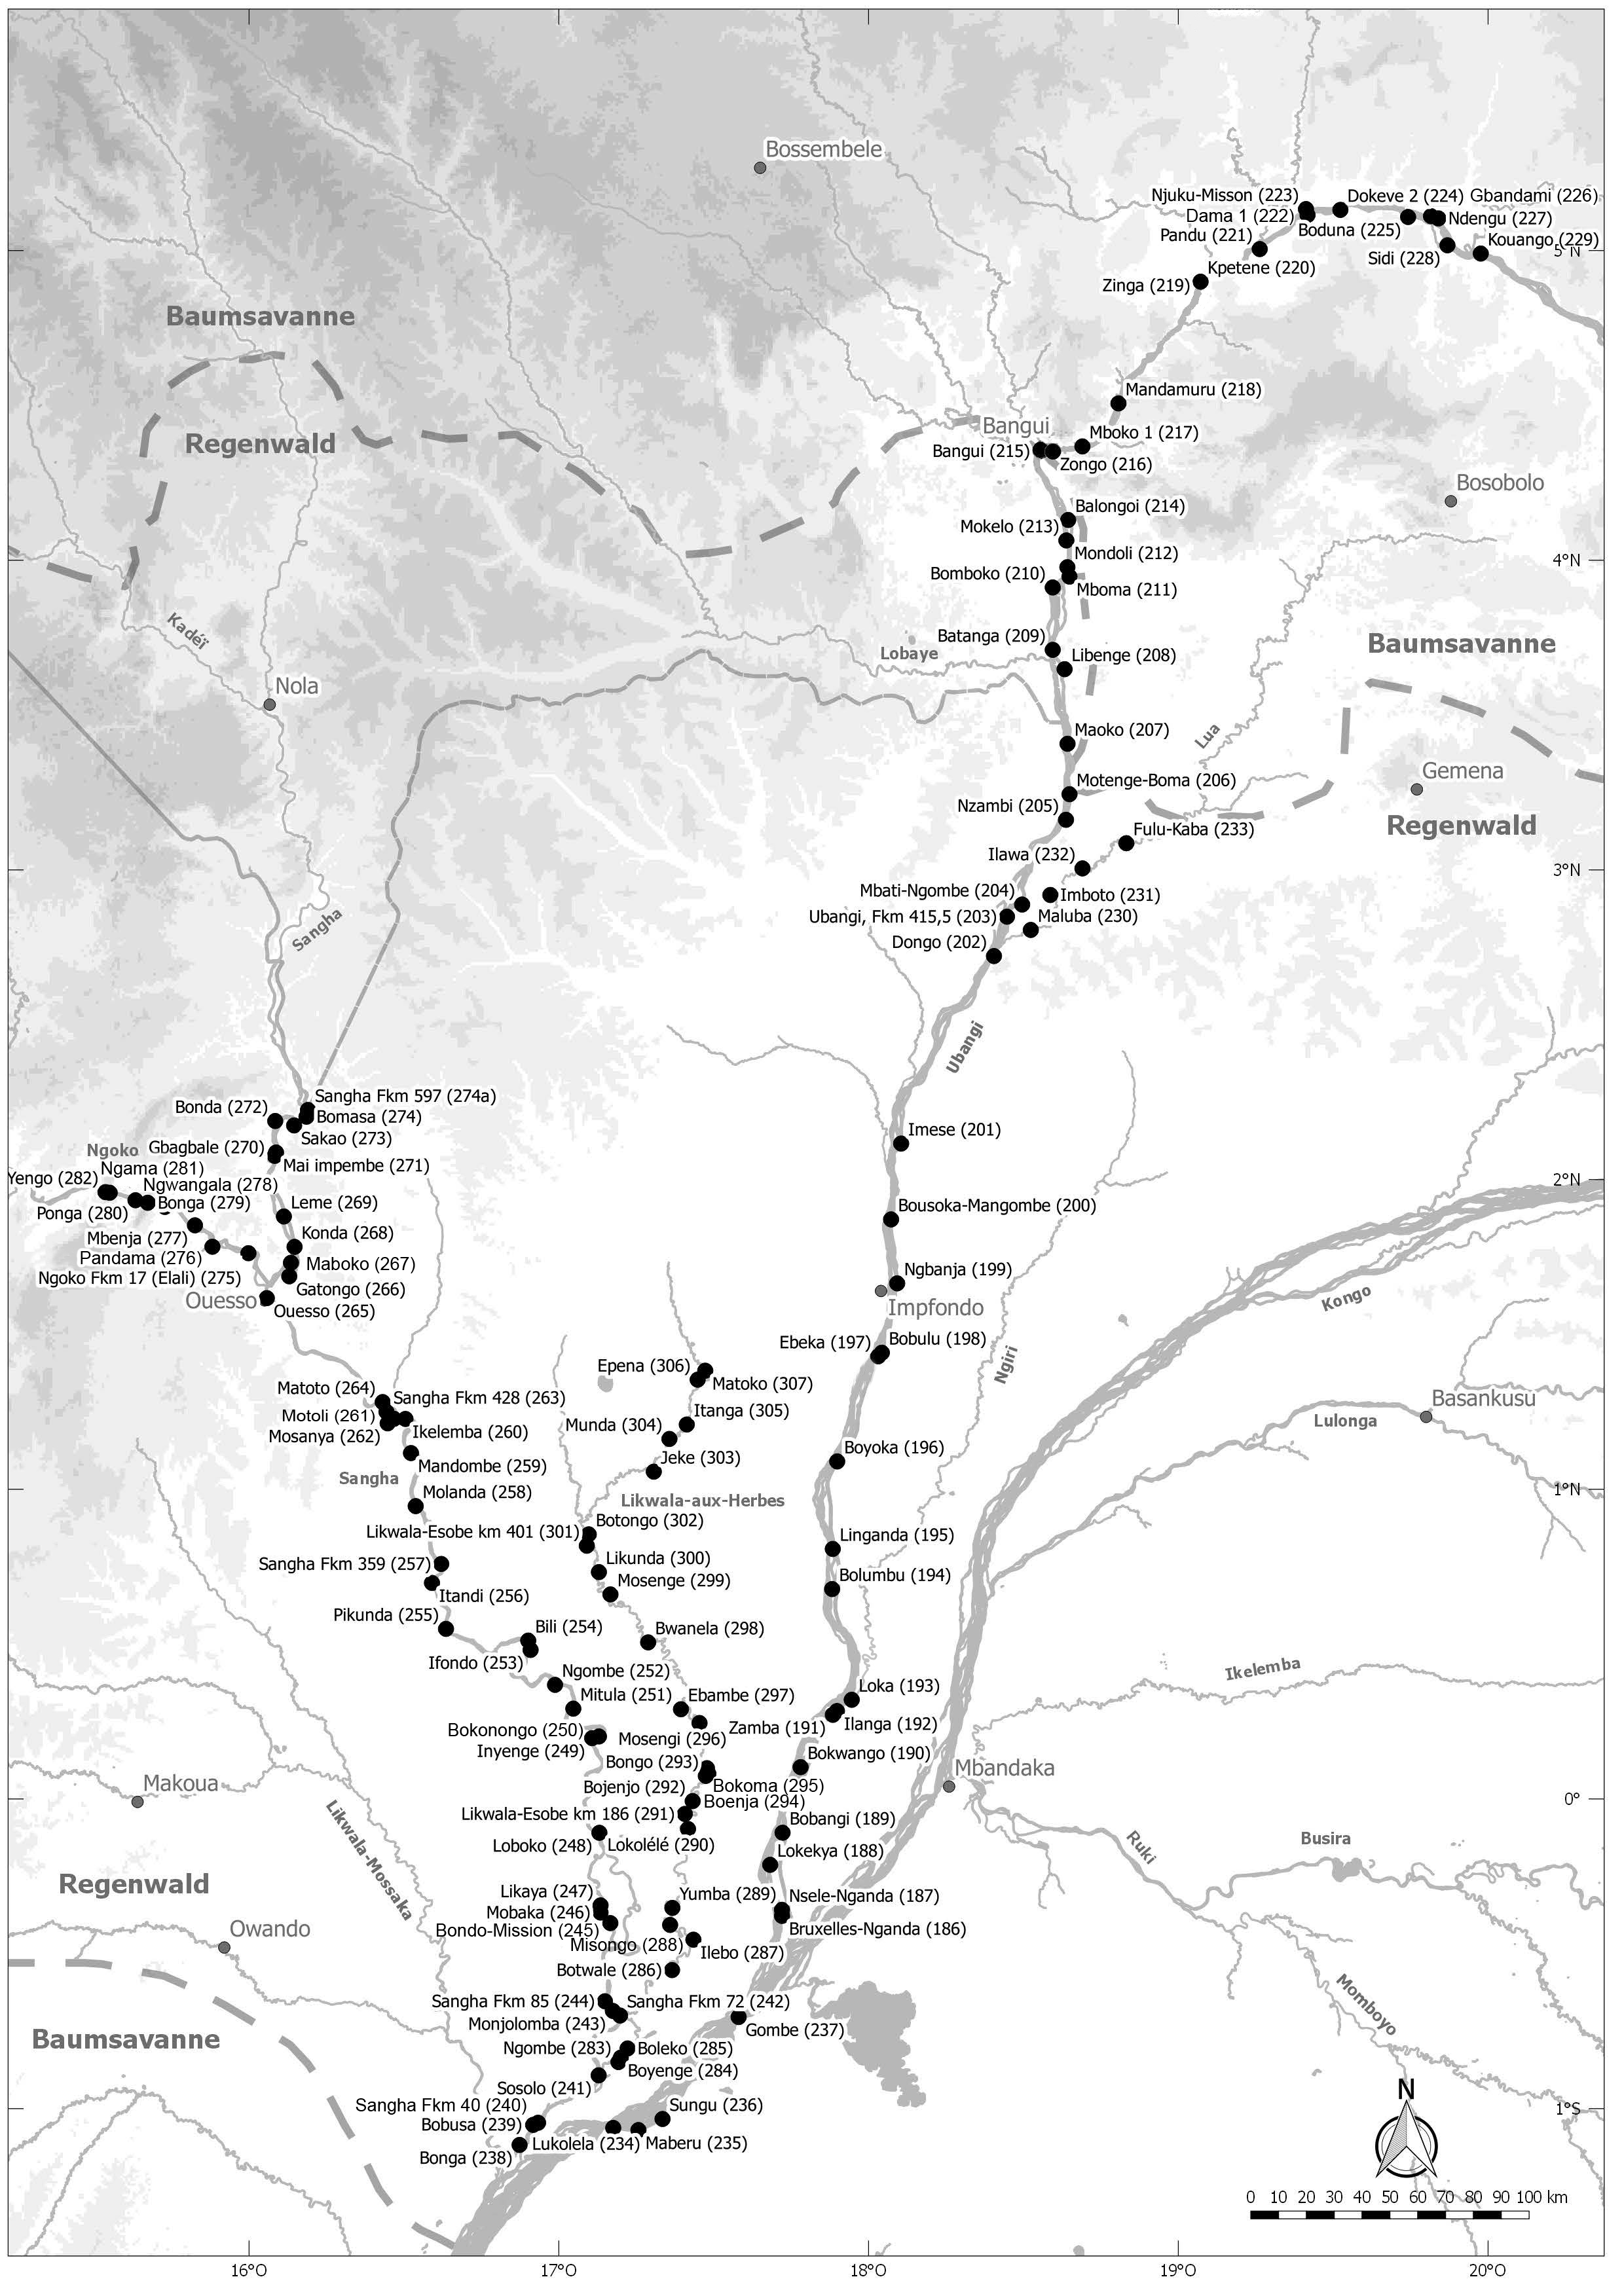
\includegraphics[width=\textwidth]{fig/FundstellenMap.jpg}
	\caption{Arbeitsgebiet: Untersuchte Fundstellen}
	\label{fig:ArbeitsgebietKarte}
\end{figure*}

Das Arbeitsgebiet beschreibt einen Nord--Süd-Transekt von der Feuchtsavanne nördlich von Bangui (Zentralafrikanische Republik) bis in den äquatorialen Regenwald südlich von Mba\-ndaka (Demokratische Republik Kongo). In Nord--Süd-Richtung erstreckt es sich über 700\,km, während es in Ost--West-Richtung annähernd 500\,km groß ist. Alle Fundstellen liegen zwischen 289--390\,m\,ü.\,NN.\footnote{Die Höhen der Fundstellen wurden einem SRTMv3-Datensatz mit einer Grundauflösung von 3 Bogensekunden beziehungsweise etwa 90\,m entnommen (Quelle NASA/USGS; \url{https://earthexplorer.usgs.gov} Zugriff: 04.\,10.\,2014).}

Die Feldarbeiten des \textit{River Reconnaissance Project} in der zweiten Hälfte der Kampagne von 1985 sowie während der Kampagne von 1987 deckten etwa 2130\,km der Flussläufe des \mbox{Ubangi}, Lua, \mbox{Sangha}, \mbox{Ngoko} und \mbox{Likwala}-\mbox{aux}-\mbox{Herbes} ab (Tab.~\ref{tab:ArbeitsgebietFlussstrecken}). Ausgehend von seiner Mündung in den \mbox{Sangha}, die etwa 3\,km nördlich von Ouesso (Fpl.~265) liegt, wurde der \mbox{Ngoko} auf einer Strecke von etwa 80\,km stromauf prospektiert.\footnote{Der untere Abschnitt des Dja, der in Kamerun entspringt, wird ab dem Punkt, an dem er die Grenze zwischen Kamerun und der Republik Kongo bildet (2$^\circ$12$'$25$''$~N, 14$^\circ$35$'$42$''$~O) als \enquote*{\mbox{Ngoko}} bezeichnet. In Yengo (Fpl.~282) musste die Prospektion aufgrund der Malaria-Erkrankung eines Mitarbeiters vorzeitig beendet werden.\label{ftn:DjaNgoko}} Der \mbox{Sangha} bildet den Unterlauf des Kadeï, der in Nordkamerun nahe Garoua-Bouleï entspringt und ab Nola (Zentralafrikanische Republik) als \mbox{Sangha} bezeichnet wird. Der Fluss mündet bei Mossaka, etwa 220\,km südwestlich von Mbandaka in den Kongo. Er wurde auf einer Länge von fast 600\,km bis an das Dreiländereck der Republik Kongo, Kamerun und der Zentralafrikanischen Republik knapp nördlich von Bomasa (Fpl.~274) befahren. Zwischen den Flüssen \mbox{Sangha} und \mbox{Ubangi} liegt der Likwala-aux-Herbes, der auch als \enquote*{Likwala-Esobe} oder \enquote*{Likouala-aux-Herbes} bezeichnet wird und nordwestlich des Lac Tele entspringt. Der \mbox{Likwala}-\mbox{aux}-\mbox{Herbes} wurde insgesamt auf einer Strecke von über 500\,km prospektiert, bis zur nicht passierbaren Brücke bei Matoko (Fpl.~307).\footnote{Der Fluss darf nicht mit dem Likwala-Mossaka verwechselt werden, der auf einigen Karten nur mit der Bezeichnung \enquote*{Likwala} verzeichnet ist. Er verläuft westlich des \mbox{Sangha} und mündet bei Mossaka, wie auch der \mbox{Sangha}, in den Kongo.} Der \mbox{Ubangi} zählt zu den größten Zuflüssen des Kongo und bildet die Grenze zwischen der Demokratischen Republik Kongo und der Zentralafrikanischen Republik sowie der Republik Kongo. Er entspringt aus dem Zusammenfluss von Uele und Mbomou bei Yakoma (Demokratische Republik Kongo) und mündet etwa 90\,km südwestlich von Mbandaka in den Kongo. Der \mbox{Ubangi} wurde auf einer Strecke von etwa 850\,km, bis Kouango (Fpl.~229) befahren. Der Lua ist neben dem Ngiri einer der größten linksseitigen Zuflüsse des \mbox{Ubangi}. Er mündet bei Dongo (Fpl.~202) in den \mbox{Ubangi} und wurde auf einer Strecke von etwa 100\,km bis Fulu-Kaba (Fpl.~233) prospektiert.

\vspace{1.5em}
\noindent Durch diese Feldarbeiten der 1980er Jahre ließen sich für die in dieser Arbeit präsentierte Erstbearbeitung der Befunde und Funde aus dem nordwestlichen Kongobecken eine Reihe von Fragestellungen und Arbeitsziele formulieren:
\begin{itemize*}
\item Die Auswertung der ausgegrabenen Befunde in Maluba (Fpl.~230; Kat.-Nr.~1--5), Bobusa (Fpl.~239; Kat.-Nr.~6--7), Pikunda (Fpl.~255; Kat.-Nr.~8--10), Boleko (Fpl.~285; Kat.-Nr.~14) und Munda (Fpl.~304; Kat.-Nr.~15--18).
\item Die Aufnahme und Auswertung der noch nicht bearbeiten Keramik des \textit{River Reconnaissance Project} aus den Feldkampagnen von 1985 (Flüsse: \mbox{Ubangi} und Lua) und 1987 (Flüsse: \mbox{Sangha}, \mbox{Ngoko} und Likwala-aux-Herbes).
\item Die Formulierung einer Besiedlungsabfolge für die befahrenen Flussläufe des \mbox{Sangha}/\mbox{Ngoko}, \mbox{Likwala}-\mbox{aux}-\mbox{Herbes} und \mbox{Ubangi}/Lua.
\item Ein Vergleich der erarbeiteten archäologischen Sequenz mit benachbarten Regionen, allen voran dem von \textcite{Wotzka.1995} untersuchten Inneren Kongobecken.
\end{itemize*}
\vfill
\noindent\begin{minipage}[b]{\columnwidth}
	{\footnotesize \begin{sftabular}{@{}p{.2\textwidth}R{.2\textwidth}p{.49\textwidth}@{}}
			\toprule
			\textbf{Flusslauf} & \textbf{Befahrung} & \textbf{Endpunkt} \\
			\midrule
			\mbox{Ubangi} & 850\,km & Kouango (Fpl.~229) \\
			Lua & 97\,km & Fulu-Kaba (Fpl.~233) \\
			Kongo/Za{\"i}re & 60\,km & Zwischen Gombe (Fpl.~234) und Lokolela (Fpl.~237) \\
			\mbox{Sangha} & 597\,km & Bomasa (Fpl.~274a) \\
			\mbox{Ngoko} & ca. 80\,km & Yengo (Fpl.~282)\\
			Likwala-aux-Herbes & 526\,km & Matoko (Fpl.~307) \\
			\bottomrule
	\end{sftabular}}
	\captionof{table}{Arbeitsgebiet: Prospektierte Flussabschnitte (siehe Abb.~\ref{fig:ArbeitsgebietKarte})\label{tab:ArbeitsgebietFlussstrecken} \vspace{2.75em}}
\end{minipage}
\noindent Aus diesen Hauptzielen ergaben sich eine Reihe von Kernfragen:
\begin{itemize*}
\item Welche keramischen Stilgruppen lassen sich vor dem Hintergrund der beobachtbaren Variabilität keramischer Formen im Arbeitsgebiet formulieren?
\item Welche Rückschlüsse lassen sich von Eigenschaften sowie Spuren an der Gefäßkeramik auf die Herstellungstechniken herleiten?
\item Welches sind die ältesten im Arbeitsgebiet anzutreffenden keramischen Stilgruppen?
\item Welche relativ- sowie absolutchronologischen Verbindungen bestehen zwischen den einzelnen keramischen Stilgruppen des Arbeitsgebietes?
\item Welche Beziehungen bestehen zwischen den keramischen Stilgruppen des nordwestlichen Kongobeckens und denen der umgebenden Regionen, vor allem dem Inneren Kongobecken?
\item Welche keramischen Stilgruppen des Inneren Kongobeckens können auch im nordwestlichen Kongobecken beobachtet werden?
\item Welche Konsequenzen ergeben sich aus den neu hinzugewonnenen Erkenntnissen aus der Sequenz des nordwestlichen Kongobeckens für die Besiedlungsgeschichte des Kongobeckens allgemein?
\end{itemize*}

\section{Forschungsgeschichte}

\paragraph{Feldforschung vor 1977}\hspace{-.5em}|\hspace{.5em}%
Die Geschichte der archäologischen Erforschung des Kongobeckens bis in die späten 1980er Jahre, mit besonderem Fokus auf das Innere Kongobecken, wurde durch \textsc{Wotzka} (ebd. 22--31) systematisch vorgestellt. Die erste archäologische Ausgrabung im nordwestlich angrenzenden Arbeitsgebiet wurde 1968 durch Roger \textcite{deBayledesHermens.1975} in Batalimo am linken Ufer des Lobaye (Abb.~\ref{fig:BTM-Verbreitung}), einem Zufluss des \mbox{Ubangi}, durchgeführt. Durch einen kleinen Testschnitt von 6\,m\textsuperscript{2} (2\,\( \times \)\,3\,m; ebd. 206--221) wurde in einer \enquote*{Kulturschicht} Keramik sowie Steinartefakte erfasst (\textsc{De Bayle des Hermens} 1975: Taf.~32). Bereits bei der Grabung konnten zwei keramische Gruppen unterschieden werden: flachbodige, reich verzierte Gefäße und einfache, unverzierte Töpfe mit sich leicht verengender Öffnung \parencites[224, 234]{Aumassip.1975}[134]{Eggert.1987c}. Eine dem reich verzierten Material aus Batalimo entsprechende Keramik wurde 1985 auch von \textsc{Eggert} (ebd. 137--141) an der Fundstelle Maluba am Lua (Fpl.~230) entdeckt und in Zusammenschau mit den älteren Funden vom Lobaye unter der Bezeichnug \enquote*{Batalimo-Maluba-Gruppe} subsumiert (siehe Kap.~\ref{sec:BTM-Gr}).

Zwischen Dezember 1972 und März 1973 untersuchte Francis Van Noten in Motenge-Boma am \mbox{Ubangi} (Fpl.~206) eine oberflächlich sichtbare Fundkonzentration von geschliffenen Steinbeilen.\footnote{Im Zuge dieser Feldarbeit wurde durch \textcite[75]{vanNoten.1978} auch eine Testgrabung in der westlich von Gemena gelegenen Höhle Hau durchgeführt. Durch die Grabung wurden drei Schichten erfasst, die sich durch ein jeweils spezifisches Fundinventar auszeichneten. Die unterste Schicht enthielt ein Inventar, das sich durch in Levallois-Technik geschlagene Steinwerkzeuge auszeichnete und vom Ausgräber in die Mittlere Steinzeit datiert wurde \parencite[27, 30]{vanNoten.1982a}. Die darüber liegende mittlere Schicht wies ein mikrolithisches Inventar auf und wurde daher als der Jüngeren Steinzeit zugehörig angesprochen, während die oberste Schicht sich durch potenziell eisenzeitliche Keramik und anderes subrezentes Fundmaterial auszeichnete \parencite[31]{Bahuchet.1992}. Drei, mutmaßlich aus den einzelnen Schichten entnommene Radiokohlenstoffdatierungen ergaben leider lediglich moderne Altersspannen, was für den Ausgräber als Hinweis auf starke Durchmischungen gedeutet wird \parencite[27, 30]{vanNoten.1982a}.} Eine kleine Grabung mit einigen Testschnitten erbrachte aber nur wenig rouletteverzierte und vom Ausgräber in der Folge als \enquote*{eisenzeitlich} angesprochene Keramik (ebd.~58). Die Testschnitte lieferten wenig Material und reichten nicht sehr tief (ebd.~69). Die gefundene Keramik erinnere an Formen aus dem nördlichen Ubangi-Gebiet, unterscheide sich aber vom zeitgenössischen lokalen Material. Jedoch würden moderne, in der Region genutzte hölzerne, geschnitzte Roulettes eine ähnliche Verzierung hervorbringen, wie sie auf den ausgegrabenen Stücken zu sehen sind (ebd.). Eine detaillierte Vorlage der von Van Noten am Fundplatz Motenge-Boma durchgeführten archäologischen Maßnahmen liegt nicht vor, so dass sich über die geschilderten Sachverhalte hinaus keine Angaben machen lassen. Funde, die der von \textsc{Van Noten} (ebd. Abb.~40) präsentierten Keramik entsprechen, wurden auch im hier ausgewerteten Fundmaterial erfasst und unter der Bezeichnung \enquote*{Motenge-Boma-Gruppe} (Kap.~\ref{sec:MTB-Gr}) systematisiert.

\paragraph{Feldforschung des \textit{River Reconnaissance Project} (1977--1987)}\label{sec:RiverReconProjHist}\hspace{-.5em}|\hspace{.5em}%
Der archäologische Forschungsstand im Kongobecken geht fast ausschließlich auf das von der Deutschen Forschungsgemeinschaft geförderte und von Manfred K.~H. Eggert geleitete Regen"-wald-Projekt zurück. Von September 1977 bis Februar 1978 wurden im Rahmen eines ersten Aufenthalts im Ruki-Gebiet, östlich der Provinzhaupstadt Mbandaka erstmals systematisch archäologische Arbeiten in der Äquatorregion der Demokratischen Republik Kongo (ehem. Zaïre) durchgeführt\linebreak \parencites[407--426]{Eggert.1980b}[23\,f.]{Wotzka.1995}. Zwischen 1981--1987 führte das ebenfalls durch die DFG geförderte \textit{River Reconnaissance Project} vier weitere jeweils sechsmonatige Feldaufenthalte mit großräumigen ethnologischen und archäologischen Surveys und Grabungen in der Demokratischen Republik Kongo, der Republik Kongo (ehem. Volksrepublik Kongo) sowie angrenzenden Regionen (Zentralafrikanische Republik und Kamerun) durch. Das Projekt hatte die Untersuchung der Archäologie der großen Zuflüsse des Kongo-Stroms zum Ziel und zusammengenommen wurden etwa 5000 Flusskilometer befahren \parencite[295]{Eggert.1993}.\footnote{Vor allem implizite Annahmen, die dem durch das \textit{River Reconnaissance Project} verfolgten Ansatz von Prospektionen entlang der Flüsse zugrundeliegen, wurde von \textcite[34--36]{Bower.1986} kritisiert. So sei die Auswahl von Fundstellen, an denen Grabungen durchgeführt wurden, lediglich nach mehr oder weniger opportunistischen Kriterien erfolgt (ebd. 35). \textsc{Bower} (ebd.) verweist auch auf die Umstände, dass angesichts des Stands der Auswertung der Grabungen zum Zeitpunkt seiner Kritik Mitte der 1980er Jahre deutliche Unstimmigkeiten zwischen stratigrafischen und auf Radiokohlenstoffdatierungen basierenden chronologischen Rückschlüssen bestanden. Jedoch stand zu diesem Zeitpunkt die detaillierte Auswertung der Befunde und Funde durch \textcite{Wotzka.1995} noch aus; auch die Problematik der im Labor in Hannover vorgenommenen Radiokarbon-Datierungen wurde zwar von M.~K.~H. \textcite[132--133]{Eggert.1987c} mit guten Gründen vermutet und mit dem Laborleiter M.~A. Geyh Mitte der 1980er Jahre diskutiert, jedoch von Letzterem bestritten (pers. Mitt. M.~K.~H. Eggert vom 9. März 2019; siehe Anm.~\ref{ftn:c14Hannover}). Die Schwierigkeiten, eine schlüssige Chronologie zu erarbeiten, gründen folglich nicht auf den von \textcite[36]{Bower.1986} angeführten Grabungen in heutigen Dorfflächen und damit verbundener Durchmischung der Ablagerungen. Der sehr spezifische Naturraum mit starken Überschwemmungen schränkt die zur Besiedlung geeigneten Bereiche im unmittelbaren Uferbereich der Flüsse grundsätzlich stark ein. \textcite[296]{Eggert.1993} verweist auf die immense Fläche, die durch die gewählte zügige Befahrung der Flüsse erschlossen werden konnte. Die Hypothese, dass sich durch die Flussprospektionen auch die Töpfereitraditionen im Hinterland der Flüsse erfassen lassen, wurde 1983 durch eine Moped-Prospektion nördlich von Imbonga am Momboyo (Fpl.~43), die über Land bis an den Salonga und Busira führte, getestet \parencite[18 Anm.~3, 26]{Wotzka.1995}. Diese zusätzliche Prospektion erbrachte keine keramischen Formen, die von \textsc{Wotzka} (ebd. 230) nicht als Teil der \textit{West-Tradition} der \textit{Äquator-Co-Tradition} angesprochen werden konnten. Da diese Prospektion jedoch nur wenige Funde von nicht direkt an Flüssen gelegenen Plätzen erbrachte, muss die in der Auswertung von \textsc{Wotzka} (ebd.) angedeutete Verifizierung der Hypothese, dass die keramischen Inventare aus den Dörfern an den Flüssen ein umfangreiches Bild der Regionalen Entwicklung nachzeichnen, als provisorisch gelten.} Der bisherige Stand der Ergebnisse des Projekts wurde in Form einer umfangreichen Anzahl von Publikationen durch \textcites{Eggert.1980b}{Eggert.1981}{Eggert.1983}{Eggert.1984}{Eggert.1984b}{Eggert.1987}{Eggert.1987c}{Eggert.1992}{Eggert.1993} sowie die umfassende Auswertung der Befunde und Funde aus dem Inneren Kongobecken durch \textcite{Wotzka.1995} veröffentlicht. \textsc{Wotzka} erarbeitete eine umfassende Keramiksequenz für die linksseitigen Nebenflüsse des Kongo-Stromes anhand einer über \enquote{stilistische Bindeglieder geknüpften Kette} (ebd. 65) von Stilgruppen (siehe Kap.~\ref{sec:ICB_StilGrDatierungen}). Die Besiedlungsgeschichte der einzelnen Flussgebiete und letztlich des gesamten Inneren Kongobeckens werden für die vergangenen 2400 Jahre mit archäologischen Methoden nachgezeichnet und ihre Relevanz im Kontext der Bantu-Expansion erörtert.

Die Imbonga-Gruppe beschreibt dabei den frühesten Keramikstil im Inneren Kongobecken (ebd. 65). Die derzeit vorliegenden absoluten Datierungen für den Imbonga-Stil fallen im Kern in den Zeitraum zwischen 400--100 v.~Chr. (ebd. 67, siehe Abb.~\ref{fig:14C_InnerCongo_Stylegroups}). Woher die Menschen gekommen waren, die vor knapp zweieinhalb Jahrtausenden Imbonga-Keramik herstellten und die Äquatorregion der heutigen Demokratischen Republik Kongo besiedelten, ist bis heute ungeklärt, da sich bislang keine direkten Vorläuferstile fanden. Wotzka war jedoch in der Lage, ausgehend von der Imbonga-Gruppe eine stilistische Abfolge bis zu den rezenten Keramikgruppen der Region zu erarbeiten.

Die zweite Hälfte der Kampagne von 1985 führte mit der Prospektion des \mbox{Ubangi} aus dem Inneren Kongobecken hinaus. Zusätzlich zur Prospektion der Flüsse Ikelemba (300\,km), Lulonga (180\,km), Lopori (180\,km) und Maringa (545\,km) konnte der \mbox{Ubangi} auf einer Länge von 800\,km sowie der Lua auf 100\,km Länge prospektiert werden \parencite[129]{Eggert.1987c}.\footnote{Keramik ähnlich jener aus Batalimo \parencites{deBayledesHermens.1975}{Aumassip.1975} wurde bei dieser Prospektion an einer Reihe von Fundstellen entdeckt \parencite[134 Abb.~4; siehe Kap.~\ref{sec:BTM-Gr}]{Eggert.1987c}. Vor allem ein in Dongo am mittleren \mbox{Ubangi} (Fpl.~202) gefundener Komplex erbrachte eine größere Anzahl entsprechender Gefäße (Taf.~9.1--5).} In Maluba am unteren Lua (Fpl.~230) wurden mehrere Gruben entdeckt und ausgegraben (Kat.-Nr.~1--5). Sie enthielten Funde mit starker Ähnlichkeit zur Keramik aus Batalimo, die daraufhin von Eggert als \enquote*{Batalimo-Maluba-Horizont} zusammengefasst wurde (ebd. 138--140; Kap.~\ref{sec:BTM-Gr}).

Die Frage nach den Zusammenhängen zwischen der Keramik aus Batalimo und Maluba mit der aus Imbonga konnte anhand der 1985 vorliegenden Daten nicht gelöst werden (ebd. 141--143). Daher wurde das Untersuchungsgebiet des Projekts nach Westen auf das Gebiet der Republik Kongo und Kamerun erweitert. 1987 wurden die Prospektionen entlang der Flüsse \mbox{Sangha} und \mbox{Likwala}-\mbox{aux}-\mbox{Herbes} sowie entlang des \mbox{Ngoko}, dem Grenzfluss zwischen der Republik Kongo und Kamerun durchgeführt. Die Flussgebiete des \mbox{Sangha}/\mbox{Ngoko} und \mbox{Likwala}-\mbox{aux}-\mbox{Herbes} waren bis zur Feldkampagne von 1987 archäologische \textit{terra incognita} und der Survey erbrachte eine Gruppe charakteristischer Keramikgefäße, die nach den beiden wichtigsten Fundstellen von \textcite[16\,f.]{Eggert.1992} als \enquote*{Pikunda-Munda-Horizont} bezeichnet wurde.

Ein Charakteristikum der Besiedlungsabfolge des nordwestlichen Kongobeckens trat bereits während der Feldarbeiten offen zu Tage: Keramik der frühesten Gruppe des Inneren Kongobeckens, der Imbonga-Gruppe, konnte an keiner Fundstelle in signifikantem Maße beobachtet werden \parencite[4; siehe Kap.~\ref{sec:IMB-Gr}]{Eggert.1987c}. Dies warf die Fragen auf, mit welcher Keramikgruppe die Sequenz im nordwestlichen Kongobecken beginnt, woher diese Keramik stammt und ob es Verbindungen zur Imbonga-Keramik des Inneren Kongobeckens gibt. Deutlich war, dass die ursprüngliche Besiedlung nicht vom nordwestlichen Kongobecken aus in das Innere Kongobecken hinein erfolgte, sondern dass die Herkunft der Imbonga-Keramik woanders gesucht werden muss \parencite[257 Anm.~49]{Wotzka.1995}.

Die Auswertung des Fundmaterials aus dem Inneren Kongobecken wurde 1990 durch Hans-Peter Wotzka als Promotionschrift an der Universität Hamburg vorgelegt und 1995 veröffentlicht.\footnote{Die Materialien aus der zweiten Hälfte der Feldkampagne von 1985 sowie jene von 1987 blieben in \textsc{Wotzkas} (1995) Auswertung unberücksichtigt. Er konnte die Funde allerdings in Augenschein nehmen und in Form kurzer Verweise auf Details eingehen (ebd. 29, 68, 107, 119, 139, 270--272). Während \textsc{Wotzka} (ebd. 227 Tab.~114, 392, 450--452 Taf. 16--18) die Keramik des Fundplatzes Bamanya im westlichen Hinterland des Ruki (Fpl.~12) in seine Untersuchungen einschloss, unterbliebt die Aufarbeitung der Befunde (ebd. 138 Anm.~17; 310). Weder die Arbeit von Wotzka noch die vorliegende Auswertung behandeln die Befunde und Funde, die im Zuge der Ausgrabung in einem Grabenwerk in Mondjo am Ikelemba (Fpl.~133) erschlossen wurden \parencite[3238--3240]{Eggert.1987}.} Die 1985 und 1987 im nordwestlichen Kongobecken gemachten Funde wurden -- noch in Hamburg -- beschriftet und in einer umfangreichen Auswahl gezeichnet.\footnote{Eine zweite Auswahl Keramik wurde, nach der Berufung des Projektleiters M.~K.~H. Eggert als Professor nach Erlangen und später Tübingen, in einer Kombination aus gezeichneten Profilen und fotografierten Ansichten als Tafelabbildungen vorbereitet.} Nach dem Ende der Feldarbeiten erfolgten einzelne Arbeitsschritte zur Auswertung des Fundguts aus dem nordwestlichen Kongobecken. So wurden Kurzbeschreibungen der Befunde sowie Funde angefertigt und eine erste formale Ansprache der Gefäßkeramik vorgenommen.

\paragraph{Feldforschung nach 1987}\label{sec:FeldforschModern}\hspace{-.5em}|\hspace{.5em}%
Zwischen dem Ende der Feldarbeiten des \textit{River Reconnaissance Project} im Jahr 1987 bis zum Beginn der 2010er Jahre erfolgte im Arbeitsgebiet aufgrund politischer Instabilitäten und damit verbundener prekärer Sicherheitslage praktisch keine archäologische Feldforschung. Die Feldarbeiten des \textit{River Reconnaissance Project} fanden Ende der 1990er Jahre ihre Fortführung im Südosten der Republik Kamerun (\textsc{Eggert} 2002; Kap.~\ref{sec:Kamerun}).\footnote{Die Ergebnisse dieser Feldarbeiten sind bislang nicht umfassend aufgearbeitet und vorgelegt.}

Im Südwesten der Zentralafrikanischen Republik, vor allem aber der Region um die Hauptstadt Bangui, wurden seit den 1990er Jahren verschiedentlich archäologische Fundstellen neu erschlossen. Vornehmlich handelt es sich um Prospektionsaktivitäten, die vor ethnoarchäologischen Fragestellungen durchgeführt wurden und im Rahmen von Qualifikationsschriften an der Universität von Bangui \parencites{Ndanga.199596}{Abrou.199697} oder in Frankreich \parencites{Kote.1992}{Scouflaire.1997} ausgewertet wurden. Die Arbeiten lieferten zwar durchaus neue Datierungen, fanden aber nur selten Eingang in überregionale Synthesen zur Besiedlungsabfolge. Weitere Arbeiten widmeten sich der Metallurgiegeschichte in der Region und verfolgten dabei ebenfalls vornehmlich ethnoarchäologische Forschungsansätze \parencites{Muramira.20042005}{Muramira.20052006}{Moga.2008}. In den Jahren 2008 bis 2010 wurden durch Jean-Paul Ndanga neue Grabungen in Batalimo am Lobaye sowie der 1,5\,km entfernt liegenden Fundstelle Ngo Tchororo durchgeführt \parencite{Ndanga.2010}.\footnote{Die Arbeiten wurden 2010 durch Els Cornelissen und Raymond Lanfranchi unterstützt. Eine systematische Auswertung der Befunde und Funde steht aufgrund der politischen Instabilität innerhalb der Zentralafrikanischen Republik gegenwärtig leider aus (pers. Mitt. E.~Cornelissen vom 06.10.2016; siehe auch Kap.~\ref{sec:BTM-Gr}).}

Die seit den 2010er Jahren in der Region durchgeführten Forschungsvorhaben mit internationaler Beteiligung verfolgten häufig paläo-ökologisch-archäologische Forschungsansätze \parencites[siehe][]{Kiahtipes.2011}{Gillet.2013}{MorinRivat.2014}{Kiahtipes.2016}. Im Jahr 2011 wurden durch die Arbeitsgruppe um Karen Lupo ausgedehnte archäologische und paläo-ökologische Prospektionen sowie kleinere Testschnitte im Umfeld des Fundplatzes Bagbaya in der südwestlichen Zentralafrikanischen Republik angelegt \parencite{Lupo.2015}.\footnote{Der Ortsname \enquote*{Bagbaya} lässt sich mit \enquote{Eisenmarkt} übersetzen (\textsc{Lupo} 2015: 3). Neben zwei offenen Abbaugruben für Eisenerz wurden 18 etwa 1,5 bis 2\,m hohe sowie 15 flachere in die vorkoloniale Zeit datierende sowie einige ältere Schlackehügel entdeckt (ebd. 6 Tab.~1, 8). Bei den in den beiden untersuchten Abbaugruben gewonnen Erzen handelt es sich um eisenreiche Ablagerungen jener mafischen Basalte, die in der unmittelbaren Umgebung anstehen (ebd. 6). Insgesamt elf der prospektierten Schlackehügel wurden durch kleine, 1\,$\times$\,1 oder 1\,$\times$\,2\,m große Testschnitte näher untersucht (ebd. 8). Bei den in den Testschnitten gefundenen Schlacken handelt es sich um blasige Fließschlacken, die als primäre Verhüttungsschlacken angesprochen werden (ebd. 10). Die Bedeutung einiger der Schlackehügel als Anzeiger für Eisengewinnung war der lokalen Bevölkerung sehr gut bekannt, wie mündliche Befragungen ergaben (ebd.).} Konkrete Verhüttungsbefunde im Sinne von Öfen wurden nicht erfasst. Die Ausgräber interpretieren ihre Ergebnisse sehr weitreichend als Zeichen eines vorkolonialen, regionalen Handelsnetzes, das bis in die ethno-historische Zeit reichte (ebd.~2). Zusammen mit den archäologischen Arbeiten wurden paläo-ökologische Untersuchungen durchgeführt.

Neben dem Südwesten der Zentralafrikanischen Republik rückte der Norden der Republik Kongo, auch durch umfangreiche Konzessionen für Holzeinschlag \parencites[siehe][Abb.~S3]{Gond.2013}[166 Abb.~1]{Brandt.2016}, und vor allem die Region des \mbox{Sangha} vermehrt in den Fokus der Forschung. Während Veröffentlichungen die neu gewonnenen Radiokohlenstoffdatierungen \parencite{Oslisly.2013b} sowie Erkenntnisse aus paläobotanischen Proben \parencite{MorinRivat.2014} umreißen, fehlt bislang jedoch die Vorlage des archäologischen Fundguts. Lediglich von der am \mbox{Sangha}, etwa 25\,km südöstlich von Ouesso (Fpl.~265) gelegenen Fundstelle Mboua Mboua und dem 65\,km südöstlich von Mboua Mboua gelegenen Ort Ibamba sowie zwei unbenannten Stellen, die sich etwa 70\,km nördlich von Mboua Mboua befinden (siehe Abb.~\ref{fig:PIKMUN_Verbreitung}), sind einige wenige Keramikformen bekannt \parencite[95 Abb.~31, 114 Abb.~42]{Gillet.2013}. Das Material kann teilweise in die im Rahmen der vorliegenden Untersuchung erarbeitete Stilgruppen-Sequenz der Region integriert werden (siehe Kap.~\ref{sec:SequenzSanghaNgoko}).

Auch außerhalb des eigentlichen Arbeitsgebietes setzte erst zu Beginn der 2010er Jahre wieder erste archäologische Feldforschung ein. Die Region entlang des nördlichen Kongobogens, der Mündungsbereich der Flüsse Itimbiri, Aruwimi und Lomami in den Kongo, wurde 2010 erstmals im Rahmen des \textit{\mbox{Boyekoli} \mbox{Ebale} \mbox{Congo}}-Projektes durch Wissenschaftler verschiedener Disziplinen des \textit{Musée royal de l'Afrique centrale} in Tervuren -- auch mit Blick auf die Archäologie -- prospektiert \parencite{LivingstoneSmith.2011}.\footnote{Siehe Kap.~\ref{sec:NordCongo} mit Anm.~\ref{ftn:BoyekoliEbaleCongo}.} Insgesamt wurden sechs Fundstellen erschlossen. Bei Grabungen in Bomane-Yangwa am Aruwimi wurden zwei Gruben näher untersucht. Einer der Befunde enthielt ein umfangreiches keramisches Inventar \parencite[ebd. 13 Abb. 2; ][5 Abb.~3]{LivingstoneSmith.2017}. Die enge, mit einer Vielzahl von Gefäßen verfüllte Grube erinnert dabei sehr an Keramikdeponierungen in Gruben im Inneren Kongobecken \parencite[siehe][256--264]{Wotzka.1993}. Ein sehr ähnlicher Befund wurde auch in Baombi am Lindi aufgedeckt \parencites[78--79 Abb.~5--6]{Cornelissen.2013}[8 Abb.~10]{LivingstoneSmith.2017}. In der Zusammenschau ergab sich eine aus drei Phasen bestehende keramische Sequenz, deren ältestes Element durch die Keramik der beiden genannten Fundstellen repräsentiert ist und in das 4.~Jh. v.~Chr. bis 1.~Jh. n.~Chr. datiert (ebd. 16--19, 17 Abb.~23). Sie ist somit grundsätzlich zeitlich parallel mit der frühesten, durch die Keramik der Imbonga-Gruppe (Kap.~\ref{sec:IMB-Gr}) repräsentierte Besiedlung des Inneren Kongobeckens \parencite[65]{Wotzka.1995}. Die folgende \enquote{mittlere Keramikphase} datiert vom 1.--6.~Jh. n.~Chr., während die jüngere Phase zwischen das 8.--17.~Jh. n.~Chr. anzusetzen ist. Die Keramik der jüngeren Phase zeichnet sich unter anderem durch die Nutzung von Rouletteverzierungen aus (siehe Kap.~\ref{sec:Zeitscheiben}).

Im Jahr 2010 wurden neue Feldarbeiten im Inneren Kongobecken durch Hans-Peter Wotzka initiiert. Im Zuge dieser ersten Anknüpfungen an die Feldarbeiten des von Eggert geleiteten Regenwald-Projektes durch Wotzka wurde auch eine Kiste mit Bodenproben, welche seit 1987 in der Missionsstation in Bamanya nahe der Provinzhauptstadt Mbandaka eingelagert gewesen war, nach Deutschland überführt. Das Probenmaterial sowie ein ähnlich umfangreicher Bestand, der in Tübingen eingelagert war, wurde daraufhin archäobotanisch untersucht. Im Ergebnis dieser Untersuchung konnten erstmals archäobotanische Daten für das Innere Kongobecken vorgelegt werden \parencite{Kahlheber.2014}. Unter anderem fanden sich in Proben aus einer Grube in Boso-Njafo am Lulonga (Fpl.~149) Reste von Perlhirse (\textit{Pennisetum glaucum}), die in die Imbonga-Zeit datieren.\footnote{Siehe \textcites{Wotzka.2019}{Wotzka.2019a} zu den Ergebnissen eines Anbauexperiments von Perlhirse im heutigen Regenwaldgebiet.} In einer Probe aus der Grube MUN~87/2-1-3 in Munda am Likwala-aus-Herbes (Fpl.~304; Kat.-Nr.~17) fand sich ein gut erhaltener Samen der Raphia-Palme (ebd. 506, 508 Abb.~7). Mit Jahresbeginn 2015 begann unter der Leitung von Wotzka ein von der DFG finanziertes Projekt, welches sich gemeinsam mit einem von Katharina Neumann geleiteten Botanik-Projekt die Erforschung von Paläoumwelt und Subsistenzbasis im Inneren Kongobecken während der Eisenzeit zum Ziel gesetzt hat.


\section{Archäologie und Historische Linguistik}

Ein zentraler Forschungsgegenstand der Kulturgeschichte Afrikas südlich der Sahara ist die Ausbreitung \enquote*{Bantu} sprechender Gruppen über fast den gesamten Raum südlich des Äquators: die sogenannte \enquote*{Bantu-Expansion}. Bantu ist eine Sprachfamilie\footnote{Zur gegenwärtig auch in der Forschung anzutreffenden \enquote*{Verschmelzung} von Sprache, Kultur, Gesellschaftsformen sowie \enquote*{Rasse} im Kontext der \enquote*{Bantu}-Sprachen siehe \textcite[302]{Eggert.2005}.}, der zwischen 300 und 680 einzelne Sprachen zugeordnet werden \parencites{Nurse.2003}[81]{Eggert.2016c}. Die hypothetische Urheimat dieser Sprachfamilie wird derzeit im Grenzgebiet von Kamerun und Nigeria -- am nordwestlichen Rand ihrer heutigen Verbreitung -- verortet \parencites[57, Abb.~2]{Pakendorf.2011}[207 Abb.~6a/b]{Eggert.2012}[630 Abb. 43.2]{deMaret.2013}.\footnote{Die Frage nach der Ausbreitung der Bantu-Sprachen im südlichen Afrika wurde über Jahrzehnte im Spannungsfeld von Linguistik und Archäologie diskutiert. Die Debatte wies jedoch bereits früh eine starke Vermischung linguistischer und archäologischer Argumente auf, was deutliche Zirkelschlüsse zur Folge hatte \parencites{Eggert.1981}{Eggert.2005}[82]{Eggert.2016c}. Die seit einigen Jahren hinzukommenden Daten aus populationsgenetischen Untersuchungen führten nicht zu einem Aufbrechen dieses Dilemmas. So lassen sich auf genetischer Seite nur vertikale Vererbungen von Eltern zu Kindern nachvollziehen, während Sprachgemeinschaften, deren Untersuchung angestrebt ist, auch horizontale Beeinflussungen zulassen (ebd. 86). Aus diesem Umstand ergibt sich für \textcite{Eggert.2016c} eine Ausweitung des ursprünglichen Dilemmas zu einem Trilemma. Siehe auch \textcite{Horsburgh.2015} zum Spannungsfeld der Interpretation molekularbiologischer Erkenntnisse in kulturhistorischen Fragestellungen.\label{ftn:LinguistikTrilemma}} Zur Erklärung der Ausbreitung der Bantu-Sprachen postulieren nicht wenige Studien mehr oder minder großräumige Wanderungsbewegungen \parencites{Vansina.1995}{Ehret.2001}. Für das nordwestliche Kongobecken wurden eine Reihe linguistisch inspirierter historischer Hypothesen diskutiert \parencite[10\,f.]{Eggert.1992}. So ging \textcite{Ehret.1982} von einer sehr frühen Besiedlung des Regenwaldes durch Bantu-Sprecher aus. Basierend auf Überlegungen von \textcite{Heine.1973} datierte er die frühesten Phasen der Bantu-Expansion in den zentralen Teil des Regenwaldes -- auch in das gesamte Areal westlich des mittleren und unteren \mbox{Ubangi}-Flusses -- bereits in den Beginn des zweiten vorchristlichen Jahrtausends \parencite[58, 63~Karte 10]{Ehret.1982}. Für \textcite[51\,f. Karten~2.7--2.8]{Vansina.1990} hingegen stellten die weiten Sumpfgebiete westlich des \mbox{Ubangi} eine Barriere für die Ausbreitung der Bantu-Sprecher dar. Er postuliert eine nördliche Ausweichbewegung der allgemein nach Osten gerichteten Ausbreitung des Bantu entlang der nördlichen Grenze des Regenwaldes und lässt die \mbox{Sangha}-Region undatiert (ebd. 51 Karte~2.7).

Eine neuere Synthese linguistischer, paläo-ökologischer sowie archäologischer Daten von \textcite{Bostoen.2015} schließt auf eine Besiedlung des äquatorialen Regenwaldes durch das sogenannte \enquote{\mbox{Sangha}-River-Interval}\footnote{Siehe Anm.~\ref{ftn:SanghaIntervall}.}, eine etwa 400\,km breite Region zwischen 14$^\circ$ und 18$^\circ$ östliche Länge und misst dem südlichen Abschnitt des hier untersuchten Raumes eine zentrale Bedeutung bei. Während die linguistischen Schlüsse für diese Hypothese mit einer grundsätzlich ähnlich gerichteten Studie aus dem gleichen Jahr \parencite{Grollemund.2015} zusammenfallen, werden in der Arbeit von \textcite{Bostoen.2015} keine neuen archäologischen oder paläo-ökologischen Daten aus der Region des \mbox{Sangha}-Flusses vorgestellt.\footnote{Bestehende Quellen zum archäologischen Forschungsstand der Region fanden nur sehr begrenzt Einzug. Die ursprüngliche Veröffentlichung der archäologischen Funde aus der \mbox{Sangha}-Region \parencite{Eggert.1992} wird nicht erwähnt, obschon hier die Keramik der Pikunda-Munda-Gruppe (Kap.~\ref{sec:PKM-Gr}), der ältesten Stilgruppe entlang des unteren \mbox{Sangha}, sowie die zugehörigen Radiokohlenstoffdatierungen im Mittelpunkt stehen. Eine zentrale Veröffentlichung von \textcite{Eggert.1993}, die einen klaren Einblick in die ältesten archäologischen Zeugnisse im \mbox{Sangha}-Gebiet bietet, wird von \textcite{Bostoen.2015} auch nur randlich berücksichtigt. \textsc{Bostoen} u.a. (2015: 356 Abb.~1) verzeichnen lediglich die Fundstelle Imbonga im gesamten Kongobecken. Damit vermitteln die Autoren einen deutlich falschen Eindruck von der archäologischen Quellenlage der Region.} \textsc{Bostoen} u.a. (2015: 355; 362; 364) sehen in Keramik nicht nur eine \enquote{archäologische Signatur der Ausbreitung der Bantu-Sprachen}, die Autoren versuchen auch auf Basis der archäologischen Zeugnisse aus dem Gebiet der Atlantikküste, von Südkamerun bis in den Niederkongo, auf die Vorgänge in der \mbox{Sangha}-Region rückzuschließen. Daneben beziehen sich \textsc{Bostoen} u.a. (2015: 355--358) auf die naturräumlichen Veränderungen innerhalb Zentralafrikas, können jedoch wieder keine neuen Daten präsentieren. Die ungeprüfte Projizierung von eindeutig mit pleistozänen oder frühholozänen Veränderungen des Ökosystems in Zusammenhang stehenden Eigenheiten von Flora und Fauna im Regenwald sowie der Savannenbereiche Zentralafrika auf die \enquote{Regenwaldkrise im 1.~Jt. v.~Chr.} (siehe Kap.~\ref{sec:Palaeoumwelt})\footnote{Siehe hierzu die nach der Fertigstellung der Arbeit erschienene Studie von \textcite{Bremond.2017}, die in einer kombinierten Analyse von Phytolithen und Delta-13C keine Signatur einer Öffnung des Regenwaldes erkennen kann und bei der es sich um die einzige in dieser Region durchgeführte Untersuchung handelt.\label{ftn:Bremond2017}} lässt sich ohne konkrete Daten aus der Region nicht nachvollziehen. \textcite{Bostoen.2015} präsentieren eine mittels eines phylogentischen Stammbaums auf statistischem Wege erzielte Ordnung von 168 modernen Bantu-Sprachen im westlichen Zentralafrika. Eine durch die von \textcite{Bostoen.2015} beteiligten Linguisten im selben Jahr veröffentlichte Arbeit \parencite{Grollemund.2015} präsentiert einen phylogentischen Stammbaum, der auf Daten zu 424 Bantu-Sprachen sowie ähnlichen Sprachen basiert und aus 100 stichprobenartig ermittelten Stammbäumen ausgewählt wurde (ebd.~13297). Die Autoren gehen in dieser Arbeit sogar so weit, dass sie spezifische Knotenpunkte dieses Stammbaums mit archäologischen Datierungen zeitlich \enquote*{kalibrieren}. Hier wird ein direkter Bezug zwischen isolierten archäologischen Phänomenen, wie der Befundlage an der Fundstelle in Shum Laka oder jener in Obobogo (siehe Kap.~\ref{sec:Kamerun}) und statistischen Ergebnissen hergestellt, der methodisch nicht fundiert ist. Darüber hinaus unternehmen \textcite{Grollemund.2015} den Versuch, die geographische Position der durch archäologische Zeugnisse mutmaßlich chronologisch erfassten Knotenpunkte zu ermitteln. Hierdurch wird jedoch eine Ortsfestigkeit der Sprachgruppen implizit vorausgesetzt, die nicht auf Übereinstimmungen mit historischen Überlieferungen abgeprüft wird.\footnote{Siehe beispielsweise die Arbeit von \textcite[83]{Vennetier.1963}, der die oral tradierten Migrationen im Norden der Republik Kongo nachzeichnet.} Aus diesen hypothetischen Ursprungsgebieten leiten die Autoren ein Modell der Ausbreitung der Bantu-Sprachen ab und lediglich im Appendix räumen sie ein, dass das präsentierte Modell mit gerade genug Einschränkungen versehen wurde, um eine \enquote*{Ausbreitung} durch den postulierten \mbox{Sangha}-Korridor zu erzeugen \parencite[SI 3]{Grollemund.2015}. Die geschilderten neueren Arbeiten von \textcite{Bostoen.2015} und \textcite{Grollemund.2015} lassen mit Blick auf implizite Annahmen und direkten Verknüpfungen von archäologischen Zeugnissen und statistischen Resultaten der Historischen Linguistik starke Parallelen an die zirkulären Argumentationen bei \textcites{Phillipson.1976}{Phillipson.1976b}{Phillipson.1977a} und \textcite{Ehret.1973} sowie \textcites{Heine.1973}{Heine.1977} erkennen.\footnote{Siehe \textcites{Eggert.1981}[308\,f.]{Eggert.2005} sowie Anm.~\ref{ftn:LinguistikTrilemma}. Eine detaillierte Beschreibung des Besiedlungsgangs und damit Falsifizierung der Thesen von \textcite{Bostoen.2015} ist gegenwärtig in Vorbereitung.}

Dessen ungeachtet sind die Regenwaldgebiete Zentralafrikas vor allem deshalb von zentraler Bedeutung für die Annäherung an das Problem der Ausbreitung der Bantusprachen, ja geradezu \enquote{der entscheidende Prüfstein für die Rolle der Archäologie bei der Bantuausbreitung} \parencite[207]{Eggert.2012}, da sie aktuell fast vollständig von Bantu sprechenden Gruppen besiedelt sind und die Aufsiedlung durch keramikherstellende Gruppen im Inneren Kongobecken bereits plausibel mit der Bantu-Ausbreitung verknüpft wurde \parencite[244--246]{Wotzka.1995}. Beim gegenwärtigen Stand der archäologischen Erforschung Zentralafrikas müssen jedoch grundsätzlich alle Versuche, die historische Verbreitung beziehungsweise Ausbreitung kulturell-linguistischer Gruppen zu erfassen, als Spekulation bezeichnet werden \parencite[105]{Boyd.2007}. Weder die Historische Linguistik, noch die Populationsgenetik sind in der Lage, Aussagen zur zeitlichen Dimension der jeweils beobachteten Phänomene zu machen \parencite[84]{Eggert.2016c} -- dies vermag lediglich die Archäologie.\footnote{Umfassende kritische Auseinandersetzungen zum Spannungsfeld von Historischer Linguistik und Archäologie in der Frage der Bantu-Expansion finden sich bei \textcites{Eggert.2005}{Eggert.2012}{Eggert.2012c}{Eggert.2016c}.}


\section{Geologie und Böden}

Das Arbeitsgebiet umfasst den nordwestlichen Rand des Kongobeckens, jenem intrakontinentalen Becken, das zirka 1,2 Millionen km\textsuperscript{2} groß ist und den Großteil des Kongokratons, einer der vier tektonisch stabilen Schildregionen Afrikas, einnimmt \parencites[16]{Runge.2001}[240]{KadimaKabongo.2011}. Im Kongobecken, auch als \textit{Cuvette centrale} bezeichnet, ist das präkambrische Grundgebirge von bis zu 3\,km mächtigen, phanerozoischen Sedimentpaketen überlagert. Lediglich in den randlichen Schwellenregionen steht es an der Oberfläche an \parencite[17]{Runge.2001}.\footnote{Diese aus dem Archaikum (4--2,5\,Ma) sowie Paläoproterozoikum (2,5--1,6\,Ma) stammenden Blöcke sind: der \enquote{Zentrale Kasai-Kongo-Block} im südlichen Teil der Demokratischen Republik Kongo (DRC) und Nord-/Zentral-Angola, der \enquote{Kongo-Uganda-Block}, der vom nordöstlichen Teil der DRC in den Süden der Zentralafrikanischen Republik (RCA) und des Sudans [heute Südsudan] und den Osten Ugandas reicht sowie der \enquote{Kamerun-Gabun-Kongo-Block}, der in Kamerun als \enquote{Ntem-Komplex} und in Gabun sowie der Republik Kongo als \enquote{Chailu-Block} bekannt ist \parencite[240]{KadimaKabongo.2011}. Die als Hauptwasserscheiden fungierenden, das Kongobecken umgebenden Grundgebirgsschilde bestimmen das zirka 3,7 Millionen km\textsuperscript{2} große Einzugsgebiet des Kongo, der mit einer mittleren Abflussmenge von etwa 40\,000\,m\textsuperscript{3}/s nach dem Amazonas zu den größten Flüssen der Erde zählt \parencite[63]{Runge.2001}.}  Die geologische Geschichte des Kongobeckens lässt sich in Grundzügen wie folgt zusammenfassen \parencite[313]{Giresse.2005b}:\footnote{Die nach-paleozoische Geologie des Kongobeckens kann gegenwärtig nur auf Basis von zwei Magnetikprofilen sowie geologischen Bohrungen, die zwischen 1973 und 1981 südöstlich von Mbandaka angelegt wurden \parencites[siehe][]{Daly.1991}{Daly.1992}, rekonstruiert werden \parencite[301\,f.]{Giresse.2005b}.} Die Anhebung der Becken-Ränder am Beginn des Känozoikums beendete eine Phase mariner Einbrüche in ein lakustrin oder lagunal geprägtes Milieu. Während die jüngere Geologie des Kongobeckens von verlehmten Sanden und weichen Sandsteinen in nahezu horizontaler Schichtung bestimmt ist (ebd. 302, 303 Abb.~2), führte ein Erosionsereignis am Ende des Tertiär zur teilweisen Verlagerung älterer Ablagerungen (ebd. 306). Im Laufe des Paläogen bestimmen Pakete aus äolischen Ablagerungen, die \textit{Grès Polymorphes Séries}, die Becken-Sedimentation. Der Beginn der bis heute andauernden fluvialen Ablagerungsphase im Kongobecken, die mit verstärkter ferralithischer Bodenbildung einhergeht, lässt sich frühestens mit den neogenen Ablagerungen der \textit{Sables Ocres Séries} in Zusammenhang bringen. 

Das Arbeitsgebiet gliedert sich geologisch folgendermaßen:\footnote{Die Koordinaten der Fundstellen ließen sich auf eine Übersichtskarte der geologischen Grundeinheiten Afrikas \parencite{Persits.2002} projizieren. 71\,\% aller bearbeiteten Fundstellen liegen demnach auf holozänen (Qe), 20\,\% auf präkambrischen Ablagerungen (pCm), 7\,\% im direkten Fluss-Bereich (H20) und 2\,\% sind auf känozoischen Ablagerungen (QT) zu finden.} nördlich von Libenge am \mbox{Ubangi} (Fpl.~208) befinden sich die Fundstellen vornehmlich auf präkambrischen Formen, während die Fundstellen weiter südlich auf den jüngeren, känozoischen und holozänen Ablagerungen liegen, welche das gesamte Kongobecken bestimmen. In nordwestlicher Richtung wurde diese geologische Grenze des Kongobeckens mit den Surveys nur knapp überschritten. Lediglich die wenigen Fundstellen am \mbox{Sangha}, die flussaufwärts von Gbagbale (Fpl.~270) liegen, befinden sich nicht mehr auf jüngerem, holozänem Untergrund. 

Bei den im Arbeitsgebiet angetroffenen Böden handelt es sich zu großen Teilen um Ferralsole. Diese, auch als Oxisole bezeichnete Form der Bodenbildung, zeichnet sich durch eine charakteristische, auf Goethit hinweisende, gelblich bis leicht rötliche Färbung des Unterbodens aus \parencites[351\,f., 355 Abb.~7.6-4]{Scheffer.2010}[144]{Jones.2013}. Dieser wird lediglich von einem dünnen, dunklen und humus-reichen Oberboden überdeckt. Aufgrund von Erosion im Bereich der Dörfer steht der Oberboden dort vielfach nicht mehr an. Ferralsole sind die typische Ausprägung der Pedogenese in den sauren, stark verwitterten Böden der inneren, immerfeuchten Tropen \parencite[27]{Scheffer.2010}.\footnote{Die in Abhängigkeit des Milieus ablaufende Substitution von Eisen (Fe) durch Aluminium (Al) ist im sauren Milieu der Tropen deutlich höher als in neutralen oder reduzierenden Böden (\textsc{Scheffer \& Schachtschabel} 2010: 27). Die Böden zeichnen sich durch eine starke chemische Verwitterung aus, sie werden von Eisen- und Aluminiumoxiden sowie Kaolinit bestimmt (ebd. 138). Organische Substanzen finden sich im Unterboden (B-Horizont) nur noch in geringen Mengen. An den Humus gebundene Nährstoffe sind aufgrund von Schwendbau häufig bereits nach wenigen Jahren Nutzung erschöpft oder ausgewaschen (ebd. 352).}

\section{Vegetation und Paläo-Umweltforschung}\label{sec:Palaeoumwelt}

Klima, Relief sowie Bodenbeschaffenheiten bilden die bestimmenden Faktoren für die Gliederung der Vegetationseinheiten im Kongobecken sowie den umgebenden zentralafrikanischen Schwellen \parencite[82]{Runge.2001}. Für die Verbreitung der Pflanzengemeinschaften sind die absoluten Regenmengen sowie deren jährliche Verteilung von besonderer Bedeutung. Das Arbeitsgebiet erstreckt sich vom tropischen Savannenklima (\enquote{Aw}-Klima nach der Köppen-Geiger-Klimaklassifikation) im Norden über das tropische Monsunklima (Am) bis in das tropische Regenwaldklima (Af) im Süden \parencite{Peel.2007}.\footnote{Eine Kartierung auf Basis der Daten des VEGETATION-Instruments an Bord des SPOT-4-Satelliten \parencites{Mayaux.2003}[19]{Jones.2013} erbrachte, dass fast ein Drittel aller in der vorliegenden Arbeit untersuchten Fundstellen im geschlossenen, immergrünen Tiefland-Regenwald liegen. Ein Fünftel findet sich in einem sumpfigen Wald-Milieu, während 13\,\% der Fundstellen in sumpfigem Busch- oder Grasland zu finden sind. Die restlichen Fundstellen verteilen sich auf verschiedene Vegetationsklassen. Datenquelle: \url{http://bioval.jrc.ec.europa.eu/products/glc2000/products.php} (Zugriff: 04.\,05.\,2015).} Eine Sonderstellung, mit Blick auf die Vegetation, lässt sich entlang des Flusslaufes des \mbox{Likwala}-\mbox{aux}-\mbox{Herbes} beobachten. Anders als fast alle anderen Flüsse des Kongobeckens, bei denen die Regenwaldvegetation bis direkt ans Flussufer heranreicht, wird der \mbox{Likwala}-\mbox{aux}-\mbox{Herbes} zu beiden Seiten von einem breiten Saum buschigen, savannenartigen Graslandes umfasst.

\begin{figure*}[!tb]
	\centering
	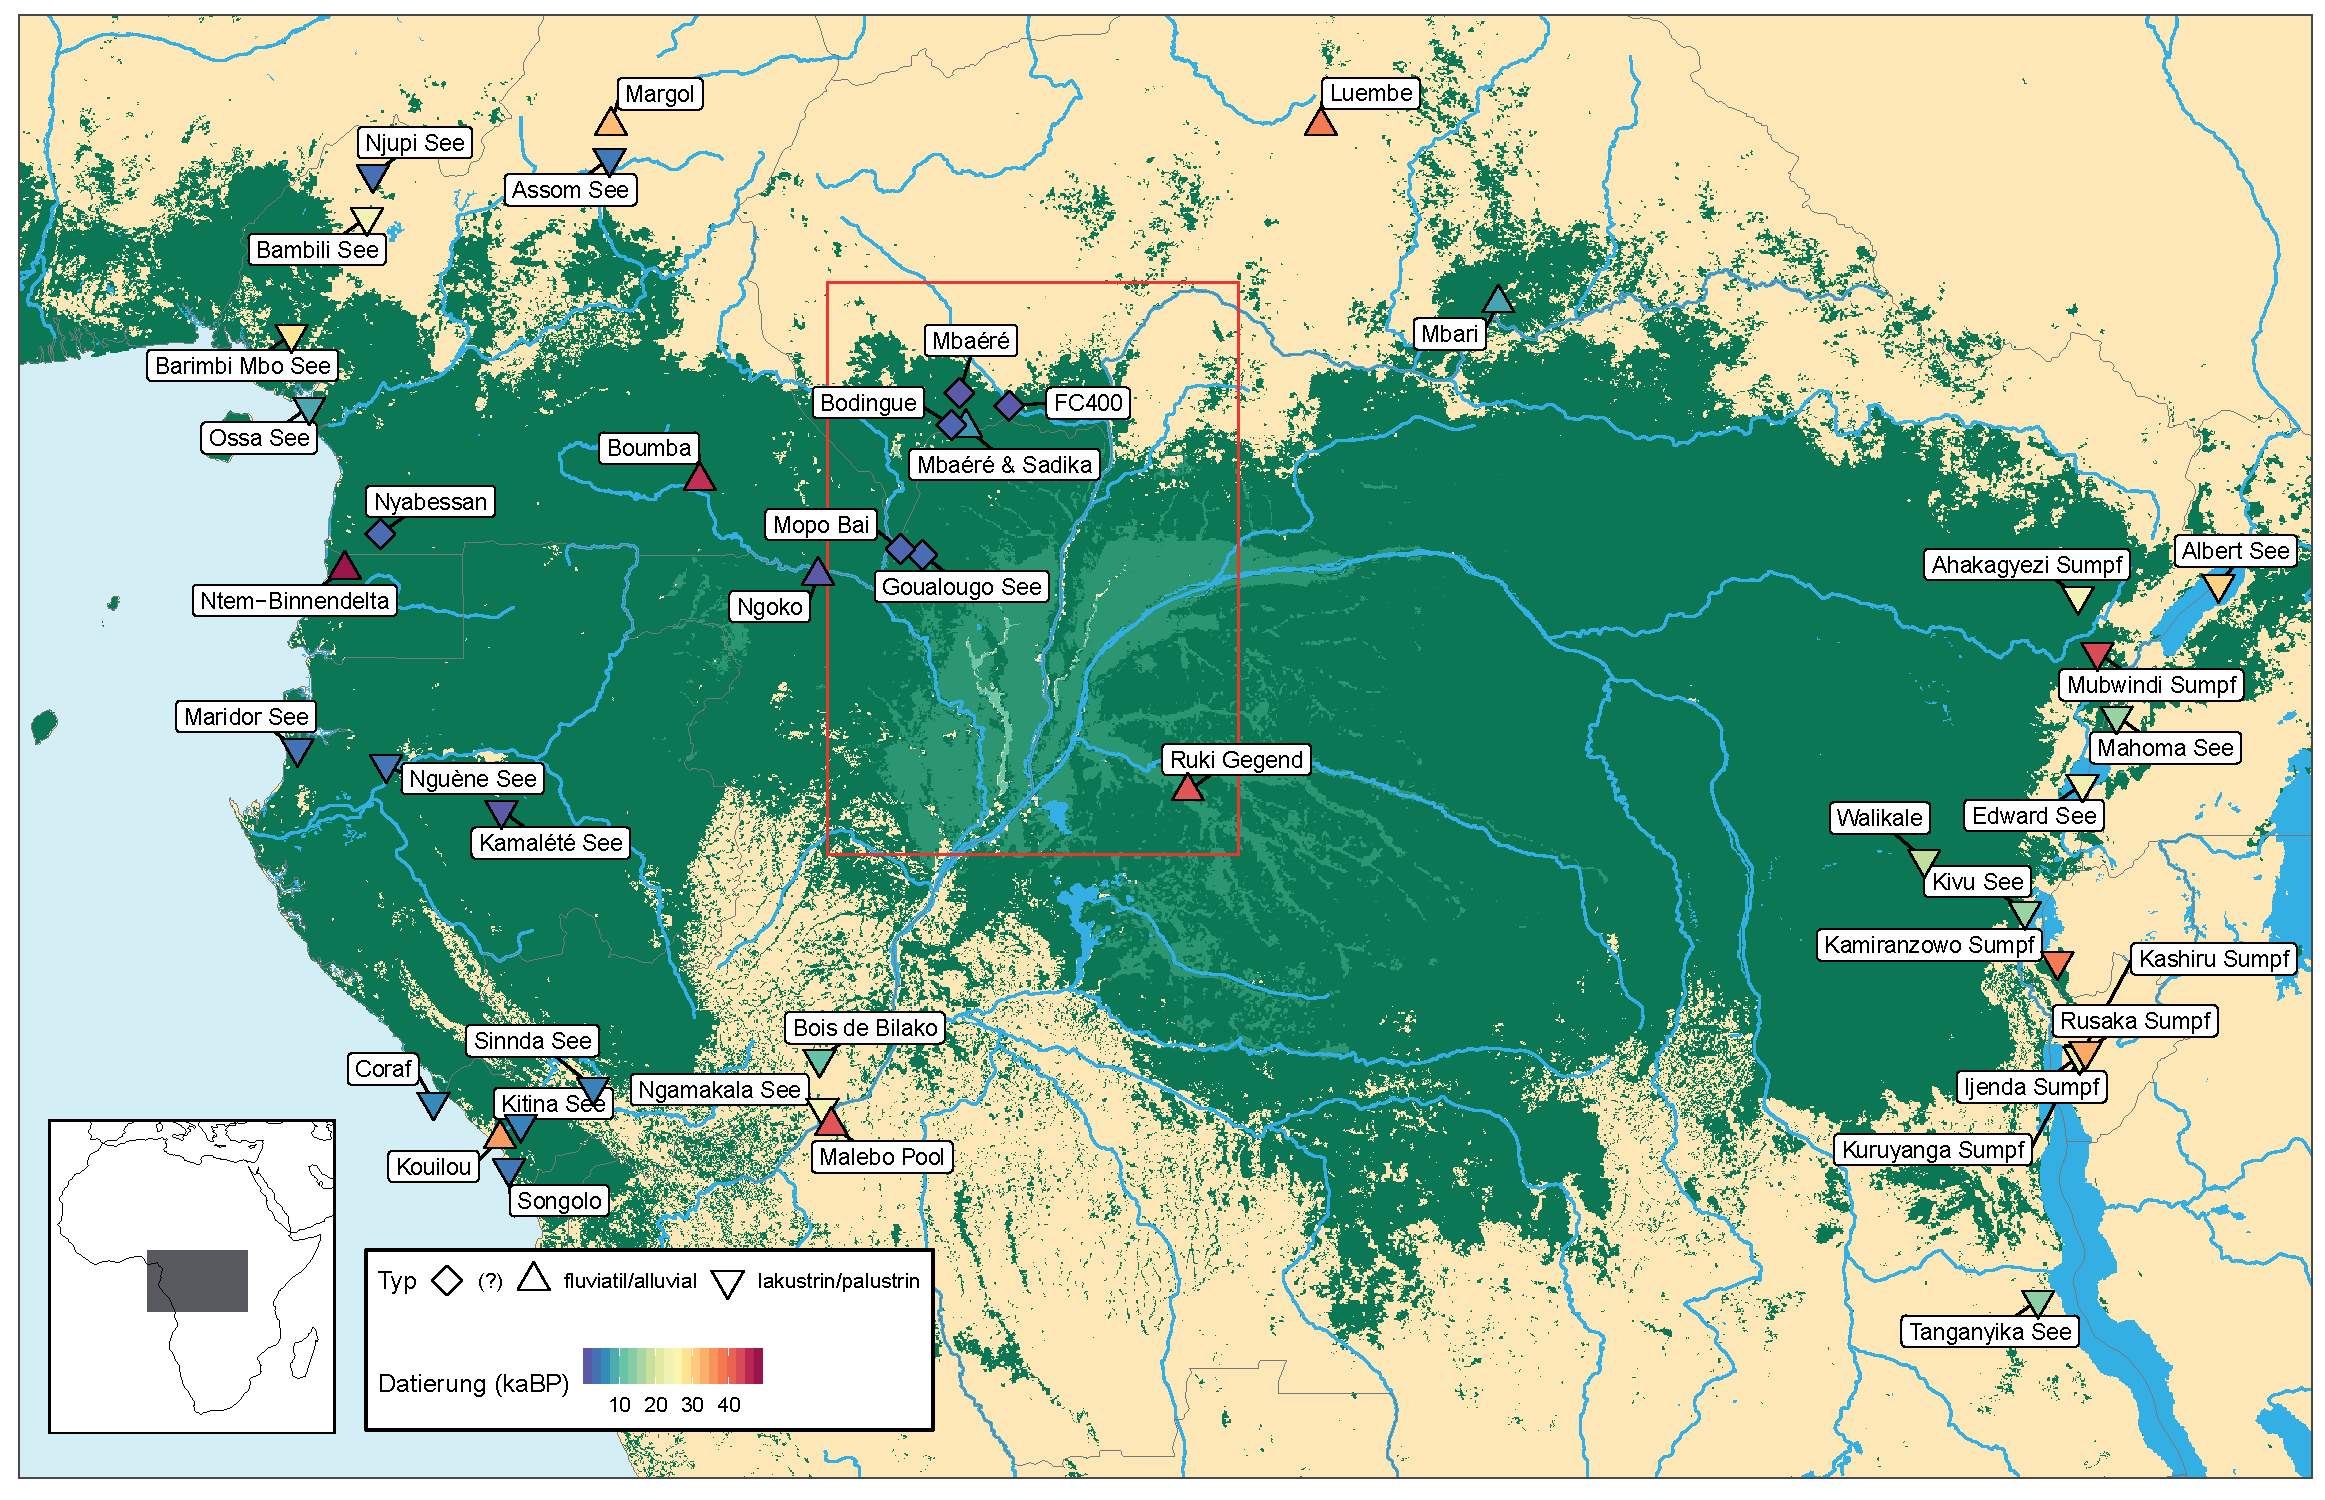
\includegraphics[width=\textwidth]{fig/Ch1_Fig2_PalaoUmwelt.pdf}
	\caption{Paläo-Umweltarchive und Vegetation: Kartierung der wichtigsten lakustrinen und palustrinen sowie fluviatilen und alluvialen Paläo-Umweltarchive sowie das maximale Alter der Ablagerungen \parencites[nach][]{Brncic.2007}{Brncic.2009}[43 Abb.~16, 46 Abb.~17]{Sangen.2009}{Kiahtipes.2011}{Kiahtipes.2016}. Rezente Verbreitung des immergrünen tropischen Regenwaldes (dunkelgrün) sowie Sumpfwald (hellgrün) nach \textcite{Mayaux.2003}. Das Arbeitsgebiet ist in rot hervorgehoben (siehe Abb.~\ref{fig:ArbeitsgebietKarte}).}
	\label{fig:PalaeoumweltArch_Karte}
\end{figure*}

Die Sichtweise, dass der tropische ombriophile Regenwald ein statisches Landschaftselement sei, konnte durch neuere Forschungen revidiert werden \parencite[83]{Runge.2001}. Es zeigte sich, dass der komplette Regenwald innerhalb von 40--100 Jahren durch einen komplexen Prozess kreislauforientierter Biomasseumsätze abgebaut und erneuert werden kann. Der immergrüne Regenwald des Inneren Kongobeckens bildet sich ab etwa 1600\,mm mittleren Jahresniederschlags aus (ebd. 83). Während der Waldbestand auf den Grundgebirgs-Latosolen im Randbereich homogen ist, zeigten sich im saisonal überfluteten Zentrum des Kongobeckens stärker heterogene Arten-Zusammensetzungen (ebd. 83\,f.). Die tropischen Wälder müssen folglich als \enquote{entwicklungsgeschichtlich und vom Standort abhängige, differenzierte Ökosysteme} (ebd. 92) betrachtet werden.

Beruhend auf der rezenten Variabilität des Baumartenbestandes wurde von \textcite{Maley.2001} die Ausdehnung des westlichen zentralafrikanischen Regenwaldes im ersten vorchristlichen Jahrtausend rekonstruiert. Diese zeigt ein zum heutigen Stand deutlich reduziertes und auf sogenannte \enquote{Refugien} begrenztes Verbreitungsbild. Die Nordgrenze der von \textsc{Maley} (ebd. 7 Abb.~4) postulierten Regenwaldverbreitung im Bereich des Laufs des \mbox{Ubangi} lag mutmaßlich deutlich südlich von Bangui (Fpl.~215) im Bereich zwischen Imese (Fpl.~201) und Dongo (Fpl.~202). Durch die ebenfalls postulierte Unterbrechung der Regenwaldverbreitung im Gebiet des \mbox{Sangha}, dem sogenannten \enquote{\mbox{Sangha}-Korridor}\footnote{Der auch \enquote{\mbox{Sangha}-Intervall} genannte Bereich beschreibt eine Zone zwischen 14--18$^\circ$~O, in der auffällige Pflanzengemeinschaften beobachtet werden können, die nicht zu den heutigen klimatischen Rahmenbedingungen der Region passen \parencite{Gond.2013}. Zu diesen Auffälligkeiten zählen die Anwesenheit der senegalesischen Dattelpalme (\textit{Phoenix reclinata}), die nirgends sonst im Regenwald beobachtet werden kann. Andererseits fehlen in dieser Region auch einige, für den äquatorialen Regenwald weiter westlich wie östlich charakteristische Pflanzen \parencite[356\,f.]{Bostoen.2015}. Entsprechende Beobachtungen ließen bereits \textcite{Letouzey.1968} eine potenzielle Verbindung zwischen dem nördlichen und südlichen Savannengürtel postulieren.\label{ftn:SanghaIntervall}} \parencites[siehe][]{Russell.2014}{Bostoen.2015} soll sich eine Grenze der Regenwaldverbreitung südlöstlich von Ouesso (Fpl.~265) ergeben haben.

Im engeren Arbeitsgebiet kamen in den letzten Jahren einige Paläo-Umweltarchive hinzu \parencites[siehe][]{Brncic.2007}{Brncic.2009}{Kiahtipes.2011}{Kiahtipes.2016}. Archive sind auch aus Kamerun, Gabun und dem Mündungsgebiet des Kongo bekannt \parencite[siehe][41--58; Abb.~\ref{fig:PalaeoumweltArch_Karte}]{Sangen.2009}. Während es im westlichen Zentralafrika\footnote{Gemeint sind hier die Staatsgebiete von Kamerun und Gabun sowie der Bereich der Kongomündung.} sowie im östlichen Zentral- und in Ostafrika -- vornehmlich in der Region der großen ostafrikanischen Seen -- eine Vielzahl von lakustrinen und palustrinen Paläo-Umweltarchiven gibt, liegen aus dem Kongobecken keine entsprechenden Archive vor (ebd. 54 Abb.~16). Mit Blick auf die fluvialen und alluvialen Paläoumweltarchive sieht die Situation insofern besser aus, als hier die Arbeiten von Johannes \textcites{Preu.1986}{Preu.1986b}{Preu.1990} im Bereich des Ruki genannt werden können. Weitere Untersuchungen fanden am Rand des Kongobeckens in einem Talabschnitt des Mbaéré im Südwesten der Zentralafrikanischen Republik statt \parencite{Neumer.2007}.

Die Rekonstruktion extralokaler Einflüsse auf die Ökologie aus punktuellen Ergebnissen und regionalen Vergleichen bildet eine der grundlegenden Schwierigkeiten für physiogeografische und umweltgeschichtliche Untersuchungen \parencite[42]{Sangen.2009}.\footnote{Die jüngste Phase der Erforschung der Landschaftsgeschichte Zentralafrikas wird von modernen Fernerkundungsverfahren bestimmt \parencite[6]{Runge.2001}. Die grundsätzlich schlechten Erhaltungsbedingungen für Pollen in den für gewöhnlich groben und stark oxidierten meso- bis cenozoischen Ablagerungen des Kongobeckens erschweren palynologische Studien. Als Folge verschob sich der Fokus paläoklimatologischer Untersuchungen in den Bereich geochemischer Analysen und der Untersuchung der sub-marinen Ablagerungen des Kongo-Schwemmkegels \parencite[312]{Giresse.2005b}. Die Turbidit-Ablagerungen im Kongo-Canyon sind ein direktes Resultat der Suspensionsfracht des Kongo und repräsentieren dessen Schwankungen im Zusammenhang mit Faktoren wie Meeresspiegelschwankungen, Tektonik und Klimaveränderungen \parencite[2176]{Savoye.2009}.} Für den Gegenstand dieser Arbeit sind vornehmlich die Einflüsse des Ökosystems und dessen Veränderungen auf die menschliche Besiedlung des Kongobeckens von Bedeutung. Aus dem tropischen Afrika liegen insgesamt nur sehr wenige komplette, vom Ende der letzten Eiszeit bis in die Gegenwart reichende Pollenprofile vor \parencite[2682]{Lezine.2013}, so zum Beispiel das Profil aus dem Sacred Lake in Kenia \parencite[65--73; Beilage Fig.~15]{Coetzee.1967} sowie jenes aus dem Barombi-Mbo-See in Kamerun \parencite{Maley.1991}. Für das Pleistozän im Inneren Kongobecken liegen lediglich vorläufige Untersuchungsergebnisse aus Analysen durch Emile Roche vor, wonach Pollen aus der Ruki- und Momboyo-Region auf eine offene Savannen-Landschaft sowie nahe Marsch-Areale und Galleriewälder hinweisen würden \parencite[181]{Fiedler.1985}.\footnote{Für die Untersuchung wurden organisch reiche Sedimentschichten aus Imbonga am Momboyo \parencite[siehe][542\,f. Karte~1 Fpl.~43]{Wotzka.1995} sowie Bokuma-Isoko am Ruki (Fpl.~18) analysiert, welche zwischen 25\,000--15\,000 bp datieren \parencite[182]{Fiedler.1985}. Eine direkte Publikation dieser Daten liegt nicht vor.}

Eines der aussagekräftigsten Paläo-Umweltarchive, durch das eine Rekonstruktion der Klimaentwicklung der Großregion möglich wird, stammt aus dem knapp 2\,km großen, nahezu kreisrunden und 110\,m tiefen Vulkansee Barombi Mbo in Westkamerun \parencite[159--161]{Maley.1998b}.\footnote{Der in der Seemitte genommene, 23,5\,m lange Sedimentkern BM-6 enthielt Schichten, die zirka 27\,500 Jahre zurückreichen, wobei die untersten 1,5\,m des Kerns eine, vermutlich durch vulkanische Aktivität verursachte, gestörte Lagerung aufwiesen \parencite[6 Abb. 1]{Maley.2001}. Auch aufgrund der allgemeinen Schwierigkeiten einer \textsuperscript{14}C-Datierung in diesen Zeiträumen werden die ältesten ansprechbaren Schichten auf vor 24\,000 Jahren datiert. Die Daten zeigen im für diese Arbeit wichtigen 1.~Jt. v.~Chr. einen Rückgang der Regenwald-Flora beziehungsweise Baumpollen zugunsten von Savannen-Taxa  \parencites[6 Abb. 1]{Maley.2001}[56--58]{Maley.2003}.} Mit Blick auf die Erkenntnisse aus dem Barombi Mbo-Kern wurden von \textcite[357--360]{Schwartz.1992} erstmals Überlegungen zu den Zusammenhängen zwischen der Aufsiedlung des zentralafrikanischen Regenwaldes durch keramikproduzierende und sesshaftlebende Gruppen in der zweiten Hälfte des 1.~Jt. v.~Chr., der Ausbreitung der Eisenmetallurgie in den letzten Jahrhunderten vor der Zeitenwende sowie der heute unter den Begriffen \textit{First Millennium BC Crisis} \parencite[63]{Sangen.2009} beziehungsweise \enquote{Krise des Regenwaldes} \parencite{Neumann.2014} bekannten klimatischen sowie damit einhergehenden ökologischen Veränderung des Regenwaldes nach etwa 1000 v.~Chr. angestellt.

Die Veränderung der Regenwald-Vegetation im 1.~Jt. v.~Chr. lässt sich auch im Pollenprofil aus dem Nyabessan-Sumpf im Ntem-Binnendelta in Südkamerun nachvollziehen \parencite[316]{Ngomanda.2009}. So zeichnet sich gegen 500 v.~Chr. in den Daten ein deutlicher Wandel der Regenwaldflora ab. Das zirka 1,8\,m mächtige und vom 13./11. bis in das 5./3.~Jh. v.~Chr. datierende Profil zeigt für die zweite Hälfte des 1.~Jt. v.~Chr. einen Rückgang des Sekundärwaldes zugunsten eines Anstiegs von Primärwald-Taxa \parencite[ebd. 311 Abb.~3; ][58 Abb.~5]{Neumann.2012}.

Daten für die holozäne Klimageschichte des Arbeitsgebietes liegen aus dem südlichen Teil des \enquote{Nouabalé-Ndoki National Park}, in der nördlichen Republik Kongo vor \parencite{Brncic.2007}.\footnote{Ein etwa 68\,cm langer Sedimentkern aus dem Goualougo-See deckt die letzten 3300~Jahre ab (\textsc{Brncic, Willis} u.~a. 2007: 236--237 Abb.~59). Die Untersuchung ergab, dass sich überregionale klimatische Vorgänge kaum niedergeschlagen haben, da feuchte semi-immergrüne Waldtaxa durch die gesamte, durch den Kern abgedeckte Zeit hindurch konstant vorkamen (ebd. 240). Anzeichen für eine Savannen-Ausbreitung konnten nicht beobachtet werden. In den vergangenen 1000 Jahren mehren sich Anzeichen für anthropogene Feuer. Verschiedene Pioniertaxa wie \textit{E. guineensis}, \textit{Tetrorchidium} sp. und \textit{Erythrophleum} sp. zeigen trockenere Perioden an (ebd.). Das Vorkommen dieser Taxa ist fast ausschließlich auf das 1.~Jt. v.~Chr. beschränkt (ebd. 236 Fig.~5).} Der anthropogene Einfluss auf die Vegetation der Region innerhalb der letzten 3000~Jahre ist demnach größer als jener der auf klimatische Veränderungen zurückgeht. Ein zweiter Sedimentkern stammt aus Mopo Bai, einer saisonal überfluteten, sumpfigen Niederung etwa 28\,km westnordwestlich des Goualougo-Sees \parencite[80]{Brncic.2009}. Der 1\,m lange Kern deckt die letzten 2500~Jahre ab und die Pollensequenz zeigt deutliche Einflüsse klimatischer und anthropogener Faktoren auf die Ökologie (ebd. 86). Die Holzkohlekonzentration nimmt ab dem 11.~Jh. n.~Chr. in Form mehrerer, ansteigender Spitzenwerte zu (ebd. 85 Abb.~5) und der Anteil von \textit{Elaeïs guineensis} -- einer Pioniertaxa -- ist um die Zeitenwende am größten und nimmt ab dann stetig ab (ebd. 83 Abb.~4).

Aus dem Ngotto-Waldschutzgebiet im äußersten Südwesten der Zentralafrikanischen Republik ist die Untersuchung von zwei Pollenkernen bekannt \parencite{Kiahtipes.2011}. Ein Sedimentkern wurde 2007 aus der Flussmarsch des Bodingue gezogen.\footnote{Der insgesamt 72\,cm lange Kern wurde in Abständen von 10\,cm beprobt. Drei aus dem oberen, mittleren und unteren Bereich des Kerns genommene \textsuperscript{14}C-Proben zeigen an, dass er eine Zeitspanne vom 5.~Jh. v.~Chr. bis zum 13.~Jh. n.~Chr. abdeckt (\textsc{Kiahtipes} u.~a. 2011: 4 Tab.~1; 5 Fig.~2).} Ein zweiter Kern stammt aus der Uferzone der Flussmarsch des Mbaéré.\footnote{Der 2,5\,m lange Kern wurde in Intervallen von 5\,cm beprobt. In die Analyse ging nur jede zweite Probe ein. Der Kern deckt eine Zeitspanne vom 7./8.~Jh. n.~Chr. bis in die Gegenwart ab (\textsc{Kiahtipes} u.~a. 2011: 11 Fig.~6).} Kombiniert bietet sich durch beide Kerne ein Einblick in die regionale Entwicklung für die letzten etwa 2500 Jahre (ebd. 4 Tab.~1, 5 Fig.~2). Nahe des Zusammenflusses der Flüsse Loame und Lobaye wurde in einer Region mit Feuchtsavannen-Vegetation ein 2\,m langer Sedimentkern erbohrt \parencite[5]{Lupo.2015}. Radiokohlenstoffdatierungen zeigten, dass der Kern Paläo-Umweltdaten der letzten 500 Jahre abdeckt (ebd. 13 Abb.~6). In der Auswertung zeigte sich ein Wechsel von einer dichten Regenwaldvegetation zu einer offeneren, savannenartigeren Vegetation im späten 17. oder frühen 18.~Jh.
\end{multicols}
\chapter{Quellen und Methoden}\label{sec:Quellen}
\begin{multicols}{2}
\raggedcolumns
\noindent Das im Rahmen dieser Arbeit bearbeitete Quellenmaterial umfasst 10\,519 Fundstücke von 122 individuellen Fundplätzen in einem 500\,$\times$\,700\,km großen Arbeitsgebiet (Kap.~\ref{sec:Arbeitsgebiet}). Das Material stammt zu einem großen Teil aus 143 individuellen Oberflächenabsammlungen.\footnote{Während an allen Fundstellen mindestens die moderne Dorffläche nach Funden wie Befunden abgesucht wurde, existieren von einigen Plätzen Komplexe aus zusätzlichen, spezifischen Bereichen (siehe Katalog B).} Eine belastbare Quellenbasis bildeten 13 ausgegrabene sowie sechs weitere, zwar als Befunde erkannte, aber nicht systematisch untersuchte Komplexe (Tab.~\ref{TabBefundeUntersucht}). Da keine exakten geografischen Koordinaten der Fundstellen bekannt waren, mussten diese nachträglich ermittelt werden.\footnote{Die Fundstellen wurden während der Befahrung der Flüsse in Flussatlanten, welche von der staatlichen, damals za{\"i}rischen Transport- und Schifffahrtsbehörde ONATRA (\textit{Office national des Transports}) stammten, verzeichnet. Die Erhebung der Koordinaten erfolgte durch Abgleich dieser um entsprechende Notizen ergänzten Flussatlanten mit GoogleEarth-Satellitendaten. Diese Vorgehensweise bedingt eine gewisse Unschärfe der ermittelten Positionen, da es von Fall zu Fall kleinere Unterschiede im Kartenmaterial gab. Die Positionen der Fundstellen innerhalb der Ortschaften ließ sich regelhaft nicht mehr präzise rekonstruieren. Die in GoogleEarth ermittelten Koordinaten für die Fundstellen wurden in Dezimalgrade umgerechnet und als Längen- sowie Breitenangabe aufgenommen (Anlage 1.B).} Die Vergabe von Katalognummern, im weiteren als \enquote{Fpl.} abgekürzt, schließt an den 185 Fundstellen umfassenden Katalog von \textcite[542\,f. Karte 1]{Wotzka.1995} an.

Die Aktenlage umfasste neben der ursprünglichen Dokumentation\footnote{Aufgrund des zeitlichen Abstandes zwischen den Feldarbeiten des \textit{River Reconnaissance Project} in den 1980er Jahren und der aktuellen Aufarbeitung konnten offene Fragen an die ursprüngliche Dokumentation nicht immer zufriedenstellend geklärt werden. Als zentrales Problem erwies sich das Fehlen der schriftlichen Felddokumentation von Célestin Kanimba Misago, dem damaligen Mitarbeiter der \textit{Musées Nationaux du Zaïre} (heute \textit{Institut des Musées Nationaux du Congo}) in Kinshasa und Kooperationspartner. Während die Feldbücher der übrigen Teilnehmer der Reisen von 1985 und 1987 im Original wie in Kopie vorlagen, konnten jene von Kanimba Misago nicht aufgefunden werden. Während der Kampagne von 1987 hatte Kanimba Misago die Komplexe BBS~87/1 (Kat.-Nr.~6) in Bobusa am unteren \mbox{Sangha} (Fpl.~239) und PIK~87/3 (Kat.-Nr.~10) in Pikunda am mittleren \mbox{Sangha} (Fpl.~255) ausgegraben. Der Metallurgie-Befund PIK~87/3, welcher nach Ausweis der vorliegenden Radiokohlenstoffdatierung in das 11.--13.~Jh. n.~Chr. (Abb.~\ref{fig:PIK87_Datierungen}) datiert und damit einer der ältesten Belege für einen flachen, offenen Ofen mit Schlackeabfluss in der Region darstellt, konnte ausschließlich auf einer nur bedingt systematischen fotografischen Dokumentation sowie einer Kurzbeschreibung durch \textsc{Kanimba Misago} aus dem Jahr 1995 beschrieben werden (Details siehe Kat.-Nr.~10), was bei der Bedeutung des Befundes bedauerlich ist.}, die im Gelände angefertigt wurde, auch eine Reihe von internen Berichten und Teile unveröffentlichter Manuskripte. Wo diese für die Aufarbeitung des Materials herangezogen wurden, sind sie entsprechend als Quelle im Text ausgewiesen. Die in dieser Arbeit durchgeführten Analysen gründen sich in allen Fällen auf den eigenen Beobachtungen des Autors am Fundmaterial sowie der Auswertung der im Gelände angefertigten Dokumentation (Katalog~A).

\section{Surveys, Grabungen und Befunde}\label{sec:GrabungenBefunde}

\subsection{Grubenbefunde}

In die Auswertung flossen 13 Grabungsbefunde von fünf verschiedenen Fundstellen ein sowie sechs Komplexe, die zwar einen klaren Befundcharakter aufweisen, aber nicht systematisch ergraben wurden (Tab.~\ref{TabBefundeUntersucht}, Katalog A). Zu letzterer Gruppe werden zum Beispiel die Komplexe MLB~85/103 (Kat.-Nr.~5) und LKW~87/186 (Kat.-Nr.~19) gerechnet, die zwar eindeutig als Gruben angesprochen werden können, jedoch nicht ausgegraben wurden. Da sich diese Beobachtungen aber aufgrund ihrer Geschlossenheit grundsätzlich von den ebenfalls in die Gesamtauswertung eingeflossenen Surveyfunden (Katalog B) unterscheiden, werden sie gemeinsam mit den Grabungsbefunde besprochen.

\begin{table*}[!t]
\centering
%\resizebox{\textwidth}{!}{%
{\footnotesize
\begin{sftabular}{@{}lllll@{}}
\toprule
\textbf{Fundstelle} & \textbf{Gruben} & \begin{tabular}[c]{@{}l@{}}\textbf{Metallurgie-}\\ \textbf{befunde} \end{tabular} & \textbf{Gräber} & \begin{tabular}[c]{@{}l@{}}\textbf{Schichten-}\\ \textbf{Abfolge} \end{tabular} \\
\midrule
\begin{tabular}[c]{@{}l@{}}\textbf{Maluba}\\(Fpl.~230)\end{tabular} & \begin{tabular}[c]{@{}l@{}}MLB 85/1-3-1\\ MLB 85/1-3-2\\ (MLB 85/2)\\ (MLB 85/103)\end{tabular} & & MLB 85/1-4-3 & \\ %\hdashline
\begin{tabular}[c]{@{}l@{}}\textbf{Bobusa}\\(Fpl.~239)\end{tabular} & & & & \begin{tabular}[c]{@{}l@{}}BBS 87/1\\ BBS 87/2\end{tabular} \\[3ex] %\hdashline
\begin{tabular}[c]{@{}l@{}}\textbf{Pikunda}\\(Fpl.~255)\end{tabular} & \begin{tabular}[c]{@{}l@{}}PIK~87/1\\ PIK~87/2\end{tabular} & PIK~87/3 & & \\[3ex] %\hdashline
\begin{tabular}[c]{@{}l@{}}\textbf{Ngombe}\\(Fpl.~252)\end{tabular} & (NGO~87/102) & & & \\[3ex] %\hdashline
\begin{tabular}[c]{@{}l@{}}\textbf{Mitula}\\(Fpl.~251)\end{tabular} & (MIT~87/103) & & & \\[3ex] %\hdashline
\begin{tabular}[c]{@{}l@{}}\textbf{Mobaka}\\(Fpl.~246)\end{tabular} & (MKA~87/102) & & & \\[3ex] %\hdashline
\begin{tabular}[c]{@{}l@{}}\textbf{Boleko}\\(Fpl.~285)\end{tabular} & & & BLK 87/1 & \\[3ex] %\hdashline
\begin{tabular}[c]{@{}l@{}}\textbf{Likwala Fluss-}\\ \textbf{Kilometer~186}\\(Fpl.~291)\end{tabular} & (LKW~87/186-1) & & & \\[3ex] %\hdashline
\begin{tabular}[c]{@{}l@{}}\textbf{Munda}\\(Fpl.~304)\end{tabular} & \begin{tabular}[c]{@{}l@{}}MUN~87/2-1-1 A \\ MUN~87/2-1-3\end{tabular} & \begin{tabular}[c]{@{}l@{}}MUN~87/1 \\ MUN~87/2-1-1 B/C \\ MUN~87/3\end{tabular} & & \\
\bottomrule
\end{sftabular}}
%}
\caption{Ausgegrabene Befunde: Übersicht über die untersuchten Befunde im Arbeitsgebiet aufgeteilt nach Befundkategorien. Die in Klammern stehenden Komplexe wurden nicht systematisch ausgegraben, aber als Befunde erkannt. Die Sortierung der Liste orientiert sich an der Abfolge, in der die Befunde untersucht wurden.}
\label{TabBefundeUntersucht}
\end{table*}

Im Jahr 1985 wurden bei der Befahrung der Flüsse \mbox{Ubangi} und Lua lediglich in Maluba am Lua (Fpl.~230, Kat.-Nr.~1--5) Grabungen durchgeführt. Von den insgesamt vier dort beobachteten Gruben wurden nur zwei vollständig untersucht und dokumentiert (Kat.-Nr.~1--2). Die ursprüngliche Verfüllung einer weiteren Grube (Kat.-Nr.~4) stürzte während der Grabung ein. Daher wurde der Befund nicht mehr weiter untersucht. Es wurden auch keine Funde dieses Befundes geborgen beziehungsweise zur Auswertung lagen keine Funde aus dieser Grube mehr vor. Eine vierte Grube (Kat.-Nr.~5) ist zwar als solche zu erkennen gewesen, es wurde aber lediglich eine geringe Menge keramischen Fundgutes entnommen und keine Grabung durchgeführt. Während der Kampagne von 1987 im nördlichen Teil der Republik Kongo, entlang der Flüsse \mbox{Sangha}, \mbox{Ngoko} und Liwkala-aux-Herbes sowie eines kurzen Abschnitts des Kongo, wurden zehn Befunde an vier verschiedenen Fundstellen untersucht. In Pikunda am mittleren \mbox{Sangha} (Fpl.~255) wurden an zwei benachbarten Grabungsstellen insgesamt drei Gruben (Kat.-Nr.~8--9) erfasst. In Munda am \mbox{Likwala}-\mbox{aux}-\mbox{Herbes} (Fpl.~304) fanden die umfangreichsten Ausgrabungen des \textit{River Reconnaissance Project} im Arbeitsgebiet statt. Innerhalb eines eng begrenzten Areals wurden vier Komplexe näher untersucht, die drei Gruben sowie drei Verhüttungsbefunde erbrachten. Die Grabungen MUN~87/1 (Kat.-Nr.~15) sowie MUN~87/2--1--1 (Kat.-Nr.~16) ergaben jeweils eine Grube sowie einen Verhüttungsbefund, während es sich bei Befund MUN~87/2--1--3 (Kat.-Nr.~17) um eine weitere Grube handelt.

Für das \mbox{Sangha}- und Likwala-aux-Herbes-Gebiet lassen sich auf Basis der ausgegrabenen Befunde in Pikunda (Fpl.~255) und Munda (Fpl.~304) Grundlagen der chronologischen Sequenz erarbeiten (siehe Kap.~\ref{sec:SequenzLikwala}--\ref{sec:SequenzSanghaNgoko}). Die Grabungen in Maluba am Lua (Fpl.~230) decken nur eine der belegten keramischen Stilgruppen ab und ermöglichen kaum weiterführende Aussagen zum Ablauf der Besiedlung im \mbox{Ubangi}- und Lua-Gebiet. Zwar liefern die Funde aus ausgegrabenen Kontexten oder eindeutig ansprechbaren Befunden die beste Datenlage, jedoch spiegeln sie nur sehr begrenzte Nutzungsphasen innerhalb der jeweiligen Fundstelle wider.

In Zentralafrika sind Grundbefunde die am häufigsten dokumentierte Befundkategorie und auch im Arbeitsgebiet wurden vor allem Gruben untersucht. Die Frage nach der Bedeutung dieser Befunde -- ihre Nutzung und Funktion in der Vergangenheit -- ist Gegenstand einer anhaltenden Diskussion \parencite[siehe][197--199]{Meister.2008b}. Während Merkmale wie die häufig in den Befunden beobachtete fragmentierte Gefäßkeramik sowie botanische Reste vordergründig eine profane Nutzung nahelegen, deuten andere Eigenschaften andere Verwendungen an. Der bislang ambitionierteste Interpretationsansatz stammt von \textcite{Wotzka.1993} und gründet auf die Feldarbeit des \textit{River Reconnaissance Project} sowie einem detaillierten Survey ethnologischer Literaturbelege. Die von Wotzka bearbeiteten 34 Grubenbefunde des Inneren Kongobeckens und die dabei beobachteten Deponierungen von Gefäßkeramik in ihnen bildeten die Grundlage für seine Auseinandersetzung mit der Frage nach der Funktion von Keramikdeponierungen in Gruben im zentralafrikanischen Regenwald. \textsc{Wotzka} (ebd. 262\,f. Tab.~1) stellte die an den Grubenbefunden beobachteten Merkmale zusammen und beschrieb sie im Sinne einer polythetischen, sich aus überschneidenden Typen zusammensetzenden Gruppe \parencite[siehe][37\,f. mit Abb.~3]{Clark.1968}. Aus archäologischer Perspektive kann er deutlich machen, dass es sich bei den von ihm untersuchten Befunden nicht um reine \mbox{Abfall-,} Vorrats-, Lehm- oder Lateritentnahmegruben handelt \parencite[264]{Wotzka.1993}. In der von ihm gesichteten ethnographischen Literatur berücksichtigte er auch an Gefäßkeramik aus Gruben beobachtbare Modifikationen oder intentionellen Zerstörungen von Böden oder Appliken (ebd.~262\,f. Tab.~1 Merkmale 6, 13 und 15). In seiner abschließenden Bewertung steht für \textsc{Wotzka} (ebd. 272) die \enquote{Erkenntnis, dass es zahlreiche in rezenter und subrezenter Zeit beobachtete Belege für rituelle Zerstörung von Keramik und anderen Sachgütern gibt, die in einem allgemeinem Zusammenhang mit dem Totenkult stehen}.\footnote{Erste geochemische Untersuchungen von Grubensedimenten aus Fundstellen in Südkamerun offenbarten eine Anreicherung von Phosphat im Bereich der Grubensohlen \parencites[722--724]{MbidaMindzie.19951996}{MbidaMindzie.1998}[147--150; 151--155]{Eggert.2016}. Während \textcite[209]{MbidaMindzie.1998} die auffällige Phosphatanreicherung, die in drei Gruben der Fundstelle Nkang beobachtet wurde, mit anthropogenen Faktoren in Verbindung bringt, weisen \textcite[151--155]{Eggert.2016} auf die Nichtberücksichtigung einer durch die niedrigen ph-Werte möglichen natürlichen Akkumulation hin. Im Zuge der vorliegenden Untersuchung wurde die Fragmentierung der in den Grubenbefunden des Arbeitsgebietes angetroffenen Gefäßkeramik dezidiert aufgenommen (siehe Abb.~\ref{fig:Fragmenierung_MLB85-131}, \ref{fig:Fragmenierung_MLB85-132}, \ref{fig:Fragmenierung_BBS87-1}, \ref{fig:Fragmenierung_BBS87-2}, \ref{fig:PIK87-1_Fragmentierung}, \ref{fig:BLK87-1_Keramik_Fragm}, \ref{fig:MUN87-1_Fragmentierung}, \ref{fig:MUN87-211_Fragmentierung}, \ref{fig:MUN87-213_Fragmentierung}). Während diese Verteilungen zwischen den verschiedenen Formen von Gruben und generell zwischen den Befundkategorien deutlich voneinander abwichen, steht eine spezifische Diskussion der daraus abzuleitenden Schlüsse noch aus.\label{ftn:GeochemieGruben}} Eine universelle Ansprache der Nutzung und Funktion von Gruben in Zentralafrika ergibt sich auch durch die Studie Wotzkas nicht, jedoch erweitert sie den Interpretationsansatz über allzu simple, profane Nutzungsmuster hinaus um eben jene sozialen Komponenten, die Gruben und vor allem die charakteristischen Deponierung von Gefäßkeramik als Teil des Alltags der prähistorischen Gesellschaften Zentralafrikas interpretierbar machen. Weiterhin muss jeder Befund individuell angesprochen und auf seine Genese hin untersucht werden.\footnote{Der Wandel von Nutzungsmustern über die Dauer des Bestehens eines Befundes lässt sich in geradezu exemplarischer Weise am Befund MUN~87/2-1-1 (Kat.-Nr.~16) in Munda am oberen \mbox{Likwala}-\mbox{aux}-\mbox{Herbes} (Fpl.~304) ablesen.}


\subsection{Sonstige Befunde}

Neben den Gruben zählen zu den archäologisch untersuchten Befunden im Arbeitsgebiet noch vier weitere Strukturen, die mit Eisenerzverhüttung in der Region in Zusammenhang gebracht werden können (Tab.~\ref{TabBefundeUntersucht}). Einer dieser Befunde wurde in Pikunda am \mbox{Sangha}, zusätzlich zu den genannten Gruben, als dritte Grabungsstelle erfasst (Kat.-Nr.~10). Die drei übrigen Befunde dieser Kategorie wurden ebenfalls 1987 bei den Ausgrabungen in Munda am \mbox{Likwala}-\mbox{aux}-\mbox{Herbes} untersucht. Neben den in den beiden Grabungsstellen MUN~87/1 (Kat.-Nr.~15) sowie MUN~87/2-1-1 (Kat.-Nr.~16) erfassten Verhüttungsstrukturen wurde in unmittelbarer Nähe ein weiterer Ofenbefund beobachtet und unter der Befundnummer MUN~87/3 (Kat.-Nr.~18) untersucht.

Zusätzlich zu den genannten Verhüttungsbefunden wurden zwei Bestattungen erfasst. Bei der Grabung im Jahr 1985 in Maluba am Lua (Fpl.~230) wurde zwischen den beiden ausgegrabenen Gruben (Kat.-Nr.~1--2) eine in einer kleinen Eingrabung angelegte Sekundärbestattung (Kat.-Nr.~3) erfasst und dokumentiert. Ein subrezentes Körpergrab (Kat.-Nr.~14) wurde 1987 in Boleko am \mbox{Likwala}-\mbox{aux}-\mbox{Herbes} (Fpl.~285) archäologisch untersucht.

Zwei zur Erfassung der jeweiligen Schichtabfolgen angelegte Sondageschnitte in Bobusa an der Mündung des \mbox{Sangha} (Fpl.~239) wurden ausgehend von bestehenden Bodeneingriffen angelegt. Sie waren jeweils nur 1\,m\textsuperscript{2} groß und reichten nur bis in etwa 1\,m Tiefe (Kat.-Nr.~6--7).


\subsection{Surveys}

Etwa zwei Drittel der untersuchten Funde stammen von Oberflächenabsammlungen. Zusammengenommen konnten 143 separate Komplexe von 118 Fundstellen herangezogen werden. Da die ausgegrabenen Befunde nur einen ungenügenden Einblick in die chronologischen Relationen zwischen den keramischen Stilgruppen boten und somit eine Rekonstruktion des Besiedlungsganges auf Basis dieser Daten nicht möglich war, musste dem von der Oberfläche der Dörfer abgesammelten Material verstärkt Beachtung geschenkt werden. Die Inventare aus Oberflächenabsammlungen setzen sich im Mittel aus jeweils gerade einmal 40 Fundstücken zusammen. Während die umfangreichsten Komplexe aus bis zu 289 Stücken bestehen, setzt sich die Hälfte aller Oberflächenabsammlungen aus weniger als 22 Fundobjekten zusammen. Neben den grundsätzlichen Schwierigkeiten im Umgang mit Funden aus Oberflächensurveys illustrieren die genannten statistischen Kennzahlen die Probleme bei der quantitativen Auswertung der entsprechenden Komplexe.

Die interne Zusammensetzung von Komplexen aus Oberflächensurveys ist grundsätzlich vielfältigen Parametern unterworfen.\footnote{Die Zusammensetzung eines Komplexes aus einem Oberflächensurvey ist nur zum Teil durch die archäologische sowie geomorphologische Situation an der Fundstelle bestimmt. In den hier zur Untersuchung vorliegenden Funden aus Dörfern im Zentralafrikanischen Regenwald ist aufgrund der gängigen Praxis des Fegens der Dorffläche zur Reinhaltung vor Bewuchs und Kleintieren mit einer großen Verlagerung von Objekten innerhalb der Fundstelle zu rechnen \parencite[355 Anm.~1]{Wotzka.1995}. Darüber hinaus spielen aber auch Faktoren eine Rolle, die mit dem Survey selbst zu tun haben, wie die Witterung, die Nutzung spezifischer Bereiche eines Dorfes zum Zeitpunkt des Surveys und auch die Erfahrung des Sammelnden.} Indizien für eine mögliche Vermischung von Funden ergaben sich im Zuge der Auswertung der Survey-Inventare von zwei im Gelände unterschiedenen Bereichen einer Fundstelle. Im Fall von zwei anderen Inventaren wurde eine Vermischung der Funde bereits 1990 festgestellt.\footnote{Aus Bobusa am unteren \mbox{Sangha} (Fpl.~239) liegen zwei direkt anpassende Scherben eines Reiseherdes vor (siehe Kap.~\ref{sec:Reiseherde}). Während ein Stück im Dorf (BBS~87/101:10) gefunden wurde, stammt eine weiteres, direkt anpassendes Fragment aus der als \textit{elali} (siehe Anm.~\ref{ftn:elali}) bezeichneten Dorfwüstung (BBS~87/102:81). Nach den Angaben im Feldbuch von Manfred Eggerts lag das \textit{elali} etwa 7 Weg-Minuten vom Dorf entfernt. Auf Basis der vorliegenden Unterlagen kann eine simple Verwechslung der Nummerierung bei der Beschriftung der Stücke im Anschluss an die Feldkampagne von 1987 nicht ausgeschlossen werden. Inwieweit eine mögliche Verlagerung der Funde auf natürlichem oder artifiziellem Wege bestehen kann, muss offenbleiben. Das Material des Komplexes NGO~87/101 aus Ngombe am \mbox{Sangha} (Fpl.~252) wurde zu einem nur grob eingrenzbaren Zeitpunkt mit jenem des Komplexes NGL~87/101 aus Ngombe am \mbox{Likwala}-\mbox{aux}-\mbox{Herbes} (Fpl.~283) vermischt. Allen Funden des Komplexes NGO~87/101 wurde die Kennung NGL~87/101 gegeben. Erkannt wurde dieser Umstand erst 1990 von Eggert, als ihm bei einer Durchsicht der Funde der Kampagne von 1987 auffiel, dass \textit{offiziell} keine Funde mit der Kennung NGO 87/101 vorliegen. Im Fall der Scherben aus den beiden Fundstellen muss die Vermischung bereits sehr zeitig, möglicherweise bereits im Feld, bei der Vorbereitung des Exports der Funde oder kurz danach stattgefunden haben. In den verfügbaren Packlisten waren bereits nur die beiden Komplexe NGL~87/101 und NGO~87/102 und kein Komplex NGO~87/101 verzeichnet. Ein entsprechender Komplex ist jedoch eindeutig im Feldbuch Eggerts sowie der Kartei der Fundstellenkürzel mit der Beschreibung \enquote{Dorf allgemein} ausgewiesen. Im Zuge der Aufarbeitung der Funde ergaben sich nur wenige stichhaltige Indizien, die eine Trennung des mit NGL~87/101 beschrifteten Materials, insgesamt 112 Scherben, auf zwei Komplexe ermöglichten. Auffällig ist das Auftreten von rouletteverzierter Keramik, die an Fundstellen entlang des Likwala-aux-Hebers kaum beobachtet wurde (siehe Kap.~\ref{sec:SequenzLikwala}), am \mbox{Sangha} jedoch durchaus vertreten ist (siehe Kap.~\ref{sec:SequenzSanghaNgoko}). Beruhend auf den Inventaren der jeweils benachbarten Fundstellen konnte unter Vorbehalten das jeweilige Ensemble der Stilgruppen an den beiden Fundplätzen rekonstruiert werden (siehe Tab.~\ref{tab:LikwalaSequenz}, \ref{tab:SanghaNgokoSequenz}).\label{ftn:Vermischungen}}

\section{Funde}

Die umfangreichste Fundgattung innerhalb des untersuchten Materials bildet die Gefäßkeramik (Tab.~\ref{tab:Funde_Uebersicht}). Die insgesamt 8469 Gefäßeinheiten und Scherben machen 80\,\% des gesamten Fundgutes aus. Unter den restlichen, nichtkeramischen Funden nehmen Metallurgieüberreste, vor allem Schlacken mit 1321 Stücken beziehungsweise knapp 40\,kg eine hervorzuhebende Stellung ein. Die weiteren Fundkategorien sind häufig nur durch wenige Stücke vertreten.

\begin{figure*}[tb]
\noindent\begin{minipage}[b]{\columnwidth}
	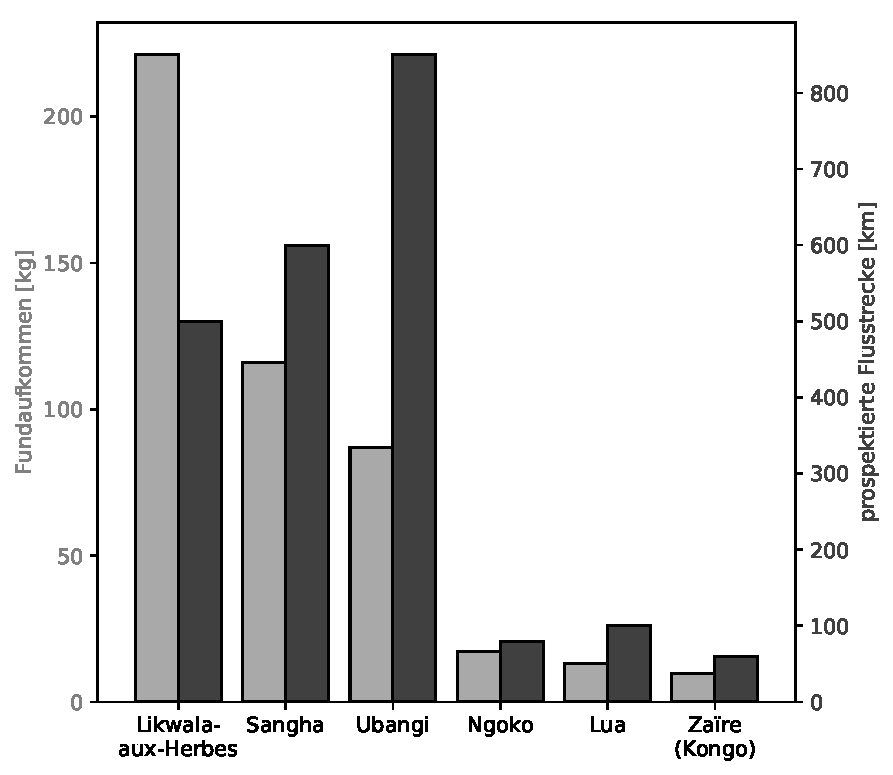
\includegraphics[width=\columnwidth]{fig/2-2_FundeGewicht_FlussKM.pdf}
	\captionof{figure}{Funde: Vergleich des Fundaufkommens (hell) mit Bezug auf die Länge des befahrenen Flussabschnitts (dunkel).\label{fig:FundGewVSFlussKM}}
\end{minipage}\hfill
\noindent\begin{minipage}[b]{\columnwidth}
{\footnotesize \begin{sftabular}{@{}p{.325\columnwidth}R{.125\columnwidth}R{.075\columnwidth}R{.175\columnwidth}R{.075\columnwidth}@{}}
		\toprule
		\textbf{Fundkategorie} &  \textbf{Anzahl} &     \textbf{\%} &  \textbf{Gew. (kg)} &     \textbf{\%} \\
		\midrule
		Gefäßkeramik &    8469 &   80,5 &        363,34 &   78,3 \\
		Schlacke &    1321 &   12,6 &         39,73 &    8,6 \\
		gebrannter Lehm &     187 &    1,8 &          6,25 &    1,3 \\
		Ofenwand &     182 &    1,7 &         19,88 &    4,3 \\
		keram. Sonderform &     117 &    1,1 &         11,19 &    2,4 \\
		Tuyere &      94 &    0,9 &          6,81 &    1,5 \\
		Stein &      76 &    0,7 &          7,23 &    1,6 \\
		Knochen &      29 &    0,3 &          5,93 &    1,3 \\
		Eisen &      13 &    0,1 &          0,53 &    0,1 \\
		Laterit &      11 &    0,1 &          0,08 &    0,0 \\
		Glas &       6 &    0,1 &          0,01 &    0,0 \\
		Metall &       8 &    0,1 &          0,38 &    0,1 \\
		Botanik &       2 &    0,1 &             - &      - \\ 
		Sonstige &       5 &    0,1 &          2,52 &    0,5 \\ \bottomrule			\multicolumn{1}{r}{\textbf{$\sum$}} &   10519 &  100 &        463,88 &  100 \\
		\bottomrule
	\end{sftabular}
}
\captionof{table}{Funde: Übersicht der in die Auswertung eingeflossenen Fundkategorien und ihrer Anteile.\label{tab:Funde_Uebersicht}}
\end{minipage}
\end{figure*}

Die Funde sind, obschon der Geländearbeit innerhalb beider Kampagnen die gleiche Surveystrategie zugrunde lag, nicht gleichmäßig im Arbeitsgebiet verteilt. Während einige Regionen sehr gut repräsentiert sind, liegen aus anderen Räumen nur vergleichsweise wenige Funde vor. Besonders deutlich wird dies bei einer Gegenüberstellung des Fundaufkommens von den drei größten, befahrenen Flüssen: \mbox{Ubangi}, \mbox{Sangha} und \mbox{Likwala}-\mbox{aux}-\mbox{Herbes} (Abb.~\ref{fig:FundGewVSFlussKM}). Die Funde vom \mbox{Ubangi}, der noch in der zweiten Hälfte der Feldkampagne von 1985 prospektiert wurde, machen weniger als 20\,\% des gesamten Fundmaterials aus, während die etwa 850\,km befahrene Strecke (Tab.~\ref{tab:ArbeitsgebietFlussstrecken}) knapp 40\,\% der in die Untersuchung eingeflossenen Flusskilometer entspricht. Die Prospektion entlang des \mbox{Ubangi} repräsentiert den längsten Transekt durch das Arbeitsgebiet, vom Zentrum des äquatorialen Regenwaldes nahe Mbandaka bis in die Savannenregionen nördlich von Bangui. Genau gegenteilig stellt sich das Verhältnis im Fall des \mbox{Likwala}-\mbox{aux}-\mbox{Herbes} dar (Abb.~\ref{fig:FundGewVSFlussKM}): das Fundmaterial von diesem Fluss steuert mit etwa 47\,\% knapp die Hälfte aller Funde bei, während die 500\,km lange Befahrung nur etwa 23\,\% der insgesamt befahrenen Flussabschnitte ausmacht. Der Anteil der Funde vom \mbox{Sangha} entspricht mit etwa 25\,\% dem Anteil der prospektierten Flussstrecke. Die Funde aus den befahrenen Gebieten entlang der Flüsse Lua, \mbox{Ngoko} und Kongo/Zaïre nehmen hingegen einen marginalen Anteil am Gesamtbestand ein. Allerdings gingen die Befahrungen dieser Flüsse nie über 100\,km hinaus (Tab.~\ref{tab:ArbeitsgebietFlussstrecken}) und von den jeweiligen Flüssen liegen lediglich zwischen vier und zehn Komplexen vor. Diese nehmen in der Analyse folglich nur eine nachrangige Stellung ein. In der Gesamtschau werden die Erkenntnisse, die sich aus der Befahrung des Lua ergaben, den Informationen vom \mbox{Ubangi} hinzugerechnet, da sich mit Blick auf die Besiedlungsgeschichte entlang des Lua keine eigenständige Entwicklung erkennen ließ (siehe Kap.~\ref{sec:SequenzUbangiLua}). In gleichem Maße werden die Untersuchungsergebnisse aus der Prospektion des \mbox{Ngoko} in direktem Zusammenhang zu den Erkenntnissen vom \mbox{Sangha} diskutiert (Kap.~\ref{sec:SequenzSanghaNgoko}).


\subsection{Gefäßkeramik}\label{sec:GefKeramik}

Die aus dem Arbeitsgebiet vorliegende Gefäßkeramik bildet den Grundstock der durchgeführten Analysen. Das Fundgut wurde mittels eines spezifischen Aufnahmesystems, welches sich vor allem an der Aufnahme von \textcite{Wotzka.1995} orientierte und um spezifische Elemente der Arbeiten von \textcites{Nordstrom.1972}{Stehli.1973}{Keding.1997}{Jesse.2003}{Clist.20042005} erweitert wurde, in einer relationalen Datenbank erfasst (siehe Kap.~\ref{sec:Datenhaltung}). Die Systematik der Aufnahme des für die Untersuchung wichtigen keramischen Fundmaterials gründet -- in Anlehnung an \textcite[57\,f.]{Stehli.1973} -- auf drei Aufnahme- und den sich daraus ergebenden Analyseebenen \parencite[siehe][36]{Keding.1997}:\footnote{Für die Ebenen 2 und 3 gilt die unten stehende Unterscheidung der Gefäßregionen (Abb.~\ref{fig:Keramik_VerzZonen}) in gleichem Maße.}
\begin{enumerate*}
	\item Technologie (Kap.~\ref{sec:Herstellung})
	\item Form (Kap.~\ref{sec:Keramiksequenz})
	\item Verzierung (Kap.~\ref{sec:Keramiksequenz})
\end{enumerate*}

%\vspace{\baselineskip}
\noindent Wann immer möglich wurden aus dem vorliegenden Scherbenmaterial Gefäßeinheiten -- im Folgenden GE genannt \parencite[siehe][81]{Jesse.2003} -- gebildet, die bei der Fundaufnahme im einzelnen beschrieben wurden. Die GE wurden, wenn sich keine direkten \textit{objektiven} Anpassungen ergaben, auf Basis eines \textit{subjektiven} Eindrucks der Zusammengehörigkeit gebildet (ebd.). Dieser Eindruck fußt auf einer Kombination von Formmerkmalen, Abmessungen beziehungsweise Dimensionierung und Verzierungen sowie den technologischen Eigenschaften, genauer dem \textit{Fabric}\footnote{Siehe \ref{sec:Herstellung2_Fabric}.} der Einzelstücke. Die Definition von GE ist für die statistische und chronologische Auswertung von Keramik unumgänglich, da ein Vorgehen auf Scherben-Niveau zu einer direkten Abhängigkeit beziehungsweise Korrelation der jeweiligen Analyseergebnisse vom Zerscherbtheitsgrad führen würde \parencites[siehe][36\,f.]{Keding.1997}[nach][483]{Drew.1988}.\footnote{Das keramische Fundgut des Inneren Kongobeckens wurde durch \textcite[38]{Wotzka.1995} in einem entsprechenden System aufgenommen. Eine individuelle Aufnahme umfasste alle auswertbaren Stücke. Scherben wurden zu Gefäßen zusammengefasst, wenn sich direkte Anpassungen oder eine hinreichende Übereinstimmung von Merkmalen ergab. Die Keramik aus den untersuchten Grabungsbefunden (ebd.~302--390 Kat.-Nr.~1--61) wurde um nicht aussagekräftige Stücke reduziert, während für die Fundinventare aus Oberflächensurveys nach dem Teilmengenprinzip aussortiert wurde (ebd.~38). Lediglich für einzelne Merkmalskombinationen repräsentative Stücke wurden aufgenommen.}

Das untersuchte keramische Material setzt sich fast ausschließlich aus Wandscherben (56\,\%) und Randscherben (40\,\%) zusammen. Ganze Gefäße (2\,\%) machen ebenso wie Bodenscherben (2\,\%) nur einen verschwindend kleinen Anteil am keramischen Inventar aus. Insgesamt 41\,\% aller Stücke können eindeutig einer keramischen Stilgruppe zugeordnet werden. Bei 25\,\% des Materials ist die Zuordnung fraglich, während 33\,\% des Materials keiner Stilgruppe zugewiesen werden kann und als unbestimmt gilt.

\begin{figure*}[!tb]
\centering
\begin{subfigure}{\columnwidth}
\centering
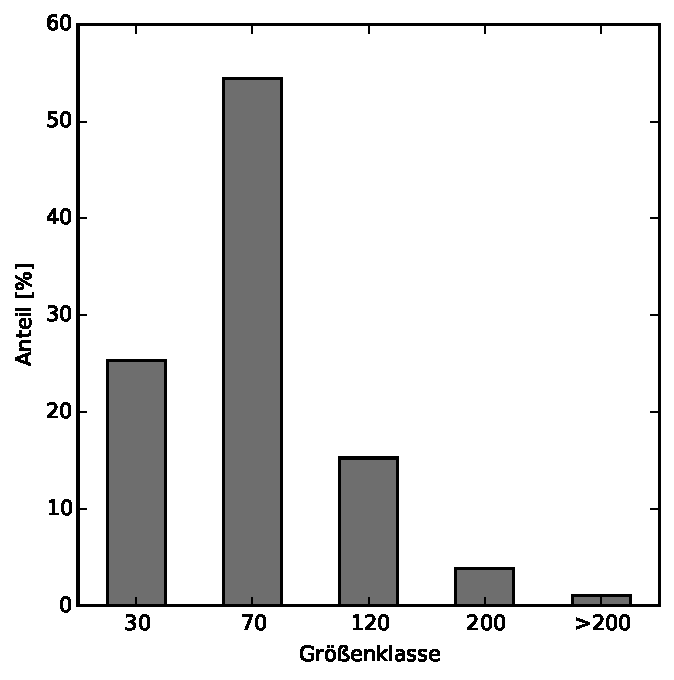
\includegraphics[height=.9\textwidth]{fig/2-2-1_KeramikFragmentierung.pdf}
\caption{Fragmentierung der Scherben (Größenklassen siehe Anm.~\ref{ftn:Keramik_Fragmentierung}).\newline}
\label{KeramikFragmentierung}
\end{subfigure}\hfill
\begin{subfigure}{\columnwidth}
\centering
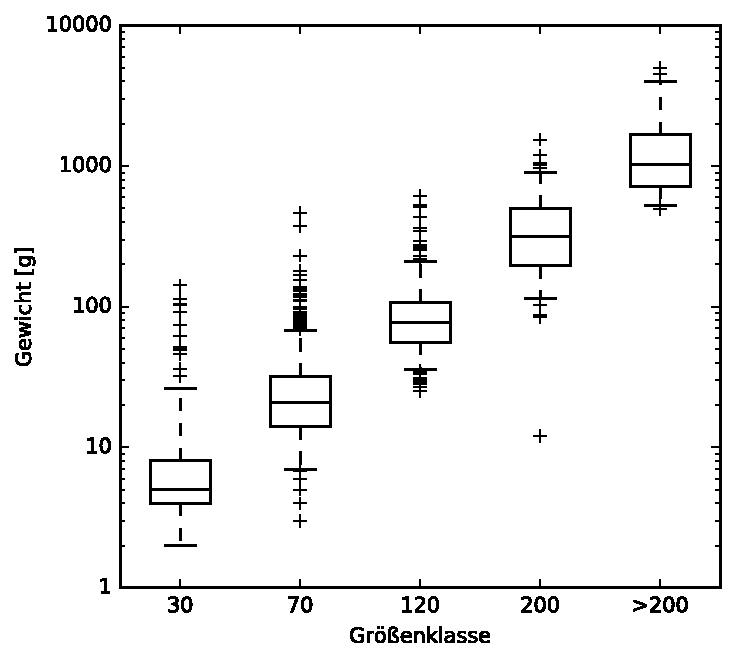
\includegraphics[height=.9\textwidth]{fig/2-2_Keramik_Gr-Gew_BoxPlt_2.pdf}
\caption{Verhältnis von Scherbengröße und Gewicht (Größenklassen siehe Anm.~\ref{ftn:Keramik_Fragmentierung}; 4218~GE).}
\label{fig:Keramik_FragmGrGew_B}
\end{subfigure}
\caption{Funde: Fragmentierung.}
\label{fig:Keramik_Typen-Fragm}
\end{figure*}

Der Anteil an unverzierten Stücken im Vergleich zu jenen GE aus dem untersuchten Materialkomplex, die Verzierungen aufweisen, variiert zwischen den Komplexen aus Oberflächensurveys und jenen aus Grabungen nur leicht. Während unverzierte Stücke in Oberflächenabsammlungen etwa 25\,\% ausmachen, sind es bei den ausgegrabenen Komplexen (Kat.-Nr.~1--19) knapp 29\,\%. Im Anschluss an die Ausgrabung der beiden Komplexe PIK~87/1 (Kat.-Nr.~8) sowie PIK~87/2 (Kat.-Nr.~9) in Pikunda am \mbox{Sangha} (Fpl.~255) wurde nachweislich unverziertes Scherbenmaterial verworfen. Im vorliegenden und ausgewerteten Fundmaterial dieser beiden Grabungen machen unverzierte Stücke immer noch 26\,\% aller GE aus. Daraus kann gefolgert werden, dass die Selektion der Stücke im Gelände die Repräsentanz des Fundinventares nur teilweise beeinträchtigt hat. Die Grabungen in Maluba am Lua (Fpl.~230; Kat.-Nr.~1--5), für die ein Aussondern \textit{nicht-diagnostischer} Stücke nicht überliefert ist, umfassten hingegen lediglich 18\,\% unverzierte Scherben. Diese Angaben legen nahe, dass die Oberflächenabsammlungen, zumindest mit Blick auf das Verhältnis von verzierten zu unverzierten Stücken, nicht grundsätzlich unrepräsentativ sind.


\subsubsection{Erhaltung}

Von den insgesamt 4217 aufgenommenen Gefäßeinheiten bestehen nur 654 aus mehr als einer Scherbe. Im Mittel bestehen die Gefäßeinheiten aus etwa 1,5 Scherben, was eine sehr starke Fragmentierung anzeigt und als Indikator für eine schlechte Erhaltung gewertet werden kann \parencite[siehe][86]{Jesse.2003}. Das mittlere Gewicht einer Gefäßeinheit liegt bei knapp 67\,g, das mittlere Gewicht der Einzelscherben bei rund 51\,g.\footnote{Der Unterschied ist wohl einzig auf die stark schiefen Verteilungen zurückzuführen.} Die Fragmentierurng der GE beziehungsweise der Zerscherbtheitsgrad der Keramik wurde unter Nutzung einer Größenklassen-Systematik aufgenommen, welche zuletzt auch bei \textcite[89]{Clist.20042005} zur Anwendung kam.\footnote{Die im Rahmen der Aufnahme genutzten Größenklassen beschreiben die Fragmentierung der Stücke mittels fünf fester Klassen (siehe \textsc{Clist}~2004/2005:~89): \textit{stark fragmentierte} beziehungsweise \textit{kleine Stücken} sind jeweils kleiner als 30\,$\times$\,30\,mm. Im ursprünglich auf \textcite[379]{Joukowsky.1980} zurückgehenden Schema liegt die kleinste Klassengrenze bei 25\,$\times$\,25\,mm \parencites[nach][]{Claes.1985}{deMaret.1985}[89]{Clist.20042005}. \textit{Mittelgroße} beziehungsweise \textit{mittelstark fragmentierte Stücke} sind zwischen  30\,$\times$\,30\,mm und 70\,$\times$\,70\,mm groß. Die nächste Klassengrenze liegt bei 120\,$\times$\,120\,mm und beschreibt \textit{gering fragmentierte} beziehungsweise \textit{große Stücke}. Stücke mit einer Größe zwischen 120\,$\times$\,120\,mm und 200\,$\times$\,200\,mm sind \textit{kaum fragmentiert} beziehungsweise \textit{groß}, während Objekte größer als 200\,$\times$\,200\,mm in der Regel große Gefäßfragmente oder ganze Gefäße widerspiegeln. Eine Dokumentation der erhalten Anteile von Gefäßprofilen und Randdurchmessern erfolgte nicht \parencite[siehe hierzu][155\,f.]{Claen.2011}. Die genannten Größenklassen wurden auch auf das nichtkeramische Fundgut, etwa Schlacken angewandt.\label{ftn:Keramik_Fragmentierung}} Während etwa 25\,\% der Keramik sehr stark fragmentiert sind -- kleiner als 30\,$\times$\,30\,mm -- sind knapp über die Hälfte der Scherben zwischen 30\,$\times$\,30\,mm und 70\,$\times$\,70\,mm groß (Abb.~\ref{KeramikFragmentierung}). Stücke größer als 70\,$\times$\,70\,mm sind seltener vertreten und machen zusammen nur etwa 20\,\% des Materials aus.


\begin{table*}[tb]
	\noindent\begin{minipage}[b]{\columnwidth}
		\centering
		{\footnotesize
			\begin{sftabular}{@{}llr@{}}
				\toprule
				\textbf{Schlüssel} & \textbf{Größenklasse} & \textbf{Durchmesser} \\
				\midrule
				VF & Very Fine & 62--125~$\mu$m \\
				F & Fine & 125--250~$\mu$m \\
				M & Medium & 250--500~$\mu$m \\
				C & Coarse & 500--1000~$\mu$m \\
				VC & Very Coarse & 1000--2000~$\mu$m \\
				\bottomrule
		\end{sftabular}}\vspace{1em}
		\captionof{table}{Keramik: Korngrößen nach der \textit{Wentworth-Grainsize-Scale}.\label{tab:Keramik_PartikelGr}}
	\end{minipage}\hfill
	\noindent\begin{minipage}[b]{\columnwidth}
		\centering
		{\footnotesize
			\begin{sftabular}{@{}lll@{}}
				\toprule
				\textbf{Schlüssel} & \textbf{Farbe} & \textbf{MUNSELL-Wert} \\
				\midrule
				S & schwarz/black & 10 YR 2/1 \\
				G & grau/grey & 10 YR 6/1 \\
				W & weiß/white & 10 YR 8/1 \\
				Bg & beige-ocker/yellow & 10 YR 8/6 \\
				Br & braun/dark reddish brown & 2.5 YR 3/4 \\
				R & rot/red & 2.5 YR 4/8--5/8 \\
				\bottomrule
		\end{sftabular}}
		\captionof{table}{Keramik: Farben der Scherbenoberflächen und -brüche.\label{tab:Keramik_Farbe}}
	\end{minipage}
\end{table*}

Die fünf Größenklassen bilden die Fragmentierung in einem zufriedenstellenden Maß ab, wie eine Gegenüberstellung mit den individuellen Scherbengewichten ergab (Abb.~\ref{fig:Keramik_FragmGrGew_B}). Trotz Ausreißern zeigen die Verteilungen, dass für jede der Größenklassen ein Gewichtsbereich angegeben werden kann, welcher sich von jenem einer anderen Größenklasse im Interquartilabstand unterscheidet. Überlappungen der Verteilungen stellen sich erst bei Betrachtung der zweifachen Standardabweichung ein.\footnote{Zur Interpretation von Box-Whisker-Plots siehe auch \textcite[81]{Hedderich.2016}. Im Fall von Abb.~\ref{fig:Keramik_FragmGrGew_B} markieren die Whiskers beziehungsweise Antennen die 2-Sigma-Standardabweichung der jeweiligen Verteilungen, während die Box das untere (25\,\%) sowie das obere Quartil (75\,\%) anzeigt und die zentrale Linie den Median markiert. Wird die einfache Standardabweichung zugrunde gelegt, lässt sich keine Überschneidung der Verteilungen beobachten.} Die Verteilungen zeigen insgesamt eine breite Streuung mit einigen Ausreißern, überlagern sich aber nur im Randbereich.


\subsubsection{Technologie}\label{sec:AufnahmeTechnologie}

Zusätzlich zu einer formalen Analyse, die sich auf morphologische Charakteristika wie Verzierung der Keramik stützt (siehe Kap.~\ref{sec:Keramiksequenz}), bildet eine tiefgreifende Auseinandersetzung mit technischen Parametern eines der Kernziele der Untersuchung. Hierfür grundlegend war die Einbeziehung von keramik-technischen Parametern in das Aufnahmesystem. Die untersuchten Kriterien gründen vornehmlich auf den Untersuchungen von \textcite{Nordstrom.1972} zu sudanesischer Keramik, welche wiederum Ausgangspunkt der neuen Studie von \textcite{Riemer.2011} zu Material aus der Dakhla-Oase in Ägypten waren, an der sich die hier vorgelegte Untersuchung orientiert. Für die Analyse der technologischen Eigenschaften der Gefäßkeramik wurde ein Katalog aus Aufnahmekriterien formuliert, welcher die folgenden Kenngrößen umfasst:
\begin{itemize*}
	\item nichtplastische Partikel
	\begin{itemize*}
		\item Größe (nach \textit{Wentworth-Grainsize-Scale})
		\item Dichte \parencites[32]{Kinne.2009}[nach][]{Hodgson.1976}
		\item Art
	\end{itemize*}
	\item Farbe des Scherben
	\begin{itemize*}
		\item Kernfarbe
		\item (Brennfarbe)
		\item Unterteilung des Scherbens in Oxidationszonen
		\item Ausbildung der Grenze zwischen Oxidationszonen
	\end{itemize*}
	\item Strukturierung der Oberfläche
\end{itemize*}

\begin{figure*}[!tb]
	\centering
	\resizebox{\textwidth}{!}{%
		{\footnotesize
\begin{sftabular}{@{}m{.02\textwidth} m{.02\textwidth} *7{>{\centering\arraybackslash}m{.1\textwidth}} m{.25\textwidth} @{}m{0pt}@{}@{}} 
 &  & \multicolumn{7}{c}{\textit{Variante}} &  &  \\
 &  & \textbf{1} & \textbf{2} & \textbf{3} & \textbf{4} & \textbf{5} & \textbf{6} & \textbf{7} & & \\
\multirow{10}{*}{\rotatebox[origin=c]{90}{\textit{Grundform} \hspace{9cm}}} & \textbf{A} & 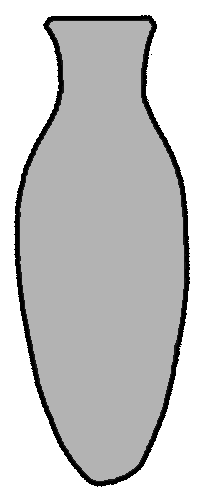
\includegraphics[height=.1\textwidth]{fig/Abb_GefFormen/G11c_Bolongo101.png} & 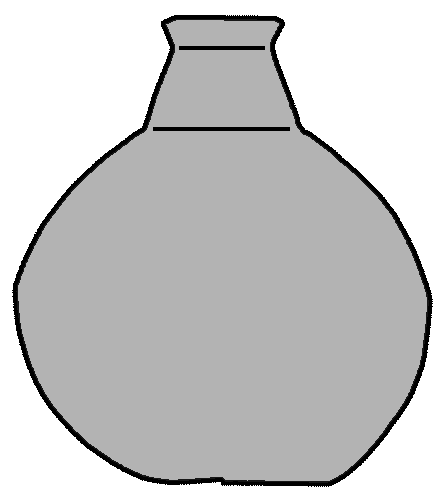
\includegraphics[height=.1\textwidth]{fig/Abb_GefFormen/G11b_MUN87-1-0-2-6-2.png} & 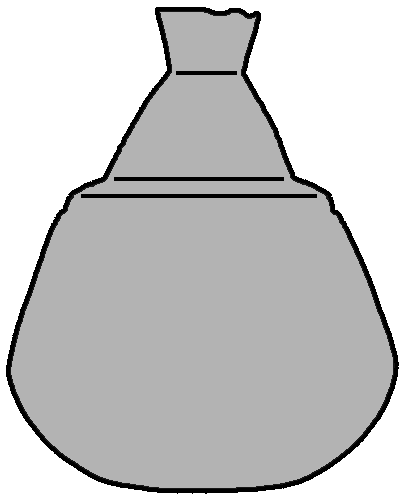
\includegraphics[height=.1\textwidth]{fig/Abb_GefFormen/G11a_MSG87-102-9a.png} &  &  &  &  & Flaschenförmige Gefäße & \\[.11\textwidth]
 & \textbf{B} & 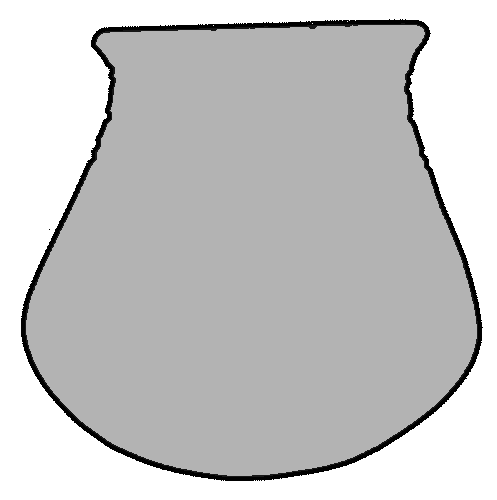
\includegraphics[height=.1\textwidth]{fig/Abb_GefFormen/G5_MUN87-2-1-3-8.png} & 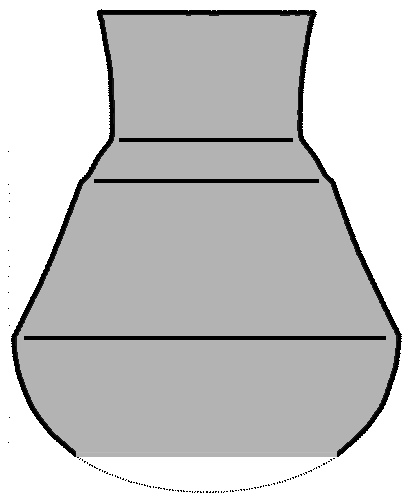
\includegraphics[height=.1\textwidth]{fig/Abb_GefFormen/G6c_msn87-101-145.png} & 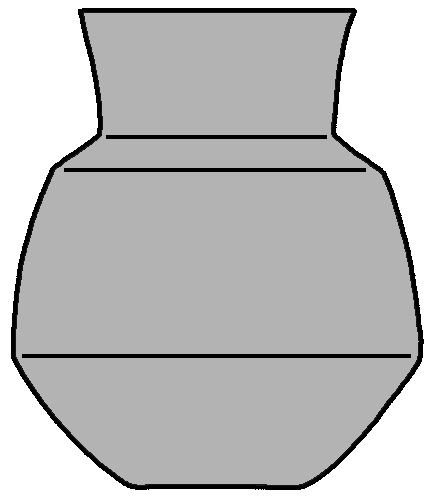
\includegraphics[height=.1\textwidth]{fig/Abb_GefFormen/G6b_ITN87-103-3a.png} & 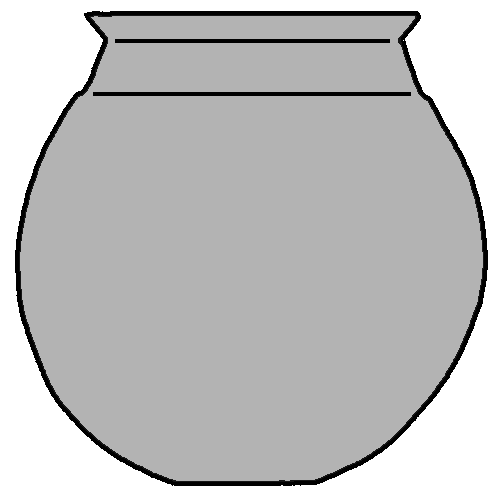
\includegraphics[height=.1\textwidth]{fig/Abb_GefFormen/G6a_MUN87-1-0-2-1.png} & 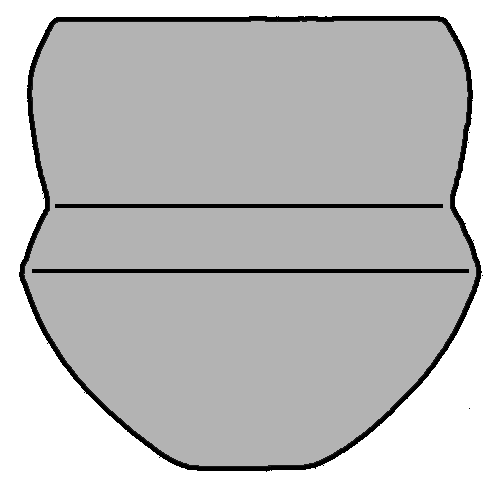
\includegraphics[height=.1\textwidth]{fig/Abb_GefFormen/G13_MKL85-101-114.png} & 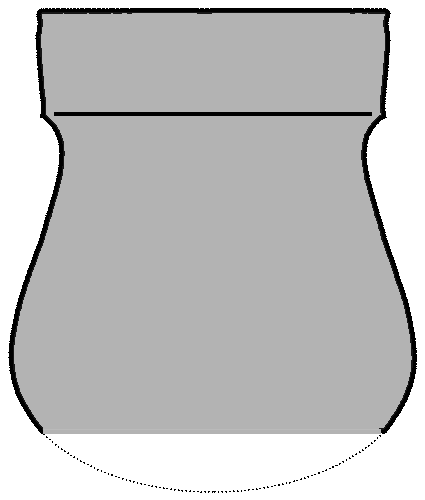
\includegraphics[height=.1\textwidth]{fig/Abb_GefFormen/G4_PIK87-101-51.png} & 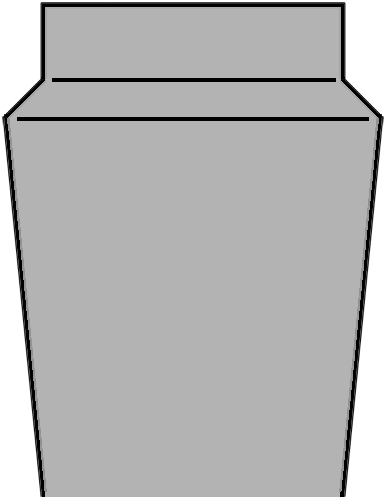
\includegraphics[height=.09\textwidth]{fig/Abb_GefFormen/G4b.png} & hohe Gefäße & \\[.11\textwidth]
 & \textbf{C} & 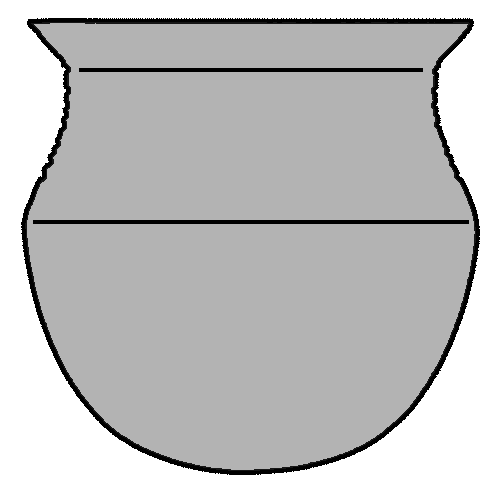
\includegraphics[height=.08\textwidth]{fig/Abb_GefFormen/G7a_NGB85-101-131.png} & 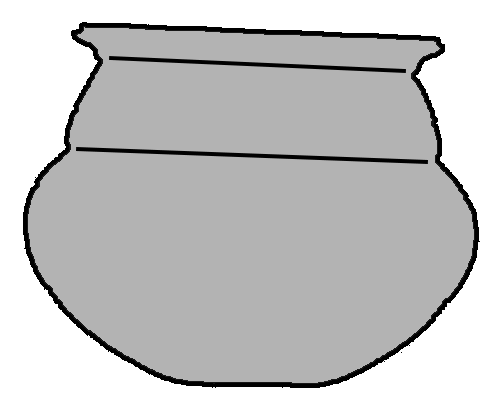
\includegraphics[width=.1\textwidth]{fig/Abb_GefFormen/G7b_DON85-102-a.png} &  &  &  &  &  & Gefäße mit leicht konvexer Wandung und ausgeprägtem Halsbereich & \\[.11\textwidth]
 & \textbf{D} & 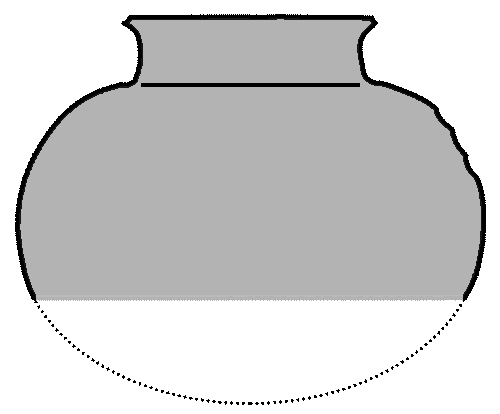
\includegraphics[width=.1\textwidth]{fig/Abb_GefFormen/G7c_PIK87-1-2-3_1-3-7.png} & 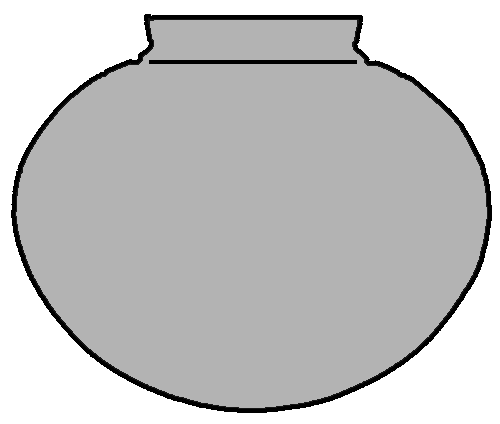
\includegraphics[width=.1\textwidth]{fig/Abb_GefFormen/G10a_NGO87-102-28-29.png} &  &  &  &  &  & Gefäße mit stark konvexer Wandung ohne ausgeprägten Halsbereich & \\[.11\textwidth]
 & \textbf{E} & 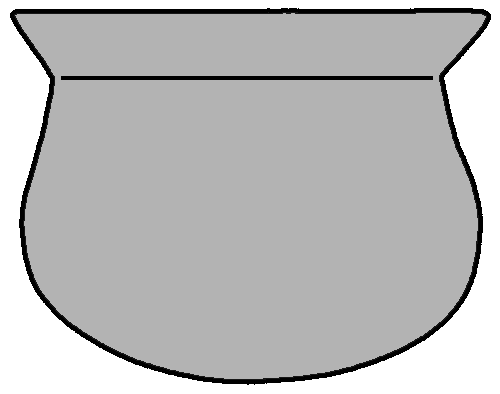
\includegraphics[width=.1\textwidth]{fig/Abb_GefFormen/G3_BLK87-1-1-1-2_HS.png} & 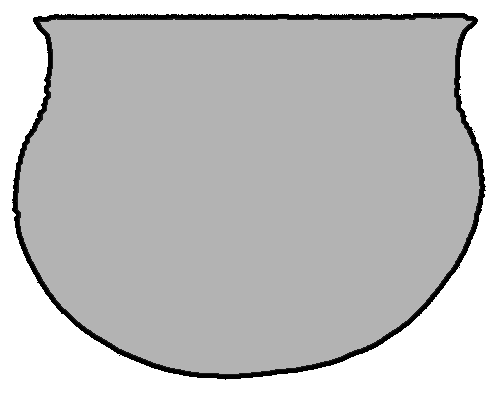
\includegraphics[width=.1\textwidth]{fig/Abb_GefFormen/G3c_MBN85-501-2.png} & 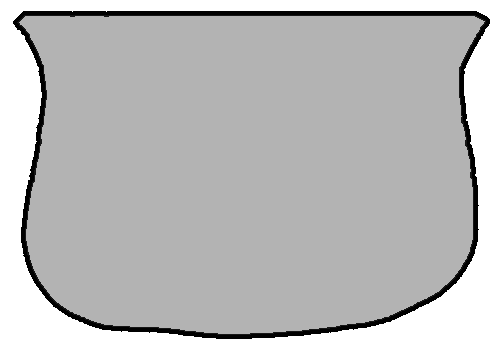
\includegraphics[width=.1\textwidth]{fig/Abb_GefFormen/G1b_MUN87-2-1-3.png} & 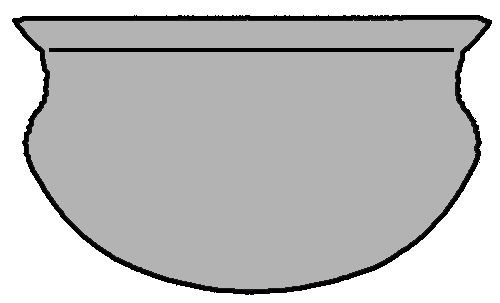
\includegraphics[width=.1\textwidth]{fig/Abb_GefFormen/G8b1_BLN85-201-b.png} & 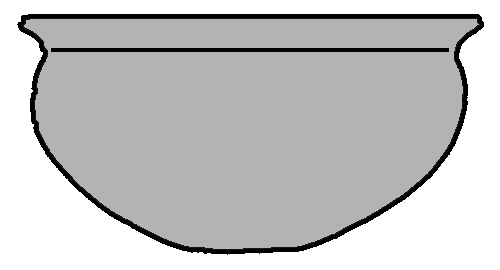
\includegraphics[width=.1\textwidth]{fig/Abb_GefFormen/G9b_DON85-102-b.png} & 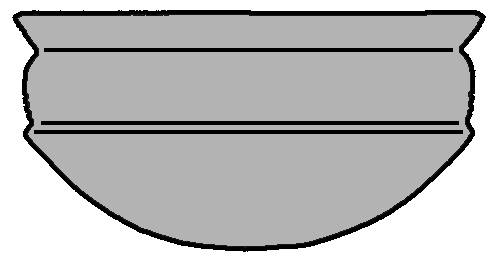
\includegraphics[width=.1\textwidth]{fig/Abb_GefFormen/G2d_SSL87-101-142.png} & 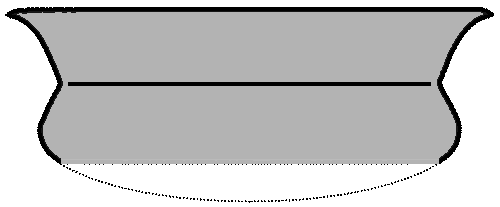
\includegraphics[width=.1\textwidth]{fig/Abb_GefFormen/G3b_GE5_BLK87-1-1-3-1-3.png} & Gefäße mit geschweifter Wandung & \\[.11\textwidth]
 & \textbf{F} & 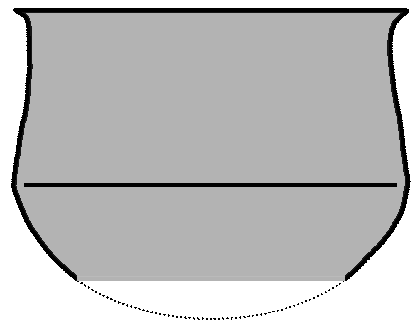
\includegraphics[width=.1\textwidth]{fig/Abb_GefFormen/G1c_LKW87-401-1.png} & 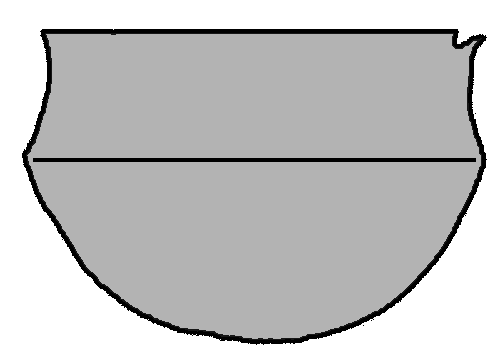
\includegraphics[width=.1\textwidth]{fig/Abb_GefFormen/G1d_MBJ_Roulettekeramik_E87-010-25.png} & 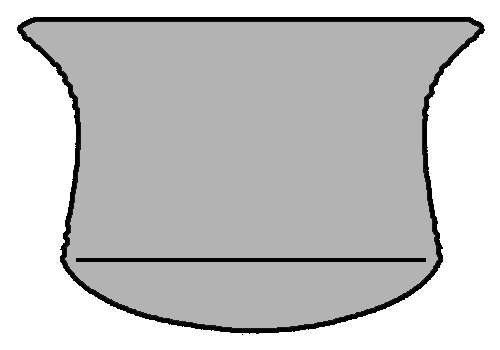
\includegraphics[width=.1\textwidth]{fig/Abb_GefFormen/G1a_PIK87-101-58.png} & 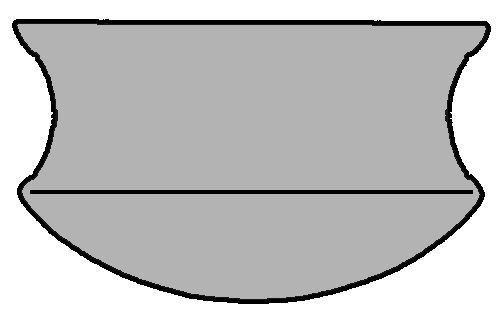
\includegraphics[width=.1\textwidth]{fig/Abb_GefFormen/G1a2_NGO87-102-27.png} & 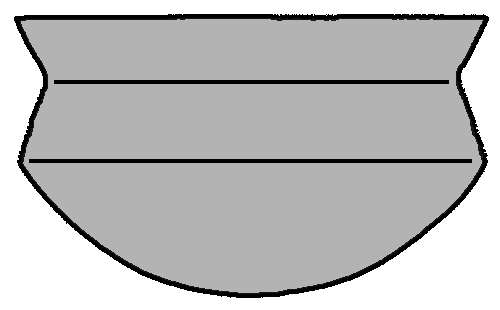
\includegraphics[width=.1\textwidth]{fig/Abb_GefFormen/G2e_INS87-102-2.png} & 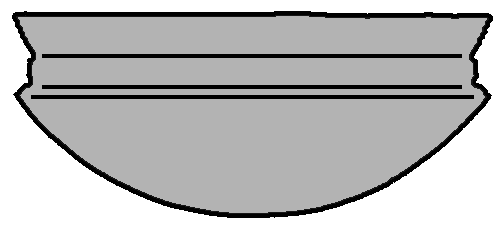
\includegraphics[width=.1\textwidth]{fig/Abb_GefFormen/G2a_NGO87-102-21.png} & 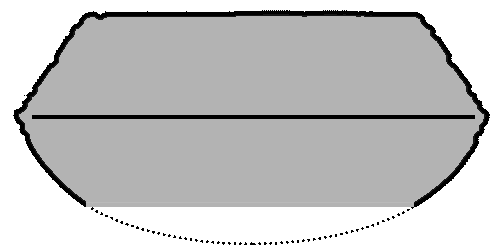
\includegraphics[width=.1\textwidth]{fig/Abb_GefFormen/G2h_MND85-101-33etc.png} & Gefäße mit abknickender Wandung & \\[.11\textwidth]
 & \textbf{G} & 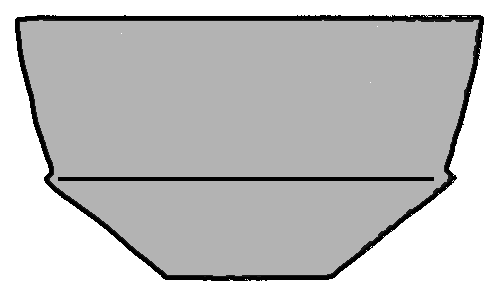
\includegraphics[width=.1\textwidth]{fig/Abb_GefFormen/G2b_ITN87-103-9.png} & 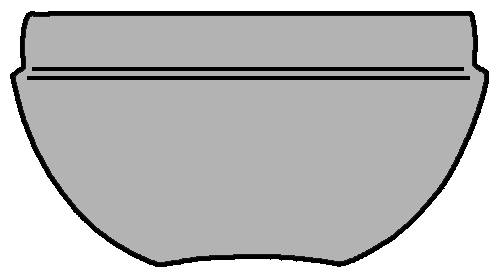
\includegraphics[width=.1\textwidth]{fig/Abb_GefFormen/G2c_MSG87-102-11.png} & 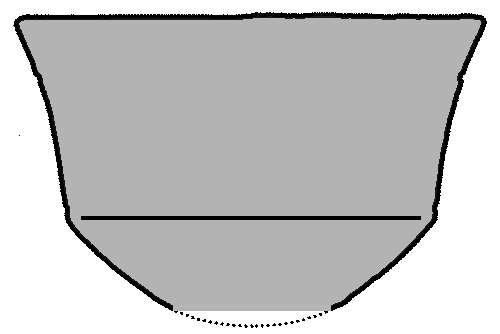
\includegraphics[width=.1\textwidth]{fig/Abb_GefFormen/G2f_MSG87-101-49.png} & 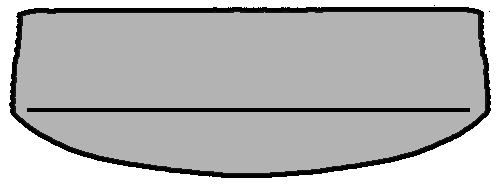
\includegraphics[width=.1\textwidth]{fig/Abb_GefFormen/G2g_GE2_BLK87-1-1-3-1-2.png} & 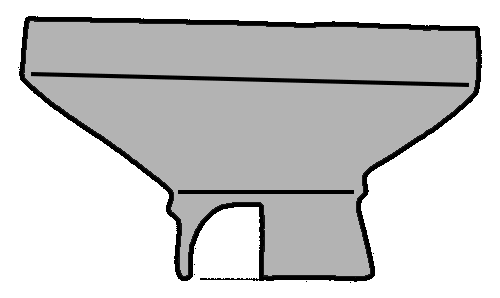
\includegraphics[width=.1\textwidth]{fig/Abb_GefFormen/G2g_MUN87-1-0-2-3-1.png} & 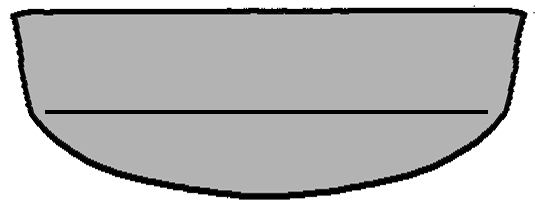
\includegraphics[width=.1\textwidth]{fig/Abb_GefFormen/G8c_Coart1907_TafXII175_neu.png} &  & Schalenförmige Gefäße mit abknickender Wandung & \\[.11\textwidth]
 & \textbf{H} & 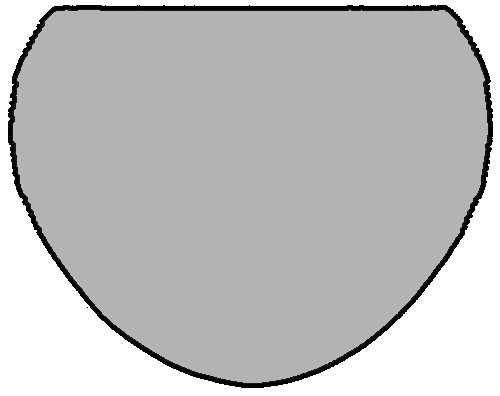
\includegraphics[width=.1\textwidth]{fig/Abb_GefFormen/G8e_kpt85-101-10.png} & 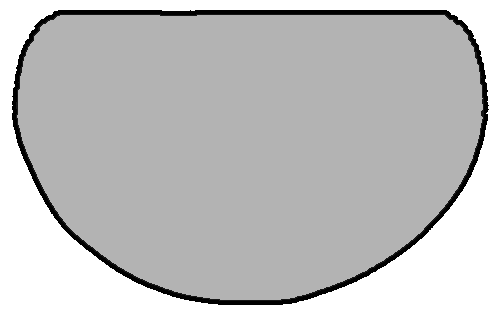
\includegraphics[width=.1\textwidth]{fig/Abb_GefFormen/G8d_MBN85-501-1.png} &  &  &  &  &  & Schalenförmige Gefäße mit konvexer Wandung und einbiegendem Rand & \\[.11\textwidth]
 & \textbf{I} & 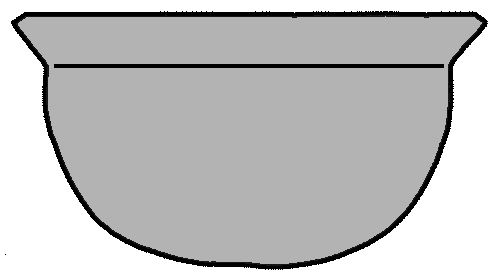
\includegraphics[width=.1\textwidth]{fig/Abb_GefFormen/G8b_BYN87-101-9.png} & 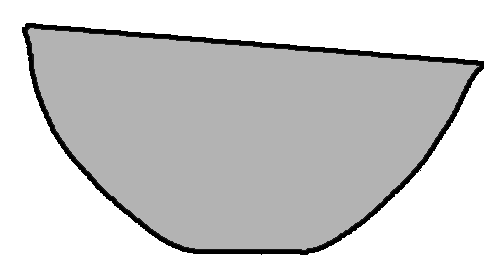
\includegraphics[width=.1\textwidth]{fig/Abb_GefFormen/G9a_DON85-102-120.png} & 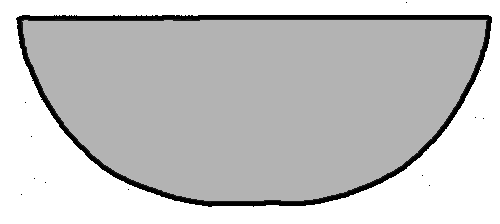
\includegraphics[width=.1\textwidth]{fig/Abb_GefFormen/G8a_BTW87-101-43.png} & 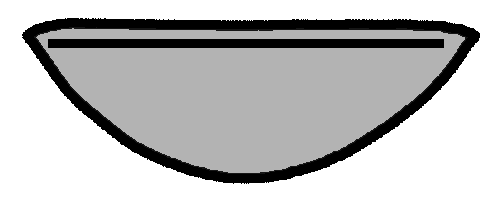
\includegraphics[width=.05\textwidth]{fig/Abb_GefFormen/G8a2_ngk01_PDM87-101-105.png} &  &  &  & Schalenförmige Gefäße mit konvexer Wandung & \\[.11\textwidth]
 & \textbf{J} & 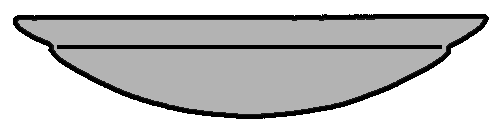
\includegraphics[width=.1\textwidth]{fig/Abb_GefFormen/G12a_NGO87-102-30.png} &  &  &  &  &  &  & Tellerförmige Gefäße & \\[.11\textwidth]
%\bottomrule
\end{sftabular}
}}
	\caption{Keramik: Gefäßtypen (G6 nach \cite[Taf.~XII.175]{Coart.1907}).}
	\label{tab:Keramik_GefFormen}
\end{figure*}

\noindent Von zentraler Bedeutung sind die Eigenschaften der im Scherben enthaltenen nichtplastischen Partikel. Diese wurden entsprechend ihrer Größe und Art sowie dem Anteil, in dem sie vorkommen, aufgenommen. Die Größe der Partikel wurden entsprechend der international anerkannten \textit{Wentworth-Grainsize-Scale} \parencite[381 Tab.~1, 388 Abb.~3]{Wentworth.1922} aufgenommen, wobei fünf Größenklassen unterschieden wurden (Tab.~\ref{tab:Keramik_PartikelGr}).\footnote{Die Bestimmung der Größenklassen erfolgte makroskopisch sowie unter Zuhilfenahme einer 10-fach vergrößernden Lupe in Referenz zu einer Korngrößen-Karte der Firma \textit{Precision Core} (Denver).} Die Verrundung und Sortierung der Partikel wurden nicht systematisch aufgenommen. Der Anteil an nichtplastischen Partikeln im Scherben wurde auf Basis einer Vergleichstafel zum Abschätzen von Anteilsklassen ermittelt \parencites[32]{Kinne.2009}[nach][]{Hodgson.1976}. Die Ansprache der Art der Partikel erfolgte basierend auf makroskopisch sichtbaren Kriterien und den Erfahrungen des Autors.

Zusätzlich zu diesen Eigenschaften der im Scherben beobachtbaren nichtplastischen Partikel erfolgte eine systematische Aufnahme der farblichen Zonierung der Stücke. Die farblichen Abstufungen der Keramik wurden mittels einer fünf Zonen umfassenden Unterteilung der Stücke sowie sechs Farbklassen\footnote{Zur Frage der Nutzung von Farbklassen entgegen der Aufnahme individueller MUNSELL-Farbwerte sei an dieser Stelle exemplarisch auf die Diskussion durch \textcite[38]{Keding.1997} verwiesen.} umfassenden Systematik erfasst (Tab.~\ref{tab:Keramik_Farbe}). Die fünf unterschiedenen Zonen gliedern sich in die äußere und innere Oberfläche des Stücks sowie drei Zonen im Profil beziehungsweise Bruch: den Bereich nahe der Außen- sowie Innenseite sowie der Kernbereich selbst. Die Oberflächenfarbe wurde als \textit{basic surface colour} nach \textcite[44\,f.]{Nordstrom.1972} aufgenommen. Die Ausbildung der Grenze zwischen den farblichen Zonen im Profil wurde in Anlehnung an \textcite[27]{Kinne.2009} umschreibend erfasst.

\begin{figure*}[p]
	\noindent\begin{minipage}[b]{\columnwidth}
		\centering
		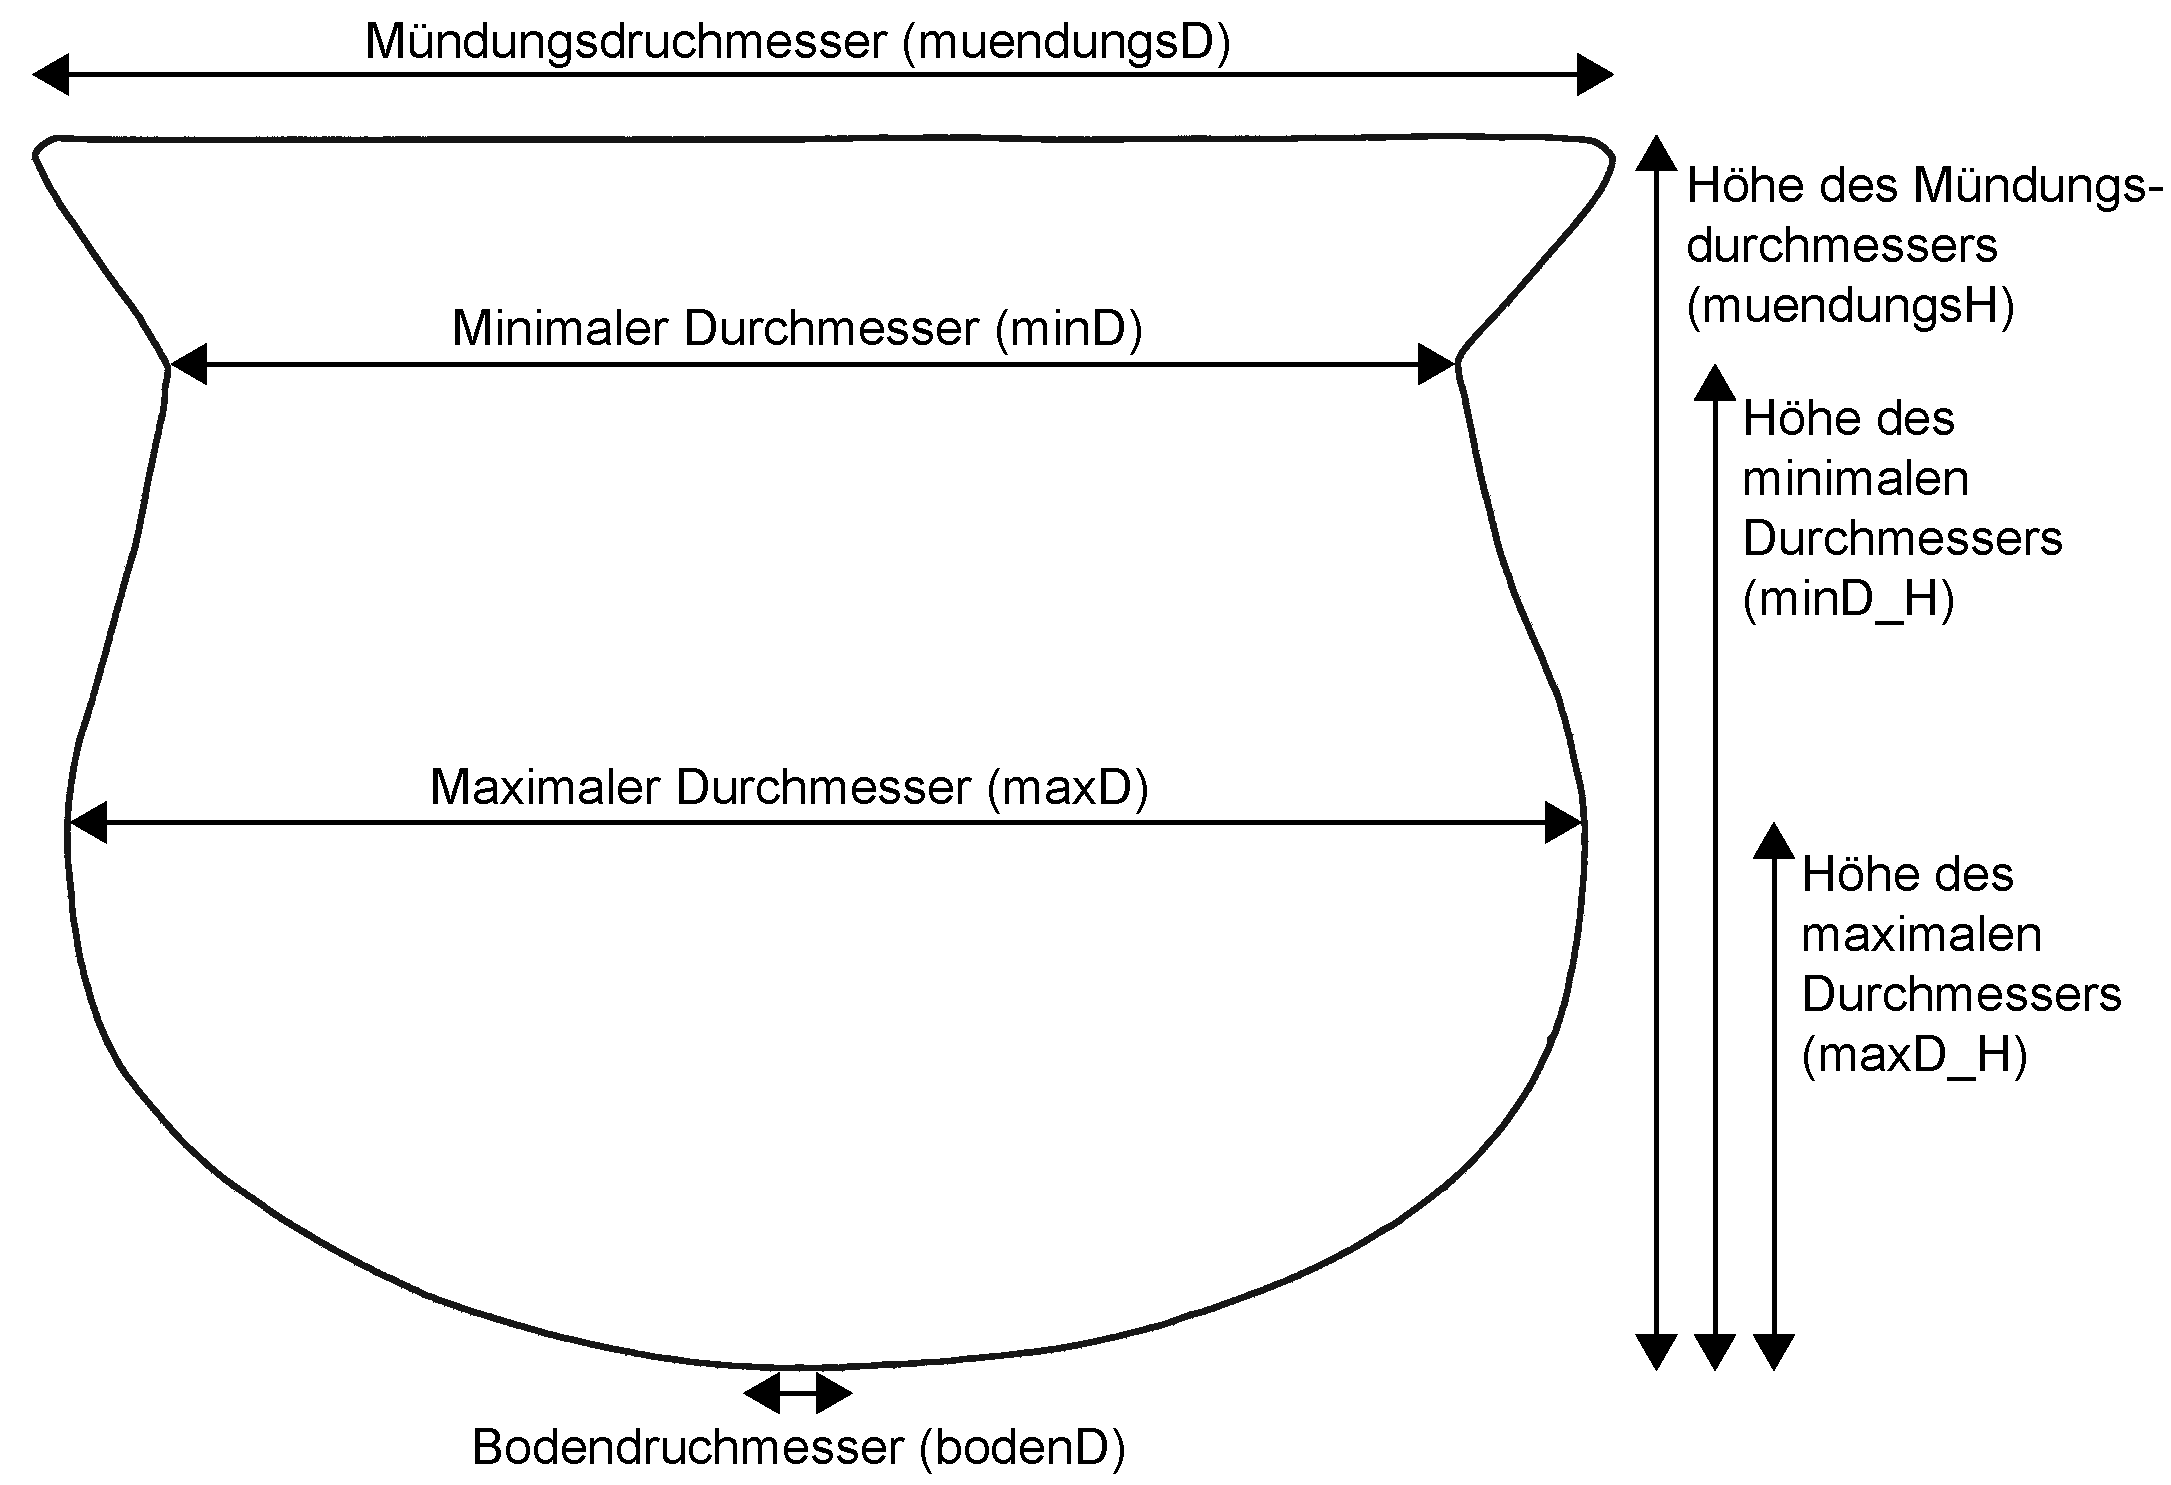
\includegraphics[width=\textwidth]{fig/GefaesseAbmessungenSystematik.pdf}
		\captionof{figure}{Keramik: Aufnahmeschema für die Gefäßabmessungen \parencite[nach][]{Wicke.2011}.\label{fig:GefAbmessungen_Schema}\\}
		\vspace{4cm}\captionof{figure}{Keramik: Systematik der Gefäßzonen, die für die Beschreibung morphologischer Ausprägungen sowie Verzierungen herangezogen wurde.\label{fig:Keramik_VerzZonen}}
	\end{minipage}\hfill
	\noindent\begin{minipage}[b]{\columnwidth}
		\centering
		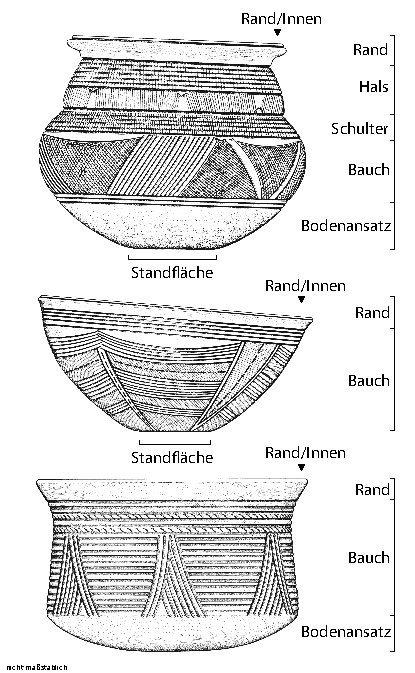
\includegraphics[width=\textwidth]{fig/Keramik_Systematik_Verzierungszonen.pdf}
	\end{minipage}
\end{figure*}

Die Oberflächenstruktur der Stücke wurde unter Referenz auf eine grobe, subjektive Ansprache als \textit{glatt}, \textit{leicht rau} oder \textit{rau} erfasst. Die bei der Keramik der Mandombe-Gruppe (Kap.~\ref{sec:MDB-Gr}) beobachtete Schlicker-Rauung der Gefäßunterteile (siehe Taf.~47.24) wurde als entsprechende Eigenschaft der Oberfläche erfasst. Spezifische Behandlungen der Oberfläche, wie Engoben, wurden hingegen gesondert, gemeinsam mit Anhaftungen an den Stücken aufgenommen. Für diese Oberflächenbehandlungen wurde keine Systematik herangezogen, die Beobachtungen wurden beschreibend in der Datenbank verzeichnet.

Die sich aus diesen technischen Eigenschaften des Scherbens ergebenden Gruppen wurden als \textit{Fabrics} konzeptualisiert und werden in Kap.~\ref{sec:Herstellung2_Fabric} detailliert besprochen.

%\pagebreak
\subsubsection{Form}

\paragraph{Gefäßform}\hspace{-.5em}|\hspace{.5em}%
Im Rahmen der Auswertung der Gefäßkeramik konnten zehn verschiedene Grundformen unterschieden werden (Abb.~\ref{tab:Keramik_GefFormen} A--J). Diese ließen sich weiter in Varianten (Abb.~\ref{tab:Keramik_GefFormen} 1--7) differenzieren, wodurch sich 41 Gefäßtypen ableiten ließen. Die gewählte Systematisierung der beobachteten Formen war für die angestrebte diachrone Untersuchung unerlässlich, da sich Gefäßformen einerseits zwar im Zeit-Raum-Kontinuum verändern, andererseits sich die Grundformen aber auch immer wiederholen \parencite[86]{Saev.2015}. Die von \textcite[39\, f.]{Wotzka.1995} genutzte Systematisierung, die nur grobe Grundformen wie Topf, Schale, Teller oder Flasche kennt und zusammengenommen 115 Gefäßtypen umfasst, konnte aufgrund ihrer spezifisch auf das Material aus dem Inneren Kongobecken zugeschnittenen Ausprägung nicht übernommen werden.\columnbreak

Insgesamt war bei 2178 Gefäßeinheiten (41\,\%) eine Ansprache der Gefäßform möglich. Die Proportionen der GE wurden, wo das Abnehmen der entsprechenden Maße möglich war, unter Einsatz von sieben Messstrecken systematisch erfasst \parencite[Abb.~\ref{fig:GefAbmessungen_Schema}; siehe][]{Wicke.2011}.\footnote{Im Laufe der Materialaufnahme erwies es sich als problematisch, dass das verwendete Aufnahmeschema für die Höhenwerte von der Standfläche eines Gefäßes ausgeht. Bei einer hohen Zahl von GE fehlte der untere Gefäßteil. Die Höhen der Randabschlüsse und minimaler sowie maximaler Durchmesser ließen sich so nicht aufnehmen. Da das Problem erst spät in der Aufnahme zu Tage trat, wurde von einer systematischen Anpassung der Vermessung abgesehen. In Fällen, in denen eine Bestimmung der fehlenden Partie in akzeptabler Weise möglich schien, wurde die hypothetische Position der Standfläche rekonstruiert und protokolliert.} Die Abmessungen wurden mit einer Messgenauigkeit von 0,5\,cm aufgenommen, wodurch die Proportionen der von Hand aufgebauten Keramik des Arbeitsgebiets angemessen repräsentiert sind.\footnote{Der Unterschied zwischen Mündungsweite, der tatsächlichen Gefäßöffnung und dem Randdurchmesser wurde nicht ausdifferenziert \parencite[siehe][88]{Saev.2015}.}

Die morphologischen Ausprägungen einzelner GE, wie auch die Verzierung (siehe Kap.~\ref{sec:AufnahmeVerzierungen}), wurden mit Bezug auf vordefinierte Gefäßzonen aufgenommen (Abb.~\ref{fig:Keramik_VerzZonen}). Die Abgrenzung der einzelnen Zonen wurde auf Basis markanter Wendepunkte am Profilverlauf der GE vorgenommen.

\begin{figure*}[p]
	\noindent\begin{minipage}[b]{\columnwidth}
		\centering
		{\footnotesize
			\begin{sftabular}{@{} >{\centering\arraybackslash} m{.01\textwidth} >{\centering\arraybackslash} m{.19\textwidth} >{\centering\arraybackslash} m{.19\textwidth} >{\centering\arraybackslash} m{.19\textwidth} >{\centering\arraybackslash} m{.19\textwidth}@{}}
				%\toprule
				& \textbf{1} & \textbf{2} & \textbf{3} & \textbf{4} \\
				%\midrule
				\textbf{A} & 
\includegraphics[height=.2\textwidth]{fig/Abb_RandFormen/A1.pdf} & 
\includegraphics[height=.2\textwidth]{fig/Abb_RandFormen/A2.pdf} & \includegraphics[height=.2\textwidth]{fig/Abb_RandFormen/A3.pdf} & \includegraphics[height=.2\textwidth]{fig/Abb_RandFormen/A4.pdf} \\
				\textbf{B} & \includegraphics[height=.2\textwidth]{fig/Abb_RandFormen/B1.pdf} & \includegraphics[height=.2\textwidth]{fig/Abb_RandFormen/B2.pdf} & \includegraphics[height=.2\textwidth]{fig/Abb_RandFormen/B3.pdf} & \\
				\textbf{C} & \includegraphics[height=.2\textwidth]{fig/Abb_RandFormen/C1.pdf} & \includegraphics[height=.2\textwidth]{fig/Abb_RandFormen/C2.pdf} & \includegraphics[height=.2\textwidth]{fig/Abb_RandFormen/C3.pdf} & \\
				%\bottomrule
		\end{sftabular}}\vspace{2em}
		\captionof{figure}{Keramik: Unterschiedene Randformen. Grundformen A--B als Zeilen und Varianten in Spalten.\label{tab:Keramik_RandFormen}}
	\end{minipage}\hfill
	\noindent\begin{minipage}[b]{\columnwidth}
		\centering
		{\footnotesize
			\begin{sftabular}{@{}m{.1\textwidth}m{.1\textwidth}m{.69\textwidth}@{}}
				\toprule
				& \textbf{Typ} & \textbf{Beschreibung} \\
				\midrule
				\includegraphics[height=.1\textwidth]{tbl/Tab_MdgFormen/M1_ATANGANA1988OkoloS162_1.png} & M1 & rund \\
				\includegraphics[height=.1\textwidth]{tbl/Tab_MdgFormen/M2_ATANGANA1988OkoloS162_2.png} & M2 & spitz \\
				\includegraphics[height=.1\textwidth]{tbl/Tab_MdgFormen/M3_ATANGANA1988OkoloS162_3.png} & M3 & gerade/flach/horizontal abgestrichen \\
				\includegraphics[height=.1\textwidth]{tbl/Tab_MdgFormen/M4_ATANGANA1988OkoloS162_4.png} & M4 & gerillt \\
				\includegraphics[height=.1\textwidth]{tbl/Tab_MdgFormen/M5_schraegAussen.png} & M5 & schräg nach außen abgestrichen \\
				\includegraphics[height=.1\textwidth]{tbl/Tab_MdgFormen/M6_schraegInnen.png} & M6 & schräg nach innen abgestrichen \\
				\bottomrule
		\end{sftabular} }
		\captionof{table}{Keramik: Übersicht der Randlippe \parencite[erweitert nach][162\,f. Tab.~24]{Atangana.1988}.\label{tab:MdgFormen}}
	\end{minipage}
\end{figure*}

\begin{figure*}[!tb]
	\centering
	\includegraphics[width=.95\textwidth]{fig/Wotzka1995_440Taf6_modDS.jpg}
	\caption{Keramik: Bodenformen \parencite[nach][440 Taf.~6]{Wotzka.1995}.}
	\label{fig:Keramik_BodenFormen}
\end{figure*}

\paragraph{Randform}\hspace{-.5em}|\hspace{.5em}\label{sec:Randform}
Die Aufnahme der Ränder erfolgte gemäß einer Systematik, die sich in erster Linie an der grundsätzlichen Ausrichtung des Randes orientiert. Differenziert wurden parallele, ausbiegende sowie einbiegende Ränder (Abb.~\ref{tab:Keramik_RandFormen}: A--C). Innerhalb dieser Grundtypen wurden mehrere charakteristische Varianten unterschieden. Parallele Ränder können neben der einfachen Grundform auch als umgelenkte, T-förmige sowie verdickte Formen vorkommen (Abb.~\ref{tab:Keramik_RandFormen}: A2--A4). Aus- wie einbiegende Ränder wurden noch in konkave sowie konvexe Varianten unterschieden (Abb.~\ref{tab:Keramik_RandFormen}: B2--B3, C2--C3):

\vspace{1em}
\noindent\begin{tabular}{@{}ll@{}}
A1 & parallel \\
A2 & umgelegt \\
A3 & T-förmig \\
A4 & verdickt \\
B1 & ausbiegend \\
B2 & konkav ausbiegend \\
B3 & konvex ausbiegend \\
C1 & einbiegend \\
C2 & konkav einbiegend \\
C3 & konvex einbiegend \\
\end{tabular}
\vspace{1em}

\noindent An die Grundform angefügte Parameter \enquote{.1} sowie \enquote{.2} zeigen \textit{kurze} beziehungsweise \textit{lange} Varianten der entsprechenden Randform an. Spezifischere und diagnostische Variationen der Grundformen wurden im weiteren Verlauf der Aufnahme durch Hinzusetzen individueller Zählnummern, beginnend ab dem Schlüssel-Zusatz \enquote{.3}, angefügt. Insgesamt ergaben sich zehn Grundformen der Randgestaltung (Abb.~\ref{tab:Keramik_RandFormen}) sowie 26 unterscheidbare Variationen.\footnote{Wie bereits bei den Gefäßformen (Abb.~\ref{tab:Keramik_GefFormen}) spiegelt die gewählte Form der Systematisierung das Bestreben wider, die Aufnahme des Untersuchungsmaterials vor dem Hintergrund der dieser Arbeit zugrundeliegenden diachronen Fragestellungen durchzuführen.}

Die häufigste Randform, die einfach ausbiegenden Ränder (B1), macht 24,8\,\% aller bestimmten Randformen aus, gefolgt von konkav ausbiegenden Rändern (B2), die in 13,3\,\% aller Fälle beobachtet wurden. Die kurze Variante gerade ausbiegender Ränder (B1.1) macht 11,7\,\% aus, während parallel, gerade aufsteigende Ränder (A1) auf einen Anteil von 10\,\% kommen. Alle übrigen Varianten liegen jeweils im Bereich von unter 7\,\%. Zusammengenommen repräsentieren diese, einzeln nur selten vertretenen Formen, 40\,\% der aufgenommen Gefäßränder. Werden die unterschiedenen Variationen den jeweiligen Grundformen (Abb.~\ref{tab:Keramik_RandFormen}) zugerechnet, sind insgesamt 68,5\,\% aller Rändern ausbiegend (B), während 25\,\% parallel (A) verlaufen und nur 6,5\,\% einbiegend (C) sind.

\paragraph{Randlippe}\hspace{-.5em}|\hspace{.5em}%
Die Ausprägung der Randlippe, in diesem Zusammenhang auch \textit{Gefäßmündung} genannt, wurde in Anlehnung an die von \textcite[162f Tab.~24]{Atangana.1988} genutzte Systematik losgelöst von der Randform aufgenommen (Tab.~\ref{tab:MdgFormen}).\footnote{\textcite[48]{Wotzka.1995} erfasste die Ausprägung der Randlippe nicht separat, sie bildete vielmehr eine mögliche Variation des \textit{Randtyps} ab. Ähnlich ging auch \textcite[110]{Jesse.2003} vor.} Die Einteilung Atanganas wurde dabei um die beiden Formen M5 sowie M6, die schräg nach außen oder innen abgestrichene Randlippen widerspiegeln, erweitert. Die Varianten M1 bis M5 sind jeweils in Häufigkeiten zwischen 13,5 bis 26,4\,\% vertreten, schräg nach innen abgestrichene Randlippen des Typs M6 kommen mit nur 3,9\,\% deutlich seltener vor.

\paragraph{Bodenform}\hspace{-.5em}|\hspace{.5em}\label{sec:Bodenform}
Die Unterscheidung der Ausformung des Bodens gründete sich auf die von \textcite[440 Taf.~6]{Wotzka.1995} aufgestellten Systematik, die um eine Form B15 erweitert wurde. Die neue Bodenform B15 beschreibt Gefäße, die auf einzelnen \textit{Füßchen} stehen. Im untersuchten Material fanden sich lediglich zwei GE mit drei symmetrisch am Unterteil eines ansonsten rund ausgeformten Bodens angebrachten \textit{Füßchen} (Taf.~1.2, 2.1). Im Detail wurden folgende Bodenformen unterschieden (Abb.~\ref{fig:Keramik_BodenFormen}):
\setlength\LTleft{0pt}
\vspace{.25em}
\noindent\begin{tabular}{@{}ll@{}}
	B1 & Rundboden \\
	B2 & Linsenboden \\
	B3 & Spitzboden \\
	B4 & einfacher Flachboden \\
	B5 & innen aufgewölbter Flachboden  \\
	B6 & Flachboden mit konkaver Standfläche \\
	B7 & Omphalosboden \\
	B8 & Riefenprofilierter Flachboden \\
	B9 & Profiliert abgesetzter Flachboden \\
	B10 & Riefenabgesetzter Flachboden \\
	B11 & abgesetzter Flachboden \\
	B12 & Flachboden mit einziehender Unterseite\\
\end{tabular}
%\vspace{1em}

%\setlength\LTleft{0pt}
\vspace{.25em}
\noindent\begin{tabular}{@{}ll@{}}
	B13 & Standring / Hohlfuß \\
	B14 & massiver Standfussboden \\
	B15 & Boden mit abgesetzten Standfüßen \\
\end{tabular}
\vspace{1em}

\noindent Insgesamt konnte die Bodenform lediglich bei 6\,\% aller GE angesprochen werden. Dieser geringe Anteil liegt zu einen gewissen Grad an den Schwierigkeiten, die mit der Ansprache runder Böden (B1) verbunden sind, die leicht als Fragmente der Gefäßwandung fehlinterpretiert werden können. Zusammengenommen machen runde Böden (B1) knapp 49\,\% aller bestimmter Böden aus. Einfache Flachböden (B4) kommen mit 24\,\% am zweithäufigsten vor. Gefolgt werden sie von Linsenböden (B2) mit 6\,\%, Standringböden mit Hohlfuß (B13) mit ebenfalls 6\,\% sowie 5\,\% Flachböden mit konkaver Standfläche (B6). Die übrigen Formen kommen lediglich als Einzelfunde beziehungsweise bei weniger als zehn GE vor. Der von \textsc{Wotzka} (ebd. 440 Taf.~6) beschriebe Typ B14 wurde nicht beobachtet.

\subsubsection{Verzierung}\label{sec:AufnahmeVerzierungen}

Die Verzierungen der Keramik wurden für jede Gefäßeinheit individuell und in Referenz zur Gefäßregion aufgenommen (siehe Abb.~\ref{fig:Keramik_VerzZonen}).\footnote{Während formale Ansprachen wie die Gefäßform in einer 1:n-Beziehung in einer Datenbank abgebildet werden können (eine GE kann lediglich eine Gefäßform oder Randform aufweisen), können verschiedene Verzierungen auf verschiedenen Gefäßbereichen unterschiedlich häufig vorkommen. Die vorliegende Kardinalität der Entitätstypen \textit{Objekt}, \textit{Gefäßposition} und \textit{Verzierungselement} können in dem genutzten relativen Datenbankschema nicht direkt abgebildet werden. Die Entitäten jeder dieser Entitätstypen können mit beliebig vielen Entitäten der anderen beiden Entitätstypen in Beziehung stehen. Konkret ist hiermit gemeint, dass eine GE an verschiedenen Stellen auch mehrere Verzierungselemente aufweisen kann. Als Lösung wird eine Konkordanztabelle genutzt, welche die Primärschlüssel der genannten Entitätstypen als Fremdschlüssel-Paare beinhaltet. Die Beziehungen der drei Entitätstypen werden im Datenmodell durch drei getrennte 1:n-Beziehungen aufgelöst.} Basierend auf der Kombination aus Verzierungstechnik und -motiv wurden Verzierungselemente erarbeitet (Tab.~\ref{tab:Verzierungselemente}; Abb.~\ref{fig:Keramik_VerzSystematik}).\footnote{Die Klassifizierung der einzelnen Verzierungselemente lehnt sich dabei stark an \textsc{Wotzka} (1995) an, nimmt aber auch Aspekte aus Systematiken für die Bandkeramik \parencites{Stehli.1973}{Stehli.1977}{Kneipp.1998} und das südfranzösische Frühneolithikum auf \parencites[126\,f. Abb.~3]{Manen.2002}[auch bei][]{Linstadter.2013}. Die grafische Zusammenstellung der Klassifizierung in Abb.~\ref{fig:Keramik_VerzSystematik} folgt der Darstellungsweise von \textcite[80\,f. Abb.~39]{Keding.1997}.} Diese bilden in der Aufnahme der Verzierungen wie deren Auswertung die analytische Grundeinheit.

\begin{figure*}[p]
 \centering
 \includegraphics[width=.85\textwidth]{fig/VerzierungenSystematik.pdf}
 \caption{Keramik: Verzierungstechniken, Verzierungswerkzeuge und Verzierungselemente.}
 \label{fig:Keramik_VerzSystematik}
\end{figure*}

%\end{multicols}
%\afterpage{%
%\clearpage
\begin{table*}[p]

\begin{multicols}{2}
\noindent
{\scriptsize\begin{sftabular}{@{}m{.05\columnwidth} m{.1\textwidth} m{.63\columnwidth}@{}}
\toprule
\multicolumn{2}{@{}l@{}}{\textbf{Schlüssel}} &  \textbf{Kurzbeschreibung} \\
\midrule
01.1 & \includegraphics[width=.1\textwidth]{tbl/Tab_VerzElemente/V03a_PIK87-1-7-1.png} & \textit{Schachbrett}-Muster aus horizontalen und vertikalen Ritzlinien \\
01.2 & \includegraphics[width=.1\textwidth]{tbl/Tab_VerzElemente/V03b_PIK87-1-6-16.png} & \textit{Schachbrett}-Muster aus diagonalen Ritzlinien \\
01.3 & \includegraphics[width=.1\textwidth]{tbl/Tab_VerzElemente/V03c_PIK87-1-8-6.png} & \textit{Schachbrett}-Muster aus horizontalen und diagonalen Ritzlinien \\
01.4 & \includegraphics[width=.1\textwidth]{tbl/Tab_VerzElemente/V03d_PIK87-1-9-7.png} & \textit{Schachbrett}-Muster aus diagonalen und vertikalen Ritzlinien \\
01.5 & \includegraphics[width=.1\textwidth]{tbl/Tab_VerzElemente/V01b_PIK87-1-5-7.png} & Wellenlinien \\
01.6 & \includegraphics[width=.1\textwidth]{tbl/Tab_VerzElemente/V12a1_MSG87-102-8.png} & Zickzack-Linien \\
01.7 & \includegraphics[width=.1\textwidth]{tbl/Tab_VerzElemente/V12c_Gef9_CAM07-3-1-278-306.png} & Rillen in Fischgrät-Muster \\
01.8 & \includegraphics[width=.1\textwidth]{tbl/Tab_VerzElemente/V04d_PIK87-101-43-46.png} \includegraphics[width=.1\textwidth]{tbl/Tab_VerzElemente/V04e_NGO87-102-28-29.png} & Rillen gefüllte Flächen (Dreiecke, Rauten u.~a.) \\
01.9 & \includegraphics[width=.1\textwidth]{tbl/Tab_VerzElemente/V10a_PIK87-101-51.png} & feine vertikale oder horizontale Rillen \\
01.10 & \includegraphics[width=.1\textwidth]{tbl/Tab_VerzElemente/V10b_PIK87-101-40.png} & feine diagonale Rillen \\
01.11 & \includegraphics[width=.1\textwidth]{tbl/Tab_VerzElemente/V11b1_LKW87-186-1-2-5.png} & Muster aus überkreuzten Rillen \\
02.1 & \includegraphics[width=.1\textwidth]{tbl/Tab_VerzElemente/V01a_PIK87-1-8-6.png} & horizontale Riefen \parencite[siehe Muster \enquote{ISpeg5} von][251 Abb. 30.5 ]{GouemGouem.20102011} \\
02.2 & \includegraphics[width=.1\textwidth]{tbl/Tab_VerzElemente/V01c_PIK87-1-8-6.png} & vertikale Riefen \\
\bottomrule
\end{sftabular}}

\noindent
{\scriptsize\begin{sftabular}{@{}m{.05\columnwidth} m{.1\textwidth} m{.63\columnwidth}@{}}
\toprule
\multicolumn{2}{@{}l@{}}{\textbf{Schlüssel}} &  \textbf{Kurzbeschreibung} \\
\midrule
02.3 & \includegraphics[width=.1\textwidth]{tbl/Tab_VerzElemente/V01e_PIK87-1-8-6.png} & diagonale Riefen \\
02.4 & \includegraphics[width=.1\textwidth]{tbl/Tab_VerzElemente/V01e2_MLB85-1-3-2-5-35.png} & horizontales Band aus kurzen diagonalen Riefen \\
02.5 & \includegraphics[width=.1\textwidth]{tbl/Tab_VerzElemente/V01d_PIK87-101-7.png} & gebogene Riefen \\
02.6 & \includegraphics[width=.1\textwidth]{tbl/Tab_VerzElemente/V01f_MUN87-2-1-1-5-2.png} & spitz zusammenlaufende gebogene Riefen \\
02.7 & \includegraphics[width=.1\textwidth]{tbl/Tab_VerzElemente/V04c_PIK87-1-3-9.png} & sehr breite Riefen (\textgreater\,5\,mm) \\
03.1 & \includegraphics[width=.1\textwidth]{tbl/Tab_VerzElemente/V06e.png} & große Eindrücke, Fingereindrücke \\
04.1 & \includegraphics[width=.1\textwidth]{tbl/Tab_VerzElemente/V02a_PIK87-1-8-6.png} & Wiegeband mit Kamm \\
04.2 & \includegraphics[width=.1\textwidth]{tbl/Tab_VerzElemente/V02b_MUN87-2-1-1-4-2.png} & Wiegeband (siehe Muster \enquote{IIIPla1z} von \textsc{Gouem Gouem} 2010/2011: 117 Abb. 9.3.a ) \\
04.3 & \includegraphics[width=.1\textwidth]{tbl/Tab_VerzElemente/V05e_INS87-102-2.png} & gruppierte Eindrücke \\
04.4 & \includegraphics[width=.1\textwidth]{tbl/Tab_VerzElemente/V05f_SSL87-101-143.png} & gegenständige Eindrücke \\
04.5 & \includegraphics[width=.1\textwidth]{tbl/Tab_VerzElemente/V05j_SSL87-101-5.png} & kleine Flächen aus gegenständigen, halbrunden Eindrücken \\
04.6 & \includegraphics[width=.1\textwidth]{tbl/Tab_VerzElemente/V05h_DON85-102-a.png} & flache, winkelige Eindrücke \\
04.7 & \includegraphics[width=.1\textwidth]{tbl/Tab_VerzElemente/V05i1_MLB85-1-2-3.png} & kleine Kreisaugen-Eindrücke \\
& & \\[1mm]
\bottomrule
\end{sftabular}}
\end{multicols}
\caption{Keramik: Verzierungselemente. Für die ersten beiden Stellen der Schlüsselzahl -- die  Verzierungstechnik -- siehe \textsc{Wotzka} (1995: 44 Tab.~3).}
\label{tab:Verzierungselemente}
\end{table*}

\addtocounter{table}{-1}
\begin{table*}[p]
\begin{multicols}{2}
\noindent
{\scriptsize\begin{sftabular}{@{}m{.05\columnwidth} m{.1\textwidth} m{.63\columnwidth}@{}}
\toprule
\multicolumn{2}{@{}l@{}}{\textbf{Schlüssel}} &  \textbf{Kurzbeschreibung} \\
\midrule
04.8 & \includegraphics[width=.1\textwidth]{tbl/Tab_VerzElemente/V09l_MKA87-102-1.png} & dreieckige Eindrücke/Dreieckstempel \\
04.9 & \includegraphics[width=.1\textwidth]{tbl/Tab_VerzElemente/V09j_MIS87-101-56.png} & flächig angeordnete, horizontale Bänder kleiner Eindrücke \\
04.10 & \includegraphics[width=.1\textwidth]{tbl/Tab_VerzElemente/V09k_MIS87-101-56.png} & lose flächig verteilte kleine Eindrücke \\
04.11 & \includegraphics[width=.1\textwidth]{tbl/Tab_VerzElemente/V09i2_MKL85-101-114.png} & runde bis leicht ovale Eindrücke \\
04.12 & \includegraphics[width=.1\textwidth]{tbl/Tab_VerzElemente/V09a1_PIK87-1-14-1.png} & diagonale Eindrücke \\
04.13 & \includegraphics[width=.1\textwidth]{tbl/Tab_VerzElemente/V09n_SSL87-101-19.png} & leicht gewellte Bänder aus diagonalen oder vertikalen Eindrücken \\
04.14 & \includegraphics[width=.1\textwidth]{tbl/Tab_VerzElemente/V09a2_DON85-102-120.png} & horizontales oder vertikales Band aus linearen Eindrücken \\
04.15 & \includegraphics[width=.1\textwidth]{tbl/Tab_VerzElemente/V09b_PIK87-1-8-10.png} & vertikale Eindrücke \\
04.16 & \includegraphics[width=.1\textwidth]{tbl/Tab_VerzElemente/V09c1_PIK87-1-13-1.png} \includegraphics[width=.1\textwidth]{tbl/Tab_VerzElemente/V09c2_DON85-102-117.png} & Eindrücke in Rillen (siehe Muster \enquote{ISpeg5/ISpeg11} bei \textsc{Gouem Gouem} 2010/2011251, 251 Abb. 30.5) \\
04.17 & \includegraphics[width=.1\textwidth]{tbl/Tab_VerzElemente/V12b_INS87-102-2.png} & gegenständige Dreiecke in horizontalem Band \\
04.18 & \includegraphics[width=.1\textwidth]{tbl/Tab_VerzElemente/V11b2_DON85-102-126.png} & Bänder aus x-förmigen Eindrücken \\
04.19 & \includegraphics[width=.1\textwidth]{tbl/Tab_VerzElemente/V09h1_PDM87-101-12.png} & lange gebogene Eindrücke in Reihen \\
04.20 & \includegraphics[width=.1\textwidth]{tbl/Tab_VerzElemente/V09h2_MIT87-102-19.png} & kurze gebogene Eindrücke (Fingernagel) \\
04.21 & \includegraphics[width=.1\textwidth]{tbl/Tab_VerzElemente/V05i3_MBA11-1-1_DSC_0507_b.png} & Eindrücke mit Kaurischnecken oder Imitation \\
& & \\
\bottomrule
\end{sftabular}}

\noindent
{\scriptsize\begin{sftabular}{@{}m{.05\columnwidth} m{.1\textwidth} m{.63\columnwidth}@{}}
\toprule
\multicolumn{2}{@{}l@{}}{\textbf{Schlüssel}} &  \textbf{Kurzbeschreibung} \\
\midrule
05.1 & \includegraphics[width=.1\textwidth]{tbl/Tab_VerzElemente/V02c_PDM87-101-125.png} & diagonaler Kammeindruck \\
05.2 & \includegraphics[width=.1\textwidth]{tbl/Tab_VerzElemente/V12a3_MKL85-101-105.png} & Band aus zickzackartig angeordneten Kammeindrücken \\
05.3 & \includegraphics[width=.1\textwidth]{tbl/Tab_VerzElemente/V05a_PIK87-1-2-5.png} & Kammeindruck-Bänder \\
05.4 & \includegraphics[width=.1\textwidth]{tbl/Tab_VerzElemente/V05b_PIK87-101-8.png} & flächiger Kammeindruck \\
08 & \includegraphics[width=.1\textwidth]{tbl/Tab_VerzElemente/V07_MUN87-1-0-2-3-6.png} & \textit{Bnfwa-nfwa} \parencite[Muster: siehe][109--111]{Wotzka.1995} \\
09.1 & \includegraphics[width=.1\textwidth]{tbl/Tab_VerzElemente/V06a1_PIK87-1-2-5.png} & Knubben \\
09.2 & \includegraphics[width=.1\textwidth]{tbl/Tab_VerzElemente/V06b_PIK87-101-8.png} & Plastische Leiste \\
12 & \includegraphics[width=.1\textwidth]{tbl/Tab_VerzElemente/V14_Wotzka1995_Taf91-4.png} & Mattenabdruck \\
13.1 & \includegraphics[width=.1\textwidth]{tbl/Tab_VerzElemente/V13_Gef3_CAM07-12-II-2.png} & Durchlochung der Gefäßwandung \\
14.1 & \includegraphics[width=.1\textwidth]{tbl/Tab_VerzElemente/VB1_YUM87-103-2.png} & Schwarze bis dunkelgraue Bemalung. Die Bemalung erfolgt ausschließlich in Streifen. Eine flächige Bemalung größerer Abschnitte eines Gefäßes wurde nicht beobachtet. \\
14.2 & \includegraphics[width=.1\textwidth]{tbl/Tab_VerzElemente/Vb2_BBS87-Herdgef_E87-04-4.png} & Rote Bemalung. Die Bemalung erfolgt ausschließlich in Streifen sowie in Riefen. Eine flächige Bemalung größerer Abschnitte eines Gefäßes wurde nicht beobachtet. \\
15.1 & \includegraphics[width=.1\textwidth]{tbl/Tab_VerzElemente/V04a_PIK87-1-3-5.png} & diagonaler Kammstrich \\
15.2 & \includegraphics[width=.1\textwidth]{tbl/Tab_VerzElemente/V04b_PIK87-1-2-225.png} & überkreuzter Kammstrich \\
& & \\[1.5mm]
\bottomrule
\end{sftabular}}
\end{multicols}
\caption{Keramik: Verzierungselemente. Für die ersten beiden Stellen der Schlüsselzahl -- die  Verzierungstechnik -- siehe \textsc{Wotzka} (1995: 44 Tab.~3).}
%\label{tab:Verzierungselemente}
\end{table*}

\addtocounter{table}{-1}
\begin{table*}[!tb]
\begin{multicols}{2}
\noindent
{\scriptsize\begin{sftabular}{@{}m{.05\columnwidth} m{.1\textwidth} m{.63\columnwidth}@{}}
\toprule
\multicolumn{2}{@{}l@{}}{\textbf{Schlüssel}} &  \textbf{Kurzbeschreibung} \\
\midrule
15.3 & \includegraphics[width=.1\textwidth]{tbl/Tab_VerzElemente/V05i2a_PIK87-101-17.png} \includegraphics[width=.1\textwidth]{tbl/Tab_VerzElemente/V05i2b_MTB85-101-12.png} & in Kammstrich-Technik hergestellte konzentrische, teilweise sich überlagernde Kreis-Muster \\
17.1 & \includegraphics[width=.1\textwidth]{tbl/Tab_VerzElemente/V06a2_MLB85-101-18.png} & Ösen \\
17.2 & \includegraphics[width=.1\textwidth]{tbl/Tab_VerzElemente/V06a3_LIB85-101-50.png} & Henkel \\
20.1 & \includegraphics[width=.1\textwidth]{tbl/Tab_VerzElemente/V08m_NGA87-101-22.png} & unklar, möglicherweise Mattenabdruck \\
20.2 & \includegraphics[width=.1\textwidth]{tbl/Tab_VerzElemente/V08n_MBK85-101-11.png} & unklar, möglicherweise Textilabdruck \\
21.1 & \includegraphics[width=.1\textwidth]{tbl/Tab_VerzElemente/V08a_BBL85-101-61.png} & \textit{knotted strip} \parencite[Muster: siehe][191 Abb.~1,C]{LivingstoneSmith.2007} \\
21.2 & \includegraphics[width=.1\textwidth]{tbl/Tab_VerzElemente/V08a1_LivingstoneSmith2007_Fig1A.png} & \textit{twisted string} (Muster: siehe \textsc{Livingstone Smith} 2007: 191 Abb.~1,A) \\
21.3 &  \includegraphics[width=.1\textwidth]{tbl/Tab_VerzElemente/V08a2_LivingstoneSmith2007_Fig1B.png} & \textit{alternate knotted strip} (Muster: ebd. 191 Abb.~1,B) \\
21.4 & \includegraphics[width=.1\textwidth]{tbl/Tab_VerzElemente/V08a3_Mayoretal2005.png} & \textit{Accordion-plaited strip} \parencite[Muster: siehe][36 Abb.~4]{Mayor.2005} \\
21.5 & \includegraphics[width=.1\textwidth]{tbl/Tab_VerzElemente/V08b_KPT85-101-10.png}  & Schnitzroulette, das ein Muster aus gegenläufigen gezähnten Bändern erzeugt \\
& & \\[5mm]
\bottomrule
\end{sftabular}}

\noindent
{\scriptsize\begin{sftabular}{@{}m{.05\columnwidth} m{.1\textwidth} m{.63\columnwidth}@{}}
\toprule
\multicolumn{2}{@{}l@{}}{\textbf{Schlüssel}} &  \textbf{Kurzbeschreibung} \\
\midrule
21.6 & \includegraphics[width=.1\textwidth]{tbl/Tab_VerzElemente/V08c_MTB85-101-94.png} & Schnitzroulette, das ein Muster aus gegenläufigen gezackten Bändern erzeugt \\
21.7 & \includegraphics[width=.1\textwidth]{tbl/Tab_VerzElemente/V08e_ILW85-101-11.png} & Schnitzroulette, das ein rautenförmiges Muster erzeugt, wobei das Zentrum erhaben ist \\
21.8 & \includegraphics[width=.1\textwidth]{tbl/Tab_VerzElemente/V08f_GBA85-101-6.png} & Schnitzroulette wie 21.7 jedoch mit einem erhabenen Zentrum und Grat \\
21.9 & \includegraphics[width=.1\textwidth]{tbl/Tab_VerzElemente/V08g_LIB85-101-28.png} & Schnitzroulette, das ein Muster aus dreieckigen Bändern erzeugt \\
21.10 & \includegraphics[width=.1\textwidth]{tbl/Tab_VerzElemente/V08h_BAT85-101-40.png} & Schnitzroulette wie 21.7 jedoch mit einem eingedrückten Zentrum \\
21.11 & \includegraphics[width=.1\textwidth]{tbl/Tab_VerzElemente/V08i_MBK85-101-15.png} & Schnitzroulette, das ein Muster aus konzentrischen Bögen erzeugt \parencite[Muster: siehe][191 Abb.~1,E]{LivingstoneSmith.2007} \\
21.12 & \includegraphics[width=.1\textwidth]{tbl/Tab_VerzElemente/V08j_NGA87-101-14.png}\hspace{1mm}\includegraphics[width=.1\textwidth]{tbl/Tab_VerzElemente/V08k_MBJ_E87-010-25.png} \includegraphics[width=.1\textwidth]{tbl/Tab_VerzElemente/V08l_MBJ_E87-010-27.png} & Schnitzroulette, das u.~a. ein tannenzweig-ähnliches Muster erzeugt \\
21.13 & \includegraphics[width=.1\textwidth]{tbl/Tab_VerzElemente/V09m_MTB85-101-37.png} & gebogene Eindrücke aus gegenständigen Dreiecken (rollrädchenartig) \\
22.1 & \includegraphics[width=.1\textwidth]{tbl/Tab_VerzElemente/VO1_PIK87-1-1-3.png} & Schlicker-Auftrag auf der Gefäßoberfläche \\
22.2 & \includegraphics[width=.1\textwidth]{tbl/Tab_VerzElemente/VO2_BAN85-501.png} & Aufrauung der Oberfläche. Das erzeugte Muster erinnert stark an \textit{Bnfwa-nfwa}-Verzierung (08), weist jedoch einen deutlich irreguläreren Verlauf der Eindrücke auf\\
\bottomrule
\end{sftabular}}
\end{multicols}
\caption{Keramik: Verzierungselemente. Für die ersten beiden Stellen der Schlüsselzahl -- die  Verzierungstechnik -- siehe \textsc{Wotzka} (1995: 44 Tab.~3).}
%\label{tab:Verzierungselemente}
\end{table*}



%\begin{sidewaysfigure*}[p]
%}
%\begin{multicols}{2}
%\raggedcolumns

Als Basis für die Untergliederung und damit verbundene Vergabe von Schlüsselzahlen zur systematisierten Aufnahme der Verzierungselemente diente das von \textcite[44 Tab.~3]{Wotzka.1995} für die Keramik des Inneren Kongobeckens erarbeitete Schema. Die ersten beiden Stellen der Schlüsselzahl (Abb.~\ref{fig:Keramik_VerzSystematik}; Tab.~\ref{tab:Verzierungselemente}) \hbox to \columnwidth{beziehen sich auf die von Wotzka differenzierten} Verzierungstechniken (ebd.), während sich daran eine laufende Zählnummer anschließt.\footnote{Die Aufnahme der Ornamentik durch \textsc{Wotzka} (1995: 45) erfolgte in einem sehr ähnlichen System, jedoch sind lediglich die Schlüsselzahlen für die Verzierungstechniken beziehungsweise die ersten beiden Stellen veröffentlicht, nicht aber die komplette Motivkartei. Folglich konnte der für das Fundmaterial des Inneren Kongobeckens erarbeitete Motivkatalog nur in dem beschriebenen Umfang als Grundlage genutzt werden. Zur Unterscheidung zu den von \textsc{Wotzka} (ebd.) erarbeiteten fünfstelligen Schlüsselzahlen wurden die laufenden Zählnummern für die Verzierungselemente der Keramik aus dem nordwestlichen Kongobecken mit einem Punkt von den übernommenen Schlüsselzahlen für die Verzierungstechniken abgetrennt.}

Bei insgesamt 3149~GE konnten zusammengenommen 7004 Verzierungselemente, differenziert nach ihrer Position am Gefäß, aufgenommen werden. Das mit Abstand am häufigsten angetroffene Verzierungselement sind horizontale Rillen (Tab.~\ref{tab:Verzierungselemente}: 02.1).\footnote{Die grundsätzliche Problematik bei der Differenzierung zwischen \enquote{im Querschnitt eher spitzen \enquote{Rillen} und breiteren, im Schnitt eher runden \enquote{Riefen}} wurde bereits von Wotzka thematisiert (1995: 44 Anm.~8). Im Zusammenhang mit der Aufnahme der Verzierungen wurde ebenfalls so gut als möglich eine Trennung zwischen den beiden Verzierungstechniken angestrebt.} Diese machen fast 37\,\% aller aufgenommene Verzierungselemente aus. Mit deutlichen Abstand und einem Anteil von lediglich 8\,\% bilden \textit{banfwa-nfwa}-Verzierungen\footnote{\textit{Banfwa-nfwa} beschreibt im Lolinga eine durch schnelle, federnde Bewegungen mit einer Palmblattrippe erzeugte Verzierung, die im lederharten Zustand angebracht wird und häufig ein flächiges Muster bildet. Siehe \textcites[386 Anm.~5]{Eggert.1980b}[399 Anm.~19]{Eggert.1980c}[38 Anm.~2, 109--112]{Wotzka.1995}. Zur Genese der \textit{banfwa-nfwa}-Verzierung siehe \textsc{Wotzka} (ebd. 109--111).\label{ftn:banfwa-nfwa}} (Tab.~\ref{tab:Verzierungselemente}: 08) das zweithäufigste Verzierungselement. Alle übrigen Varianten sind jeweils nur mit einem Anteil von weniger als 5\,\% vertreten. Die verzierten Stücke tragen fast ausschließlich (99,8\,\%) zwischen ein bis sechs unterschiedliche Verzierungselemente. Lediglich sehr wenige GE wurden mit mehr als sechs unterschiedlichen Elementen verziert. Die größte Variabilität, mit insgesamt zwölf verschiedenen Verzierungselementen, wies eine Schale der Batalimo-Maluba-Gruppe aus Dongo am \mbox{Ubangi} (Taf.~9.3) auf.

Aus der Aufnahme konnte für jede der keramischen Stilgruppen (siehe Kap.~\ref{sec:StilGr_nwCongo}) spezifische Matrizen aus der anteiligen Häufigkeit eines Verzierungselementes mit Bezug zur Gefäßposition ermittelt werden (Anlage~4). Diese spiegeln den Charakter der beobachteten Variabilität innerhalb der Verzierungspraxis für jede der Stilgruppen wider.

\subsection{Spezielle Keramikformen}

\subsubsection{Pfeifen}\label{sec:Pfeifen}

Das Fundgut enthält neben der Gefäßkeramik auch 26 Tonpfeifen oder Bruchstücke von Pfeifen.\footnote{Siehe hierzu auch \parencites{Shaw.1960}{Philips.1983}{Cremer.2004}.} Lediglich zwei der Stücke stammen aus Grabungen beziehungsweise datierten Kontexten: ein Fragment eines zylindrischen Pfeifenkopfes mit horizontalen Rillen (Typ~2; Taf.~49.13) aus der rezenten Grube PIK~87/2 (Kat.-Nr.~9) in Pikunda (Fpl.~255) sowie ein ebenfalls unvollständiges Stück einer Pfeife mit einem Holm mit verdicktem Ende (Typ~1; Taf.~88.9) aus der subrezenten Grube MUN~87/1 (Kat.-Nr.~15) in Munda (Fpl.~304). Die übrigen 24 Stücke wurden bei Oberflächensurveys gefunden. Ebenfalls erwähnenswert sind insbesondere die Fundstellen Ebambe (Fpl.~297; Taf.~83.2,14) und Pandama am Ngoko (Fpl.~276; Taf.~65.8--9), an denen jeweils noch vier Pfeifen beziehungsweise Fragmente von Pfeifen gefunden wurden (Tab.~\ref{tab:Pfeifen_Fpl-Typen}). Das Gros der Tonpfeifen stammt von Fundstellen entlang des Likwala-aux-Herbes (15 Stücke). Von Fundstellen entlang des Sangha sind sechs, vom Ngoko vier Stücke belegt. Entlang des Ubangi wurden lediglich in Boyoka (Fpl.~196; Taf.~5.6) ein Fragment einer Tonpfeife entdeckt.

Eine formale Systematisierung der 26 vorliegenden Tonpfeifen erbrachte eine Differenzierung in vier Typen:
\setlength\LTleft{0pt}
\begin{longtable}{@{}lll@{}}
1 & Holm mit verdicktem Ende & (Taf.~88.9) \\
2 & zylindrischer Pfeifenkopf & (Taf.~49.13, 83.2) \\ 
3 & trichterförmiger Pfeifenkopf & (Taf.~65.8--9, 83.14) \\
4 & unspezifisch, rundlich & (Taf.~5.6, 39.3) \\
\end{longtable}
\addtocounter{table}{-1}

\begin{table*}[tb]
	%\begin{sidewaystable*}[p]
	\centering
	{\small \input{output/data/6-1_Pfeifen_Fpl-Typen_modDS}}
	\caption{Pfeifen: Funde aus dem Arbeitsgebiet.}
	\label{tab:Pfeifen_Fpl-Typen}
	%\end{sidewaystable*}
\end{table*}

\noindent 23 der 26 Tonpfeifen aus dem Arbeitsgebiet ließen sich einem der vier Typen zuweisen. Die Typen 1 sowie 3 und 4 sind mit jeweils sieben Stücken gleich häufig vertreten, während Typ 2 nur zwei Individuen umfasst. Die von anderen Fundstellen wie Bisségué 1 in Gabun \parencite[688 Abb. 7-119]{Clist.20042005} bekannten, europäischen Tabakpfeifen\footnote{Aus europäischem Import stammende Tabakpfeifen zeichnen sich unter anderem dadurch aus, dass bei ihnen Pfeifenkopf, Rauchkammer und Kolben beziehungsweise Mundstück aus einem Stück gefertigt sind. Zudem sind sie deutlich feiner gearbeitet als die Tonpfeifen aus dem Arbeitsgebiet und weisen einen im Vergleich kleineren, runderen Pfeifenkopf auf (siehe \textsc{Clist} 2004/2005: 688 Abb. 7-119).} konnten im Inventar aus dem Arbeitsgebiet nicht beobachtet werden. Einheimische Formen, mit deutlich elaborierteren Ausprägungen des Pfeifenkopfes sind auch im von \textcite[18]{Coart.1907} vorgelegten kolonialzeitlichen, ethnografischen Fundgut vertreten. Zwei der abgebildeten Stücke zeigen die markanten, teilweise auch spitzen Ausziehungen am unteren Ende der Rauchkammer, wie sie vornehmlich bei den Pfeifen des Typs 1 beobachtet wurden (Taf.~88.9). Einige Pfeifen des Typs 3 wiesen an dieser Stelle eine Öse auf (Taf.~65.8--9). Zusätzlich zur formalen Differenzierung wurden auch quantitative Daten in Form von Messstrecken erhoben. Tonpfeifen vom Typ 1 wurden ausschließlich an Fundstellen am Oberlaufs des Likwala-aux-Herbes beobachtet (Tab.~\ref{tab:Pfeifen_Fpl-Typen}).

%\todo[inline]{
%Weitere Literatur
%\parencite{Shaw.1960}
%\parencite{Philips.1983}
%\parencite{Cremer.2004}	
%}


\subsubsection{Herde}\label{sec:Reiseherde}

\begin{figure*}[tb]
\centering
\begin{subfigure}[t]{\columnwidth}
 \centering
 \includegraphics[width=\textwidth]{fig/UBA85-100_Ubangi-km100_12-08-85.jpg}
 \caption{\mbox{Ubangi} Flusskilometer 100 (UBA 85/100): Situationsfoto eines Einbaums mit einem als \enquote*{\textit{ik$\varepsilon$ng$\varepsilon$}} bezeichneten Reiseherd mit drei Hörnern. Der Herd selbst steht auf einem Metallgefäß und auf ihm befindet sich eine metallenes Kochgefäßes (Foto: M. K. H. Eggert, 1985).}
 \label{fig:Reiseherd_A}
\end{subfigure}\hfill
\begin{subfigure}[t]{\columnwidth}	
 \centering
 \includegraphics[width=\textwidth]{fig/BBS87_Herdgef_E87-04-4.jpg}
 \caption{Bobusa (Fpl.~239): Reiseherd mit roter Bemalung (Foto: M. K. H. Eggert, 1987).}
 \label{fig:Reiseherd_B}
\end{subfigure}
 \caption{Reiseherd: Während der Feldaufenthalte beobachtete Reiseherde mit drei \enquote{Hörnern}.}
 \label{fig:Reiseherd}
\end{figure*}

Eine weitere Kategorie innerhalb des keramischen Fundmaterials bilden die sogenannten \enquote{Reiseherde}. Alle im Arbeitsgebiet beobachteten Vertreter dieses funktionalen Gefäßtyps folgen einem formalen Grundprinzip: es handelt sich um offene Gefäße mit Standringboden (B13), an deren Oberseite regelhaft drei \textit{Hörner} beziehungsweise Vorsätze herausgearbeitet oder angebracht sind (Abb.~\ref{fig:Reiseherd}).\footnote{Die Proportionen der Reiseherde wurden entsprechend der Messtrecken für die Gefäßkeramik aufgenommen (Abb.~\ref{fig:GefAbmessungen_Schema}). Die Öffnungsweite am Rand der Reiseherde liegt zwischen 18 und 40\,cm und die Höhe bei etwa 16--18\,cm. Die Reiseherde weisen allesamt Böden mit einem Standring auf (Bodenform B13; Taf.~39.1--2, 74.1, 79.3).} Auf diese Vorsätze wird das Kochgefäß aufgestellt, während der Herd das Brenngut aufnimmt (Abb.~\ref{fig:Reiseherd_A}). In zwei Fällen war zu beobachten, dass die Vorsätze als separat ausgeformte Elemente über einen an der Verbindungsstelle herausgearbeiteten, dreieckigen Keil am Gefäß befestigt wurden (Taf.~79.2).\footnote{Am \textit{Horn} beziehungsweise dem Vorsatz wurde ein dreieckiger Keil herausgearbeitet, der in eine entsprechende Aussparung am Gefäßkörper des Reiseherdes eingreift. Dies belegt die separate Fertigung der Einzelteile. Da sich Brüche genau in diesem Bereich ergaben, kann davon ausgegangen werden, dass die Anbringung der Vorsätze an den Gefäßkörper im lederharten Zustand erfolgte.} Im letzteren Fall lassen sich auch feine vertikale Riefen im Bereich der Verbindungsstelle erkennen, die möglicherweise ausgearbeitet wurde um eine bessere Verbindung zu erzeugen.

Das Fundinventar umfasst 35 Reiseherde oder Fragmente von Reiseherden aus 14 verschiedenen Fundplätzen (Taf.~38.16, 39.1--2, 56.12, 74.1, 79.2--3). Das Gros der Reiseherde stammt von Fundstellen entlang des unteren und mittleren \mbox{Sangha} (68,5\,\%). Von Fundstellen entlang des Unterlaufs des \mbox{Likwala}-\mbox{aux}-\mbox{Herbes} liegen sieben Objekte vor (20\,\%), während lediglich an jeweils zwei Fundstellen entlang des unteren \mbox{Ubangi} sowie des befahrenen Abschnitts des Kongo Reiseherde erfasst wurden. Bei Grabungen wurden lediglich zwei Fragmente entsprechender Herde entdeckt, beide stammen aus der rezenten Grube PIK~87/2 (Kat.-Nr.~9) in Pikunda (Fpl.~255). Alle übrigen Stücke stammen aus Oberflächensurveys. Die regionale Verbreitung der im Fundgut enthaltenen Reiseherde zeichnet diese als ein Phänomen des südlichen Randes des Arbeitsgebietes aus. Nördlich von Itanga (Fpl.~192) am \mbox{Ubangi} sowie Itandi (Fpl.~256) am \mbox{Sangha} liegen keine Belege für die Nutzung von Reiseherden vor.

Auffällig ist, dass fast alle untersuchten Fragmente Schamott-Magerung und somit einen Scherben des \textit{Fabric} 9 aufweisen (88\,\%). Die einzigen Stücke, die jedoch lediglich potenziell den hier genannten mobilen Herden zugerechnet werden können und keine Schamott-Magerung aufwiesen, sind je ein Bodenframgent mit Standring aus Ilebo (Fpl.~287), Yumba (Fpl.~289, Taf.~74.1) und Bojenjo (Fpl.~292; Taf.~79.3). Des Weiteren zeigt eine kleine, ursprünglich am Rand eines Gefäßes angebrachte Knubbe aus Ilanga am unteren \mbox{Ubangi} (Fpl.~192) keine Schamott-Magerung. Die genannten Ausnahmen zeichnen sich durchweg durch das Fehlen jedweder nicht-plastischer Partikel im Scherben aus und sind dem \textit{Fabric} 1 zuweisbar. Eine sichere chronologische Einordnung lässt sich für die Oberflächenfunde nicht vornehmen. Während das sehr charakteristische \textit{Fabric} 9 sowie die zu beobachtende Verzierung aus breiten Rillen mit roten Farb"-resten (Tab.~\ref{tab:Verzierungselemente}: 14.2) einen losen Bezug zur Bobusa-Gruppe\footnote{Zwar deckt sich das Verbreitungsgebiet der Reiseherde mit dem der Verbreitung mit Schamott-Keramik (Abb.~\ref{fig:Fabrics_Verbreitung}) jedoch reicht es deutlich über die Kernverbreitung der Bobusa-Gruppe hinaus (Abb.~\ref{fig:BBS_Verbreitung}).} (Kap.~\ref{sec:BBS-Gr}) andeutet, spricht vor allem die noch 1987 unverändert in Nutzung befindlichen Reiseherde (Abb.~\ref{fig:Reiseherd}) für ein eher junges Alter einer Reihe von Stücken. Der generelle Umstand, dass die zweifelsfrei als Reiseherde ansprechbaren Stücke durchweg Schamott-Magerung aufweisen, ist insofern hervorzuheben, als das gerade am Unterlauf des \mbox{Sangha}- sowie \mbox{Likwala}-\mbox{aux}-\mbox{Herbes} die Gefäßkeramik grundsätzlich und durch die Zeiten hindurch durch das \textit{Fabrics} 1 bestimmt ist (Abb.~\ref{fig:Fabrics_Verbreitung}). Lediglich die Bobusa-Keramik zeichnet sich durch ein regelhaftes Auftreten von Schamott-Magerung aus.\footnote{Eine naturwissenschaftliche Untersuchung von Unterschieden und Gemeinsamkeiten der Petrographie sowie des Chemismus des Scherbens und damit der genutzten Tone könnte Aufschluss geben, ob die Herde mit Schamott-Magerung aus lokalen Töpfereitraditionen stammen, in denen den genutzten Tonen keine Zuschläge hinzugegeben werden oder sich eine Überschneidung mit der Bobusa-Keramik ergibt. Hierfür sollten entsprechende Stichproben der Reiseherde, der an Fundplätzen mit Reiseherden vorkommenden Gefäßkeramik des \textit{Fabric} 1 sowie der Keramik der Bobusa-Gruppe (Kap.~\ref{sec:BBS-Gr}) untersucht werden (siehe auch Anm.~\ref{ftn:NaturwissFabric}). Gegenwärtig kann lediglich darauf hingewiesen werden, dass für die Töpfereierzeugnisse aus Ikenge am Ruki, die auch Reiseherde beziehungsweise Stövchen umfassen \parencite[429 Abb.~25.1b; 430 Abb.~26.2]{Eggert.1980c}, keine Unterschiede in Bezug auf die Aufbereitung der genutzten Tone zwischen Reiseherden und den übrigen Gefäßen beschrieben werden. Während dies zwar auch als Erwartungshaltung für die durch Schamott-Magerung bestimmten Reiseherde im südlichen Abschnitt des Arbeitsgebietes gelten kann, und folglich ein Bezug zur Bobusa-Gruppe oder einer mit ihr in Bezug stehenden Töpfereitration postuliert werden könnte (siehe Kap.~\ref{sec:TechnologieTrad}), so bleiben beim gegenwärtigen Stand noch einige Fragen offen. Wieso fanden sich keine als Reiseherde ansprechbaren Stücke, die andere \textit{Fabrics} aufweisen und potenziell einer anderen Töpfereitraditon zuzurechnen sind? Deutet die begrenzte Verbreitung dieser funktional klar ansprechbaren Klasse keramischer Produkte auf einen spezifischen Nutzungshabitus hin? Unterscheidet sich das Distributionsnetz für diese Töpfereierzeugnisse von jenem der übrigen Gefäßkeramik? Diese Fragen könnten neben den erwähnten naturwissenschaftlichen Untersuchungen jedoch lediglich durch weitere Feldarbeit in südlich an den hier untersuchten Raum angrenzenden Regionen, besonders die Anbindung an den Raum um den Pool Malebo, näher betrachtet werden.}

\begin{table*}[!tb]
	\centering
	%\resizebox{\textwidth}{!}
	\caption{Schlacken: Typen.}
	\label{tab:Schlacken}
\end{table*}

Die im nordwestlichen Kongobecken beobachteten Reiseherde unterscheiden sich formal sehr stark von jenen des Inneren Kongobeckens, wo Gefäße mit herausgeschnittenen \textit<{Fenstern} im Bereich des maximalen Bauchdurchmessers genutzt wurden (siehe \textsc{Eggert \& Kanimba Misago} 1980: 429 Abb.~25.1; 430 Abb.~26.2; \textsc{Wotzka} 1995: 129).\footnote{Ein Fragment eines Reiseherdes mit drei \textit{Hörnern} und roter Bemalung fand sich in Inganda am Kongo (Fpl.~9; Obj. IGD~85/101:30). Das Stück weist, wie auch die Reiseherde aus dem \mbox{Sangha}-Gebiet, eine Schamott-Magerung auf (\textit{Fabric} 9a). Ein in Mbandaka gefundenes Herdgefäß, welches stilistisch dem Bondongo-Stil entspricht, weist sowohl die herausgeschnittenen \textit{Fenster} als auch drei kleine \textit{Hörner} auf (\textsc{Wotzka} 1995: 129 Anm. 5, 449 Taf.~15.5). Die mit dem jüngeren Botendo-Stil assoziierten Herdgefäße weisen systematisch \enquote{Fensterausschnitte} auf (ebd. 152) und entsprechen den aus Ikenge bekannten Exemplaren (\textsc{Eggert \& Kanimba Misago} 1980: 407, 429 Abb. 25.2, 430 Abb. 26.2).} Vergleichbare Grundformen für die Reiseherde mit drei Vorsätzen finden sich im Material der Mulongo-Ware aus Sanga \parencite[214 Abb.~21.b]{Nenquin.1971}. Diese sind im Unterschied zu den Funden aus dem Arbeitsgebiet allerdings rundbodig und weisen einen starken Bauchknick auf. Auch die von \textcite[879 Abb.~60.2.I]{deMaret.2013b} als \textit{Braséro trilobé} beziehungsweise \textit{Trilobate brazier} bezeichneten Herdgefäße aus Katanga weisen ebenfalls die markanten drei \textit{Hörner} auf.


\subsection{Nichtkeramische Funde}

Neben der Keramik umfasst das untersuchte Fundmaterial auch einen Korpus nichtkeramischer Funde, allen voran etwa 66\,kg mit Metallurgie in Zusammenhang stehende Objekte.\footnote{Eine systematische Analyse aller Zeugnisse zur Metallurgiegeschichte des Arbeitsgebietes, welche die Auswertung der Schlackenfunde und zweier archäometallurgischer Untersuchungen umfasst, wird als separate Veröffentlichung vorgelegt.} Dazu zählen knapp 40\,kg Schlacken.\footnote{Die für die Aufnahme der Schlacke genutzte Systematik (Tab.~\ref{tab:Schlacken}) wurde im Rahmen der Inventarisierung von Schlacken aus der Fundstelle Bagofit in Südkamerun entwickelt. Der Fundplatz Bagofit (4$^\circ$0$'$10.00$''$N/13$^\circ$6$'$50.40$''$E) wurde im Rahmen des Tübinger Teilprojekts der DFG-Forschergruppe~510 \enquote{Environmental and Cultural Change in West and Central Africa} im Jahr 2008 entdeckt. Im Frühjahr des Jahres 2009 wurden mehrere Verhüttungsbefunde an diesem Platz ausgegraben. Eine Auswertung des Fundmaterials wurde 2012 zunächst einmal zurückgestellt. Die Schlacken aus dem Arbeitsgebiet wurden im gleichen Schema aufgenommen.} Die systematische Erfassung und Einordnung der Schlacken richtete sich dabei nach der äußeren Form sowie ob die Stücke magnetisch waren oder nicht (Tab.~\ref{tab:Schlacken}). Die Schlacken wurden nicht individuell aufgenommen, sondern nach Typen sortiert. Innerhalb der Typen wurden Stücke nach Größenklassen unterschieden. Hierfür wurde das gleiche System wie bei der Keramik verwendet.\footnote{Siehe Anm.~\ref{ftn:Keramik_Fragmentierung}.} Die durch Typen und Größenklassen gebildeten Einheiten wurden gemeinsam gewogen und die Anzahl der Stücke je Klasse ausgezählt.

Zusätzlich zu den Schlacken umfasst das untersuchte Fundgut eine Reihe weiterer, mit Metallurgie in Zusammenhang stehender Funde. Unter anderem zählen dazu etwa 25\,kg gebrannter Lehm beziehungsweise als Ofenwand anzusprechende Stücke. Diese stammen fast ausschließlich von der Fundstelle Munda am oberen \mbox{Likwala}-\mbox{aux}-\mbox{Herbes} (Fpl.~304) und größtenteils aus dem Befund MUN~87/2-1-1 (Kat.-Nr.~16). Ebenfalls direkt mit Metallurgie in Zusammenhang stehen knapp 100 Fragmente von Tuyères, Tondüsen für die Belüftung eines Verhüttungsofens. Diese stammen ebenfalls größtenteils aus Munda, jedoch anders als die Fragmente von Ofenwand fand sich das Gros im Verhüttungsbefund MUN~87/3 (Kat.-Nr.~19).\columnbreak

Neben diesen, direkt mit Metallurgie in Zusammenhang zu bringenden nichtkeramischen Funden, umfasst das untersuchte Fundmaterial auch eine Reihe weiterer Fundkategorien. Unter anderem fanden sich im Fundgut acht dezidiert ansprechbare Metallobjekte: zwei Ringe in der rezenten Bestattung BLK~87/1 in Boleko (Kat.-Nr.~14; Abb.~\ref{fig:BLK87-1_Metall}), ein Fragment eines metallenen Ringes mit 27\,cm Durchmesser aus Gbandami (Taf.~23.9), ein Beil, eine Spitze sowie ein Ring aus dem Befund PIK~87/1 in Pikunda (Kat.-Nr.~8; Abb.~\ref{fig:PIK87-1_Eisen}; Taf.~47.18), ein als \textit{Eisengeld}\footnote{Zur Frage der Ansprache ähnlicher Objekte als \textit{Eisengeld} oder \enquote{Special-purpose Money} siehe auch \textcite[119 Abb.~6.17, 122, 138]{Eggert.2016}.} ansprechbares Metallobjekt aus Munda (Kat.-Nr.~16; Abb.~\ref{fig:MUN87.2-1-1-2_Eisengeld_Foto}) sowie eine Geschossspitze aus Yumba (Taf.~75.8).

%\begin{figure*}[!tb]
%	\centering
%	\includegraphics[width=\textwidth]{fig/CongoDB_Schema.pdf}
%	\caption{Datenbank: Schema der relationalen SQLite-Datenbank \enquote{CongoDB}, die zur Auswertung der Funde aus dem Arbeitsgebiet angelegt wurde.}
%	\label{fig:DB-Schema}
%\end{figure*}

Steinartefakte fanden sich lediglich als Oberflächenfunde an der Fundstelle Ouesso am oberen \mbox{Sangha} (Fpl.~265; Taf.~98). Dort wurden oberhalb des Liegeplatzes auf offenem Terrain einige Keramikscherben, Fragmente einer Tuyère sowie Steinartefakte gefunden. Ein ursprünglich als Faustkeil angesprochenes, viereckiges Stück mit Kortex an der Basis und plano-konvexem Querschnitt (Taf.~98.1) fand sich auf halber Höhe zwischen Uferplateau und \mbox{Sangha}, auf einem künstlich aus Laterit-Kies angelegten Weg. Die Fundsituation zeichnete sich durch viele Erosionsrinnen aus, was eine Verlagerung der Funde wahrscheinlich macht. Das der Sangoan-Steingeräteindustrie zurechenbare Inventar findet im näheren Umfeld Entsprechung im Inventar aus der wenige Kilometer südwestlich von Ouesso gelegenen Fundstelle Mokeko \parencites{Lanfranchi.1991c}{Lanfranchi.1996b}. Neben diesen Artefakten fand sich an 17 weiteren Fundstellen lithisches Material. Dabei handelte es sich jedoch ausschließlich um als geologische Proben klassifizierbares Material, Artefakte waren nicht darunter.


\section{Datenverwaltung und Datenanalyse}\label{sec:Datenhaltung}

Für die Aufnahme des Fundgutes wurde eine relationale Datenbank angelegt. Als Datenbanksystem wurde das gemeinfreie SQLite\footnote{Siehe hierzu \url{sqlite.org}} in der Version 3 genutzt. Diese erfüllt größtenteils den SQL-Standard und ist ACID-konform \parencite[299\,f.]{Kemper.2013}.\footnote{Ein weitere entscheidender Vorteil von SQLite für die angestrebte Lösung lag in der Tatsache, dass SQLite für eingebettete Systeme entwickelt ist und, anders als andere Datenbankverwaltungssysteme wie MySQL oder PostgreSQL, keine Client-Server-Struktur benötigt \parencite[siehe][1--6]{Kreibich.2010}. Die Datenbank selbst besteht lediglich aus einer einzelnen Datei und unterstützt eine Vielzahl von Programmierschnittstellen. Somit konnte sie aus Python, R sowie QGIS heraus direkt angesprochen werden, ohne das eine dezidierte Schnittstelle (JDBC/ODBC) notwendig war oder erst ein Server gestartet werden musste.} Durch die Nutzung von SQLite war es möglich, die Auswertung des Datenbestandes in R\footnote{Siehe hierzu \url{r-project.org} sowie \textcite{Tippmann.2015}.}\parencite{RDevelopmentCoreTeam.2008} sowie Python\footnote{Siehe \url{python.org} beziehungsweise Jupyter \url{jupyter.org} und zu Datenanalyse vor allem die Pandas-Bibliothek \url{pandas.pydata.org}.} \parencite{Perez.2007} durchzuführen. Für alle Kapitel der Arbeit wurden Skripte angelegt, die allen Programmcode, von der Abfrage der Datenbank bis zur grafischen Ausgabe, enthalten und als digitaler Anhang begriffen werden können. Durch diesen Ansatz ist eine maximale Reproduzierbarkeit und Transparenz der Ergebnisse gewährleistet \parencite[siehe][]{Marwick.2017}.

Die Datenbank selbst erfüllt lediglich die erste Normalform, da vor allem die Haupttabelle \textit{t\_obj} nur bedingt normalisiert wurde. Durch eine geringere Atomisierung ergab sich eine bessere Lesbarkeit innerhalb der einzelnen Tabellen.\footnote{Während die Beziehungen zwischen der Fundstellen- (\textit{t\_ort}), Befund- oder Komplextabelle (\textit{t\_komplex}) sowie Fund- oder Objekttabelle (\textit{t\_obj}) als 1:n-Verbindungen abgebildet werden konnten, musste für die Aufnahme der Verzierungselemente mit Bezug auf die jeweilige Gefäßposition eine alternative Tabellenstruktur gefunden werden. Hierfür wurde je eine Tabelle für die Verzierungselemente (\textit{t\_K\_Verz}; Tab.~\ref{tab:Verzierungselemente}) sowie Gefäßpositionen (\textit{t\_K\_Pos}; Abb.~\ref{fig:Keramik_VerzZonen}) angelegt und über eine Konkordanztabelle (\textit{t\_Obj-Pos-Verz}) verbunden. Die jeweiligen Primärschlüssel aus den verknüpften Tabellen sind als Fremdschlüssel in diese Konkordanztabelle eingetragen worden.} Radiokohlenstoffdatierungen wurden separiert in einem freien Repositorium aufgenommen.\footnote{Siehe \url{https://github.com/dirkseidensticker/aDRAC}, Aufruf: 20.\,02.\,2017.}
\end{multicols}
\include{chpt/4_Keramikherstellung}
\include{chpt/3_Keramiksequenz}
\include{chpt/4_Besiedlungsgeschichte}

\include{chpt/8_Schluss}
%\onecolumn % AP-Stil
\newpage
\addcontentsline{toc}{chapter}{Literatur}
% Literaturverzeichnis 2-Spaltig
\twocolumn
\begin{singlespace}
\printbibliography
\end{singlespace}
\onecolumn

\include{chpt/9_SonstQuellen}

\include{chpt/9_Katalog}

\include{chpt/10_Tafeln}

\end{document}